\documentclass[tikz,crop,convert={density=200,outext=.png},border=0.4cm]{standalone}

\usetikzlibrary{matrix}
\usepackage{pgfplots}
\usepackage{amsmath}
\usetikzlibrary{arrows.meta}
\usepackage{physics}
\usepackage{xcolor}
% Green colours
\definecolor{green_1}{RGB}{0,68,27}
\definecolor{green_2}{RGB}{35,139,69}
\definecolor{green_3}{RGB}{102,194,164}
\definecolor{green_4}{RGB}{153,216,201}
% Red colours
\definecolor{red_1}{RGB}{103,0,31}
\definecolor{red_2}{RGB}{206,18,86}
\definecolor{red_3}{RGB}{2,56,88}
\definecolor{red_4}{RGB}{5,112,176}
% Blue colours
\definecolor{blue_1}{RGB}{2,56,88}
\definecolor{blue_2}{RGB}{4,90,141}
\definecolor{blue_3}{RGB}{5,112,176}
\definecolor{blue_4}{RGB}{54,144,192}
% Colours for the text
\definecolor{He}{RGB}{103,0,31}
\definecolor{Mi}{RGB}{206,18,36}
\definecolor{To}{RGB}{231,41,138}
% Magenta colours
\definecolor{magenta_1}{RGB}{77,0,75}
\definecolor{magenta_2}{RGB}{129,15,124}
\definecolor{magenta_3}{RGB}{136,65,157}
% Other things for the plot
\pgfplotsset{compat=newest,
    width=10cm,
    %height=3cm,
    scale only axis=true,
    max space between ticks=25pt,
    try min ticks=5,
    every axis/.style={
        axis y line=left,
        axis x line=middle,
        axis line style={thick,->,>=latex, shorten >=-.3cm}
    },
    every axis plot/.append style={thick},
    tick style={black, thick},
}
\tikzset{
    semithick/.style={line width=0.8pt},
}
\usepgfplotslibrary{groupplots}
\usepgfplotslibrary{dateplot}
% Document begins
\begin{document}
% =========================================================================================================
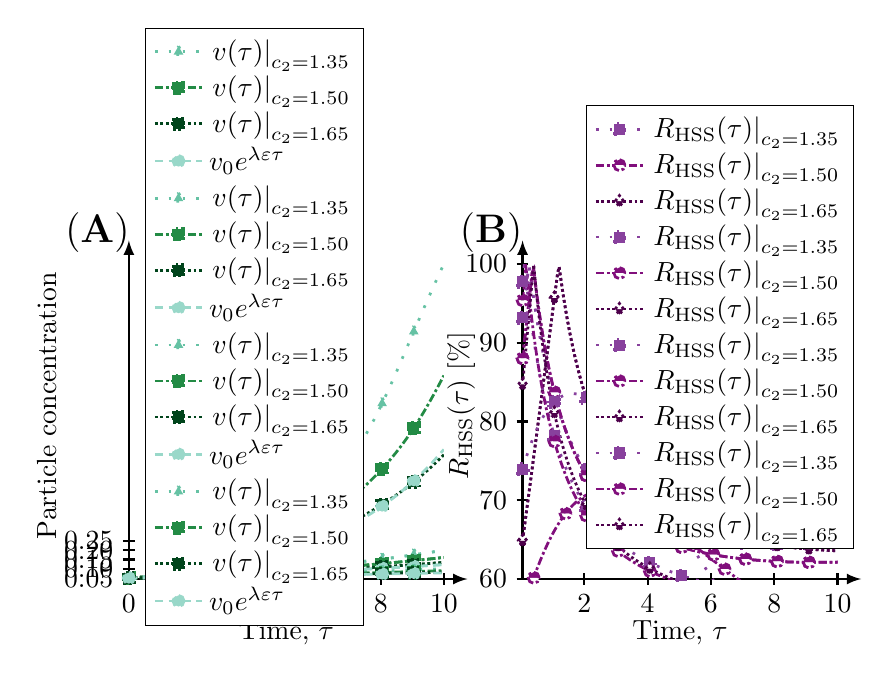
\begin{tikzpicture}
    \begin{axis}[name=plot1,height=4cm,width=4cm,xlabel={Time, $\tau$},ylabel={Particle concentration},ymin = {0.045},x label style={at={(axis description cs:0.5,-0.1)},anchor=north},y label style={at={(axis description cs:-0.2,0.55)},rotate=0,anchor=south},extra x ticks = {0}, extra y ticks= {0},legend style={at={(axis description cs:0.05,0.8)},anchor=west,nodes={scale=1.0, transform shape}},legend cell align={left},ytick={0,0.05,0.10,0.15,0.20,0.25},yticklabels={$0$,$0.05$,$0.10$,$0.15$,$0.20$,$0.25$}]
     \addplot[
color=green_3,line width=1.0pt,loosely dotted,mark=triangle*,mark repeat=20
]
coordinates {%
(0.0,0.05)
(0.05025125628140704,0.05023124434463991)
(0.10050251256281408,0.05047239161724666)
(0.15075376884422112,0.05072298656727123)
(0.20100502512562815,0.05098260690190811)
(0.2512562814070352,0.05125086034173194)
(0.30150753768844224,0.051527382465836005)
(0.35175879396984927,0.05181183499304862)
(0.4020100502512563,0.05210390405318467)
(0.45226130653266333,0.05240329705118452)
(0.5025125628140704,0.05270974155299069)
(0.5527638190954774,0.05302298576859999)
(0.6030150753768845,0.05334279497093624)
(0.6532663316582915,0.05366895075743055)
(0.7035175879396985,0.05400125038100905)
(0.7537688442211056,0.05433950537328798)
(0.8040201005025126,0.05468354062375951)
(0.8542713567839196,0.0550331934725607)
(0.9045226130653267,0.05538831291914357)
(0.9547738693467337,0.05574875883562884)
(1.0050251256281408,0.0561144012010301)
(1.0552763819095479,0.056485119498355225)
(1.105527638190955,0.05686080218190526)
(1.155778894472362,0.0572413459438094)
(1.206030150753769,0.057626655275086744)
(1.256281407035176,0.058016641951129946)
(1.306532663316583,0.05841122458349946)
(1.35678391959799,0.05881032819529648)
(1.407035175879397,0.059213883830808944)
(1.4572864321608041,0.05962182816914263)
(1.5075376884422111,0.060034103186317425)
(1.5577889447236182,0.060450655831589574)
(1.6080402010050252,0.0608714377308142)
(1.6582914572864322,0.06129640488769942)
(1.7085427135678393,0.061725517450444904)
(1.7587939698492463,0.06215873948302448)
(1.8090452261306533,0.06259603865276701)
(1.8592964824120604,0.06303738607106402)
(1.9095477386934674,0.06348275612578244)
(1.9597989949748744,0.06393212621991769)
(2.0100502512562817,0.0643854766245268)
(2.0603015075376887,0.06484279035251601)
(2.1105527638190957,0.06530405295035044)
(2.1608040201005028,0.06576925236260814)
(2.21105527638191,0.06623837883642267)
(2.261306532663317,0.0667114247524261)
(2.311557788944724,0.06718838449941462)
(2.361809045226131,0.06766925440379547)
(2.412060301507538,0.06815403259714096)
(2.462311557788945,0.06864271890542482)
(2.512562814070352,0.06913531479137497)
(2.562814070351759,0.06963182324910007)
(2.613065326633166,0.07013224870525948)
(2.663316582914573,0.07063659697578689)
(2.71356783919598,0.07114487517934893)
(2.763819095477387,0.07165709165154097)
(2.814070351758794,0.0721732559163488)
(2.864321608040201,0.07269337862246013)
(2.9145728643216082,0.07321747145097314)
(2.9648241206030153,0.07374554708628579)
(3.0150753768844223,0.07427761918159582)
(3.0653266331658293,0.07481370230029845)
(3.1155778894472363,0.07535381185474652)
(3.1658291457286434,0.07589796409534265)
(3.2160804020100504,0.0764461760675493)
(3.2663316582914574,0.07699846555599371)
(3.3165829145728645,0.07755485106333423)
(3.3668341708542715,0.07811535178851474)
(3.4170854271356785,0.07867998758889791)
(3.4673366834170856,0.07924877893687174)
(3.5175879396984926,0.0798217469168255)
(3.5678391959798996,0.08039891319618171)
(3.6180904522613067,0.08098029999263122)
(3.6683417085427137,0.08156593005854801)
(3.7185929648241207,0.08215582666659457)
(3.7688442211055277,0.08275001358646607)
(3.819095477386935,0.0833485150569165)
(3.869346733668342,0.08395135578406893)
(3.919597989949749,0.08455856092326099)
(3.969849246231156,0.08517015605657816)
(4.020100502512563,0.08578616718356306)
(4.07035175879397,0.08640662071307836)
(4.120603015075377,0.08703154344901433)
(4.170854271356784,0.08766096257074332)
(4.2211055276381915,0.08829490563267262)
(4.2713567839195985,0.0889334005538813)
(4.3216080402010055,0.0895764756054192)
(4.371859296482413,0.09022415939896555)
(4.42211055276382,0.09087648088628728)
(4.472361809045227,0.0915334693499097)
(4.522613065326634,0.09219515439147408)
(4.572864321608041,0.0928615659286396)
(4.623115577889448,0.09353273419109473)
(4.673366834170855,0.0942086897135304)
(4.723618090452262,0.09488946332621584)
(4.773869346733669,0.09557508615565179)
(4.824120603015076,0.0962655896194509)
(4.874371859296483,0.09696100542028004)
(4.92462311557789,0.09766136554133735)
(4.974874371859297,0.0983667022459807)
(5.025125628140704,0.09907704807302238)
(5.075376884422111,0.09979243583396501)
(5.125628140703518,0.10051289860683055)
(5.175879396984925,0.1012384697396514)
(5.226130653266332,0.10196918284474873)
(5.276381909547739,0.10270507179473787)
(5.326633165829146,0.10344617072521177)
(5.376884422110553,0.10419251403198446)
(5.42713567839196,0.10494413636934984)
(5.477386934673367,0.10570107264468244)
(5.527638190954774,0.10646335801957932)
(5.577889447236181,0.10723102790933192)
(5.628140703517588,0.10800411798024022)
(5.678391959798995,0.10878266415162464)
(5.728643216080402,0.10956670260041668)
(5.778894472361809,0.1103562697486513)
(5.8291457286432165,0.1111514022663016)
(5.8793969849246235,0.1119521370710238)
(5.9296482412060305,0.11275851133939964)
(5.9798994974874375,0.11357056249554492)
(6.030150753768845,0.1143883282091336)
(6.080402010050252,0.1152118463973166)
(6.130653266331659,0.11604115522775607)
(6.180904522613066,0.11687629312161649)
(6.231155778894473,0.11771729874498671)
(6.28140703517588,0.11856421101194564)
(6.331658291457287,0.1194170690851472)
(6.381909547738694,0.12027591238387501)
(6.432160804020101,0.12114078057584697)
(6.482412060301508,0.12201171357765256)
(6.532663316582915,0.12288875155620466)
(6.582914572864322,0.12377193493297692)
(6.633165829145729,0.12466130438530929)
(6.683417085427136,0.1255569008400498)
(6.733668341708543,0.1264587654770645)
(6.78391959798995,0.12736693972961075)
(6.834170854271357,0.12828146528877746)
(6.884422110552764,0.12920238410716797)
(6.934673366834171,0.1301297383901315)
(6.984924623115578,0.1310635706003772)
(7.035175879396985,0.13200392345869635)
(7.085427135678392,0.13295083994681203)
(7.135678391959799,0.1339043633113025)
(7.185929648241206,0.13486453705752935)
(7.236180904522613,0.13583140495308213)
(7.28643216080402,0.1368050110287401)
(7.336683417085427,0.1377853995808528)
(7.386934673366834,0.1387726151758404)
(7.437185929648241,0.13976670264476812)
(7.4874371859296485,0.14076770708648853)
(7.5376884422110555,0.14177567386885634)
(7.5879396984924625,0.14279064863091795)
(7.63819095477387,0.14381267728815325)
(7.688442211055277,0.1448418060271631)
(7.738693467336684,0.1458780813086689)
(7.788944723618091,0.14692154986902473)
(7.839195979899498,0.14797225874264225)
(7.889447236180905,0.14903025516965582)
(7.939698492462312,0.15009558676978152)
(7.989949748743719,0.15116830139257387)
(8.040201005025127,0.1522484471735132)
(8.090452261306533,0.15333607253550902)
(8.14070351758794,0.15443122619895483)
(8.190954773869347,0.15553395716597057)
(8.241206030150755,0.15664431472374293)
(8.291457286432161,0.15776234844632855)
(8.341708542713569,0.1588881081946541)
(8.391959798994975,0.16002164411651618)
(8.442211055276383,0.16116300669037284)
(8.492462311557789,0.16231224672047867)
(8.542713567839197,0.16346941526381853)
(8.592964824120603,0.16463456367018028)
(8.643216080402011,0.16580774358230713)
(8.693467336683417,0.16698900693589716)
(8.743718592964825,0.16817840597457634)
(8.793969849246231,0.16937599337088424)
(8.84422110552764,0.1705818220460171)
(8.894472361809045,0.17179594520127775)
(8.944723618090453,0.1730184163420357)
(8.99497487437186,0.17424928927772682)
(9.045226130653267,0.1754886181218537)
(9.095477386934673,0.1767364573788547)
(9.145728643216081,0.17799286195198794)
(9.195979899497488,0.1792578869716136)
(9.246231155778895,0.1805315878844349)
(9.296482412060302,0.18181402045432693)
(9.34673366834171,0.18310524076233692)
(9.396984924623116,0.1844053052237248)
(9.447236180904524,0.1857142707554889)
(9.49748743718593,0.18703219453905864)
(9.547738693467338,0.18835913405156765)
(9.597989949748744,0.18969514710247926)
(9.648241206030152,0.1910402918335869)
(9.698492462311558,0.19239462671901364)
(9.748743718592966,0.19375821066543625)
(9.798994974874372,0.19513110304766873)
(9.84924623115578,0.19651336347710335)
(9.899497487437186,0.1979050519139552)
(9.949748743718594,0.1993062286691996)
(10.0,0.200716954404572)
};
\addlegendentry{$\left.v(\tau)\right|_{c_{2}=1.35}$}
\addplot[
color=green_2,line width=1.0pt,densely dashdotted,mark=square*,mark repeat=20
]
coordinates {%
(0.0,0.05)
(0.05025125628140704,0.050229470275563175)
(0.10050251256281408,0.05046539268341048)
(0.15075376884422112,0.05070745072630145)
(0.20100502512562815,0.05095535186194451)
(0.2512562814070352,0.05120882539671887)
(0.30150753768844224,0.05146762088788799)
(0.35175879396984927,0.05173150663792835)
(0.4020100502512563,0.05200026872632198)
(0.45226130653266333,0.0522737087938827)
(0.5025125628140704,0.05255164296791706)
(0.5527638190954774,0.05283390201223243)
(0.6030150753768845,0.05312032906561781)
(0.6532663316582915,0.053410778994917744)
(0.7035175879396985,0.053705117755546296)
(0.7537688442211056,0.054003221469672937)
(0.8040201005025126,0.05430497570954987)
(0.8542713567839196,0.054610274818874184)
(0.9045226130653267,0.05491902131835854)
(0.9547738693467337,0.055231125321591024)
(1.0050251256281408,0.05554650394823915)
(1.0552763819095479,0.05586508090491625)
(1.105527638190955,0.05618678606803115)
(1.155778894472362,0.056511554921765995)
(1.206030150753769,0.05683932826755961)
(1.256281407035176,0.05717005181492484)
(1.306532663316583,0.05750367586712096)
(1.35678391959799,0.05784015500255203)
(1.407035175879397,0.058179447793256685)
(1.4572864321608041,0.058521516516042704)
(1.5075376884422111,0.05886632690979391)
(1.5577889447236182,0.05921384794143902)
(1.6080402010050252,0.059564051592450915)
(1.6582914572864322,0.05991691264178704)
(1.7085427135678393,0.06027240850287719)
(1.7587939698492463,0.06063051906388959)
(1.8090452261306533,0.06099122645763108)
(1.8592964824120604,0.06135451495004835)
(1.9095477386934674,0.06172037083372317)
(1.9597989949748744,0.062088782240545086)
(2.0100502512562817,0.06245973903068466)
(2.0603015075376887,0.06283323272084805)
(2.1105527638190957,0.06320925634088839)
(2.1608040201005028,0.06358780432619648)
(2.21105527638191,0.06396887247085366)
(2.261306532663317,0.0643524578150191)
(2.311557788944724,0.06473855854030386)
(2.361809045226131,0.06512717394283779)
(2.412060301507538,0.06551830434672903)
(2.462311557788945,0.06591195101832016)
(2.512562814070352,0.06630811613881982)
(2.562814070351759,0.06670680274067328)
(2.613065326633166,0.0671080146323701)
(2.663316582914573,0.06751175637749317)
(2.71356783919598,0.06791803324648969)
(2.763819095477387,0.06832685115341393)
(2.814070351758794,0.06873821663795696)
(2.864321608040201,0.06915213683127554)
(2.9145728643216082,0.06956861940363475)
(2.9648241206030153,0.06998767254014648)
(3.0150753768844223,0.07040930492240915)
(3.0653266331658293,0.0708335256914043)
(3.1155778894472363,0.07126034441511374)
(3.1658291457286434,0.07168977108071099)
(3.2160804020100504,0.07212181606709468)
(3.2663316582914574,0.07255649011271603)
(3.3165829145728645,0.07299380431049657)
(3.3668341708542715,0.07343377008873675)
(3.4170854271356785,0.07387639918462281)
(3.4673366834170856,0.07432170363538279)
(3.5175879396984926,0.07476969576703)
(3.5678391959798996,0.07522038817543827)
(3.6180904522613067,0.07567379371320829)
(3.6683417085427137,0.07612992548419355)
(3.7185929648241207,0.07658879682963607)
(3.7688442211055277,0.07705042131298058)
(3.819095477386935,0.07751481271807097)
(3.869346733668342,0.07798198503890168)
(3.919597989949749,0.07845195246684887)
(3.969849246231156,0.07892472938751684)
(4.020100502512563,0.07940033037438232)
(4.07035175879397,0.0798787701790602)
(4.120603015075377,0.08036006372630058)
(4.170854271356784,0.08084422611071553)
(4.2211055276381915,0.08133127258960925)
(4.2713567839195985,0.08182121857703925)
(4.3216080402010055,0.08231407964157225)
(4.371859296482413,0.08280987150215782)
(4.42211055276382,0.0833086100210313)
(4.472361809045227,0.0838103112048153)
(4.522613065326634,0.0843149912007395)
(4.572864321608041,0.08482266629268315)
(4.623115577889448,0.08533335289385725)
(4.673366834170855,0.08584706754869172)
(4.723618090452262,0.08636382692870485)
(4.773869346733669,0.08688364783035615)
(4.824120603015076,0.0874065471812397)
(4.874371859296483,0.08793254202737434)
(4.92462311557789,0.08846164953216862)
(4.974874371859297,0.08899388697641321)
(5.025125628140704,0.0895292717683279)
(5.075376884422111,0.09006782142880382)
(5.125628140703518,0.09060955359100578)
(5.175879396984925,0.09115448600085613)
(5.226130653266332,0.09170263652288341)
(5.276381909547739,0.09225402313145249)
(5.326633165829146,0.09280866390984067)
(5.376884422110553,0.09336657705058804)
(5.42713567839196,0.09392778086203016)
(5.477386934673367,0.09449229376025704)
(5.527638190954774,0.09506013426821053)
(5.577889447236181,0.09563132101644543)
(5.628140703517588,0.09620587274841125)
(5.678391959798995,0.09678380831395644)
(5.728643216080402,0.09736514666851946)
(5.778894472361809,0.09794990687365392)
(5.8291457286432165,0.09853810809905605)
(5.8793969849246235,0.09912976962671205)
(5.9296482412060305,0.09972491084198873)
(5.9798994974874375,0.10032355123638359)
(6.030150753768845,0.10092571040748687)
(6.080402010050252,0.10153140806252738)
(6.130653266331659,0.1021406640159948)
(6.180904522613066,0.10275349818775027)
(6.231155778894473,0.10336993060416412)
(6.28140703517588,0.10398998139869621)
(6.331658291457287,0.10461367081496065)
(6.381909547738694,0.10524101920255685)
(6.432160804020101,0.10587204701810095)
(6.482412060301508,0.10650677482554995)
(6.532663316582915,0.10714522329821921)
(6.582914572864322,0.10778741321911792)
(6.633165829145729,0.10843336547848793)
(6.683417085427136,0.109083101075214)
(6.733668341708543,0.10973664111972214)
(6.78391959798995,0.11039400682352644)
(6.834170854271357,0.11105521952044156)
(6.884422110552764,0.11172030064714238)
(6.934673366834171,0.11238927175095904)
(6.984924623115578,0.11306215449115509)
(7.035175879396985,0.11373897064011243)
(7.085427135678392,0.1144197420793925)
(7.135678391959799,0.11510449080144658)
(7.185929648241206,0.1157932389096865)
(7.236180904522613,0.11648600861848454)
(7.28643216080402,0.11718282226099998)
(7.336683417085427,0.11788370229050668)
(7.386934673366834,0.11858867126477585)
(7.437185929648241,0.11929775185389307)
(7.4874371859296485,0.12001096684033538)
(7.5376884422110555,0.12072833911897221)
(7.5879396984924625,0.12144989171268034)
(7.63819095477387,0.12217564776622757)
(7.688442211055277,0.12290563052829967)
(7.738693467336684,0.12363986336222206)
(7.788944723618091,0.12437836974595969)
(7.839195979899498,0.12512117327231945)
(7.889447236180905,0.12586829767016808)
(7.939698492462312,0.12661976678814169)
(7.989949748743719,0.12737560458210703)
(8.040201005025127,0.12813583512514642)
(8.090452261306533,0.12890048260755774)
(8.14070351758794,0.12966957133770138)
(8.190954773869347,0.13044312576796388)
(8.241206030150755,0.13122117046805443)
(8.291457286432161,0.1320037301189868)
(8.341708542713569,0.13279082952186014)
(8.391959798994975,0.1335824935978587)
(8.442211055276383,0.13437874739018554)
(8.492462311557789,0.1351796160915588)
(8.542713567839197,0.13598512501002458)
(8.592964824120603,0.13679529956981565)
(8.643216080402011,0.13761016531819087)
(8.693467336683417,0.138429747925435)
(8.743718592964825,0.13925407318854044)
(8.793969849246231,0.14008316705982085)
(8.84422110552764,0.14091705560534457)
(8.894472361809045,0.14175576501207082)
(8.944723618090453,0.1425993215931239)
(8.99497487437186,0.14344775178779282)
(9.045226130653267,0.14430108216777635)
(9.095477386934673,0.14515933946526946)
(9.145728643216081,0.14602255052528956)
(9.195979899497488,0.14689074231858126)
(9.246231155778895,0.14776394194543147)
(9.296482412060302,0.14864217663566917)
(9.34673366834171,0.1495254737582906)
(9.396984924623116,0.15041386084619163)
(9.447236180904524,0.15130736554541663)
(9.49748743718593,0.15220601563269456)
(9.547738693467338,0.15310983901787015)
(9.597989949748744,0.15401886374390353)
(9.648241206030152,0.15493311800108772)
(9.698492462311558,0.15585263014581097)
(9.748743718592966,0.1567774286490339)
(9.798994974874372,0.1577075421173634)
(9.84924623115578,0.15864299929434983)
(9.899497487437186,0.15958382906048688)
(9.949748743718594,0.1605300604535704)
(10.0,0.16148172267791244)
};
\addlegendentry{$\left.v(\tau)\right|_{c_{2}=1.50}$}
\addplot[
color=green_1,line width=1.0pt, densely dotted, mark=square*,mark repeat=20
]
coordinates {%
(0.0,0.05)
(0.05025125628140704,0.05022770510607874)
(0.10050251256281408,0.05045846285524487)
(0.15075376884422112,0.05069214284528406)
(0.20100502512562815,0.05092862500998075)
(0.2512562814070352,0.05116779916332797)
(0.30150753768844224,0.05140956400954679)
(0.35175879396984927,0.05165382650457791)
(0.4020100502512563,0.05190050116474278)
(0.45226130653266333,0.05214950975012218)
(0.5025125628140704,0.05240078063473372)
(0.5527638190954774,0.05265424783783952)
(0.6030150753768845,0.052909850600238804)
(0.6532663316582915,0.05316753394344876)
(0.7035175879396985,0.05342724757157773)
(0.7537688442211056,0.053688945205000484)
(0.8040201005025126,0.05395258473113585)
(0.8542713567839196,0.05421812777204374)
(0.9045226130653267,0.05448553939532375)
(0.9547738693467337,0.05475478783956584)
(1.0050251256281408,0.05502584426452787)
(1.0552763819095479,0.055298682568133216)
(1.105527638190955,0.05557327916184044)
(1.155778894472362,0.055849612777758774)
(1.206030150753769,0.05612766427492754)
(1.256281407035176,0.056407416548052265)
(1.306532663316583,0.05668885429030559)
(1.35678391959799,0.056971963939877246)
(1.407035175879397,0.057256733475184715)
(1.4572864321608041,0.05754315236775956)
(1.5075376884422111,0.05783121141286077)
(1.5577889447236182,0.05812090268257436)
(1.6080402010050252,0.05841221939274175)
(1.6582914572864322,0.058705155845200106)
(1.7085427135678393,0.05899970733318024)
(1.7587939698492463,0.059295870076844)
(1.8090452261306533,0.05959364115454163)
(1.8592964824120604,0.05989301842102896)
(1.9095477386934674,0.06019400047938445)
(1.9597989949748744,0.06049658663520471)
(2.0100502512562817,0.06080077684265179)
(2.0603015075376887,0.06110657159517956)
(2.1105527638190957,0.06141397196124116)
(2.1608040201005028,0.06172297951664779)
(2.21105527638191,0.062033596300833126)
(2.261306532663317,0.062345824802948466)
(2.311557788944724,0.062659667920316)
(2.361809045226131,0.06297512893586907)
(2.412060301507538,0.06329221149442475)
(2.462311557788945,0.06361091956109274)
(2.512562814070352,0.06393125741176789)
(2.562814070351759,0.06425322961146893)
(2.613065326633166,0.06457684099731877)
(2.663316582914573,0.06490209665977799)
(2.71356783919598,0.06522900192265124)
(2.763819095477387,0.06555756233128453)
(2.814070351758794,0.06588778364472293)
(2.864321608040201,0.06621967181245562)
(2.9145728643216082,0.06655323296200776)
(2.9648241206030153,0.06688847339149817)
(3.0150753768844223,0.06722539956522963)
(3.0653266331658293,0.06756401810253712)
(3.1155778894472363,0.06790433575762005)
(3.1658291457286434,0.068246359425668)
(3.2160804020100504,0.06859009613621184)
(3.2663316582914574,0.06893555303158792)
(3.3165829145728645,0.06928273737224964)
(3.3668341708542715,0.06963165653270244)
(3.4170854271356785,0.06998231798421)
(3.4673366834170856,0.07033472929946853)
(3.5175879396984926,0.07068889815145955)
(3.5678391959798996,0.07104483229739925)
(3.6180904522613067,0.07140253958442663)
(3.6683417085427137,0.07176202794800667)
(3.7185929648241207,0.07212330539494784)
(3.7688442211055277,0.0724863800036894)
(3.819095477386935,0.07285125992885952)
(3.869346733668342,0.07321795341646195)
(3.919597989949749,0.07358646876871139)
(3.969849246231156,0.07395681435118663)
(4.020100502512563,0.07432899859336947)
(4.07035175879397,0.07470303000142828)
(4.120603015075377,0.07507891713657842)
(4.170854271356784,0.07545666861654833)
(4.2211055276381915,0.07583629311551215)
(4.2713567839195985,0.07621779937348168)
(4.3216080402010055,0.07660119618394803)
(4.371859296482413,0.07698649239162807)
(4.42211055276382,0.07737369689287514)
(4.472361809045227,0.07776281864440479)
(4.522613065326634,0.07815386665662476)
(4.572864321608041,0.07854684998770889)
(4.623115577889448,0.07894177774565403)
(4.673366834170855,0.0793386590885823)
(4.723618090452262,0.07973750323567066)
(4.773869346733669,0.08013831944021825)
(4.824120603015076,0.08054111701058798)
(4.874371859296483,0.08094590530346703)
(4.92462311557789,0.08135269372644421)
(4.974874371859297,0.08176149173129338)
(5.025125628140704,0.0821723088166246)
(5.075376884422111,0.08258515452805842)
(5.125628140703518,0.08300003846075647)
(5.175879396984925,0.08341697025741888)
(5.226130653266332,0.08383595960727319)
(5.276381909547739,0.08425701624694655)
(5.326633165829146,0.08468014995930664)
(5.376884422110553,0.08510537056862245)
(5.42713567839196,0.08553268794815855)
(5.477386934673367,0.08596211201821617)
(5.527638190954774,0.08639365274560976)
(5.577889447236181,0.08682732014197321)
(5.628140703517588,0.087263124263719)
(5.678391959798995,0.08770107521461928)
(5.728643216080402,0.08814118314453691)
(5.778894472361809,0.08858345761397649)
(5.8291457286432165,0.08902791055434814)
(5.8793969849246235,0.08947455095195865)
(5.9296482412060305,0.08992338926953639)
(5.9798994974874375,0.09037443596980974)
(6.030150753768845,0.09082770155303856)
(6.080402010050252,0.09128319660000735)
(6.130653266331659,0.09174093162228196)
(6.180904522613066,0.09220091712720252)
(6.231155778894473,0.09266316362210919)
(6.28140703517588,0.09312768161510385)
(6.331658291457287,0.09359448200114646)
(6.381909547738694,0.09406357576302606)
(6.432160804020101,0.09453497362995142)
(6.482412060301508,0.09500868633113137)
(6.532663316582915,0.09548472459577469)
(6.582914572864322,0.09596309920502906)
(6.633165829145729,0.09644382155651167)
(6.683417085427136,0.09692690279519559)
(6.733668341708543,0.09741235392049959)
(6.78391959798995,0.09790018593184241)
(6.834170854271357,0.09839040982864279)
(6.884422110552764,0.09888303679963331)
(6.934673366834171,0.09937807857736751)
(6.984924623115578,0.09987554647564419)
(7.035175879396985,0.10037545176777907)
(7.085427135678392,0.10087780572708789)
(7.135678391959799,0.10138261962688641)
(7.185929648241206,0.1018899052072866)
(7.236180904522613,0.10239967442185269)
(7.28643216080402,0.10291193881849134)
(7.336683417085427,0.10342670994497277)
(7.386934673366834,0.10394399934906716)
(7.437185929648241,0.10446381857854474)
(7.4874371859296485,0.10498617937094763)
(7.5376884422110555,0.10551109422701162)
(7.5879396984924625,0.10603857510323417)
(7.63819095477387,0.1065686338716313)
(7.688442211055277,0.10710128240421905)
(7.738693467336684,0.10763653257301346)
(7.788944723618091,0.10817439626973781)
(7.839195979899498,0.10871488614221383)
(7.889447236180905,0.10925801470128603)
(7.939698492462312,0.10980379414571291)
(7.989949748743719,0.11035223667425295)
(8.040201005025127,0.11090335448566468)
(8.090452261306533,0.11145715977870659)
(8.14070351758794,0.1120136672554292)
(8.190954773869347,0.11257288462399978)
(8.241206030150755,0.11313482829419372)
(8.291457286432161,0.11369951058470296)
(8.341708542713569,0.11426694386642591)
(8.391959798994975,0.11483714056246733)
(8.442211055276383,0.11541011322871936)
(8.492462311557789,0.11598587520937231)
(8.542713567839197,0.1165644394985542)
(8.592964824120603,0.11714581899735876)
(8.643216080402011,0.11773002667790905)
(8.693467336683417,0.11831707558335729)
(8.743718592964825,0.11890697882788505)
(8.793969849246231,0.11949974959670308)
(8.84422110552764,0.12009540114605145)
(8.894472361809045,0.12069394680319942)
(8.944723618090453,0.12129539996644557)
(8.99497487437186,0.12189977410511765)
(9.045226130653267,0.12250708275956879)
(9.095477386934673,0.12311733934611879)
(9.145728643216081,0.12373055729439207)
(9.195979899497488,0.12434675026096725)
(9.246231155778895,0.12496593196648467)
(9.296482412060302,0.12558811619564614)
(9.34673366834171,0.12621331679721523)
(9.396984924623116,0.126841547684017)
(9.447236180904524,0.12747282283293818)
(9.49748743718593,0.12810715628492708)
(9.547738693467338,0.12874456214499366)
(9.597989949748744,0.1293850545822094)
(9.648241206030152,0.13002864782970747)
(9.698492462311558,0.1306753561215794)
(9.748743718592966,0.13132519353078007)
(9.798994974874372,0.13197817437228415)
(9.84924623115578,0.13263431304313367)
(9.899497487437186,0.13329362399806616)
(9.949748743718594,0.1339561217495148)
(10.0,0.13462182086760824)
};
\addlegendentry{$\left.v(\tau)\right|_{c_{2}=1.65}$}
\addplot[
color=green_4,line width=1.0pt,densely dashed, mark=otimes*,mark repeat=20
]
coordinates {%
(0.0,0.05)
(0.05025125628140704,0.05022664435321215)
(0.10050251256281408,0.05045431605968114)
(0.15075376884422112,0.05068301977628329)
(0.20100502512562815,0.05091276018100397)
(0.2512562814070352,0.051143541973033335)
(0.30150753768844224,0.05137536987286247)
(0.35175879396984927,0.05160824862237985)
(0.4020100502512563,0.05184218298496847)
(0.45226130653266333,0.052077177745603144)
(0.5025125628140704,0.05231323771094846)
(0.5527638190954774,0.052550367709457084)
(0.6030150753768845,0.05278857259146848)
(0.6532663316582915,0.053027857229308195)
(0.7035175879396985,0.05326822651738744)
(0.7537688442211056,0.053509685372303266)
(0.8040201005025126,0.05375223873293908)
(0.8542713567839196,0.053995891560565716)
(0.9045226130653267,0.054240648838942855)
(0.9547738693467337,0.05448651557442104)
(1.0050251256281408,0.054733496796044)
(1.0552763819095479,0.05498159755565157)
(1.105527638190955,0.05523082292798298)
(1.155778894472362,0.05548117801078072)
(1.206030150753769,0.055732667924894744)
(1.256281407035176,0.05598529781438724)
(1.306532663316583,0.056239072846637865)
(1.35678391959799,0.056493998212449395)
(1.407035175879397,0.056750079126153964)
(1.4572864321608041,0.057007320825719666)
(1.5075376884422111,0.057265728572857715)
(1.5577889447236182,0.057525307653130055)
(1.6080402010050252,0.05778606337605752)
(1.6582914572864322,0.05804800107522837)
(1.7085427135678393,0.05831112610840742)
(1.7587939698492463,0.05857544385764566)
(1.8090452261306533,0.05884095972939027)
(1.8592964824120604,0.05910767915459525)
(1.9095477386934674,0.05937560758883253)
(1.9597989949748744,0.059644750512403505)
(2.0100502512562817,0.059915113430451174)
(2.0603015075376887,0.06018670187307271)
(2.1105527638190957,0.06045952139543259)
(2.1608040201005028,0.060733577577876265)
(2.21105527638191,0.06100887602604421)
(2.261306532663317,0.06128542237098666)
(2.311557788944724,0.06156322226927877)
(2.361809045226131,0.06184228140313628)
(2.412060301507538,0.06212260548053183)
(2.462311557788945,0.0624042002353116)
(2.512562814070352,0.06268707142731265)
(2.562814070351759,0.06297122484248079)
(2.613065326633166,0.0632566662929888)
(2.663316582914573,0.0635434016173554)
(2.71356783919598,0.06383143668056471)
(2.763819095477387,0.06412077737418607)
(2.814070351758794,0.06441142961649471)
(2.864321608040201,0.06470339935259271)
(2.9145728643216082,0.06499669255453061)
(2.9648241206030153,0.06529131522142961)
(3.0150753768844223,0.06558727337960422)
(3.0653266331658293,0.06588457308268561)
(3.1155778894472363,0.06618322041174528)
(3.1658291457286434,0.0664832214754196)
(3.2160804020100504,0.06678458241003472)
(3.2663316582914574,0.06708730937973204)
(3.3165829145728645,0.06739140857659427)
(3.3668341708542715,0.06769688622077222)
(3.4170854271356785,0.06800374856061188)
(3.4673366834170856,0.06831200187278229)
(3.5175879396984926,0.06862165246240397)
(3.5678391959798996,0.06893270666317776)
(3.6180904522613067,0.06924517083751452)
(3.6683417085427137,0.06955905137666518)
(3.7185929648241207,0.06987435470085147)
(3.7688442211055277,0.07019108725939728)
(3.819095477386935,0.07050925553086053)
(3.869346733668342,0.07082886602316577)
(3.919597989949749,0.07114992527373716)
(3.969849246231156,0.07147243984963234)
(4.020100502512563,0.07179641634767661)
(4.07035175879397,0.07212186139459797)
(4.120603015075377,0.07244878164716266)
(4.170854271356784,0.07277718379231124)
(4.2211055276381915,0.07310707454729544)
(4.2713567839195985,0.0734384606598155)
(4.3216080402010055,0.07377134890815829)
(4.371859296482413,0.07410574610133583)
(4.42211055276382,0.07444165907922463)
(4.472361809045227,0.07477909471270563)
(4.522613065326634,0.07511805990380464)
(4.572864321608041,0.07545856158583361)
(4.623115577889448,0.07580060672353241)
(4.673366834170855,0.07614420231321128)
(4.723618090452262,0.07648935538289392)
(4.773869346733669,0.07683607299246131)
(4.824120603015076,0.07718436223379606)
(4.874371859296483,0.07753423023092747)
(4.92462311557789,0.07788568414017727)
(4.974874371859297,0.07823873115030597)
(5.025125628140704,0.07859337848265996)
(5.075376884422111,0.07894963339131916)
(5.125628140703518,0.07930750316324538)
(5.175879396984925,0.07966699511843145)
(5.226130653266332,0.08002811661005088)
(5.276381909547739,0.0803908750246083)
(5.326633165829146,0.08075527778209052)
(5.376884422110553,0.08112133233611829)
(5.42713567839196,0.08148904617409881)
(5.477386934673367,0.08185842681737888)
(5.527638190954774,0.08222948182139865)
(5.577889447236181,0.08260221877584625)
(5.628140703517588,0.08297664530481304)
(5.678391959798995,0.0833527690669495)
(5.728643216080402,0.08373059775562189)
(5.778894472361809,0.08411013909906967)
(5.8291457286432165,0.0844914008605635)
(5.8793969849246235,0.08487439083856411)
(5.9296482412060305,0.08525911686688174)
(5.9798994974874375,0.08564558681483639)
(6.030150753768845,0.08603380858741884)
(6.080402010050252,0.08642379012545232)
(6.130653266331659,0.0868155394057548)
(6.180904522613066,0.08720906444130241)
(6.231155778894473,0.08760437328139312)
(6.28140703517588,0.08800147401181144)
(6.331658291457287,0.08840037475499388)
(6.381909547738694,0.08880108367019501)
(6.432160804020101,0.08920360895365438)
(6.482412060301508,0.08960795883876417)
(6.532663316582915,0.09001414159623762)
(6.582914572864322,0.09042216553427812)
(6.633165829145729,0.09083203899874927)
(6.683417085427136,0.09124377037334552)
(6.733668341708543,0.09165736807976359)
(6.78391959798995,0.09207284057787489)
(6.834170854271357,0.09249019636589845)
(6.884422110552764,0.0929094439805747)
(6.934673366834171,0.09333059199734023)
(6.984924623115578,0.09375364903050311)
(7.035175879396985,0.09417862373341904)
(7.085427135678392,0.09460552479866845)
(7.135678391959799,0.09503436095823424)
(7.185929648241206,0.09546514098368039)
(7.236180904522613,0.09589787368633143)
(7.28643216080402,0.09633256791745261)
(7.336683417085427,0.09676923256843091)
(7.386934673366834,0.09720787657095707)
(7.437185929648241,0.09764850889720807)
(7.4874371859296485,0.09809113856003082)
(7.5376884422110555,0.09853577461312645)
(7.5879396984924625,0.09898242615123543)
(7.63819095477387,0.09943110231032373)
(7.688442211055277,0.09988181226776961)
(7.738693467336684,0.10033456524255131)
(7.788944723618091,0.10078937049543571)
(7.839195979899498,0.10124623732916765)
(7.889447236180905,0.10170517508866028)
(7.939698492462312,0.10216619316118623)
(7.989949748743719,0.10262930097656951)
(8.040201005025127,0.10309450800737847)
(8.090452261306533,0.1035618237691196)
(8.14070351758794,0.10403125782043204)
(8.190954773869347,0.10450281976328318)
(8.241206030150755,0.10497651924316508)
(8.291457286432161,0.10545236594929167)
(8.341708542713569,0.10593036961479702)
(8.391959798994975,0.10641054001693438)
(8.442211055276383,0.10689288697727624)
(8.492462311557789,0.1073774203619151)
(8.542713567839197,0.10786415008166539)
(8.592964824120603,0.10835308609226611)
(8.643216080402011,0.10884423839458456)
(8.693467336683417,0.10933761703482073)
(8.743718592964825,0.10983323210471302)
(8.793969849246231,0.11033109374174442)
(8.84422110552764,0.11083121212935015)
(8.894472361809045,0.11133359749712562)
(8.944723618090453,0.11183826012103598)
(8.99497487437186,0.11234521032362604)
(9.045226130653267,0.11285445847423166)
(9.095477386934673,0.11336601498919162)
(9.145728643216081,0.11387989033206088)
(9.195979899497488,0.11439609501382447)
(9.246231155778895,0.11491463959311253)
(9.296482412060302,0.11543553467641628)
(9.34673366834171,0.11595879091830497)
(9.396984924623116,0.11648441902164378)
(9.447236180904524,0.11701242973781284)
(9.49748743718593,0.11754283386692699)
(9.547738693467338,0.11807564225805683)
(9.597989949748744,0.11861086580945053)
(9.648241206030152,0.11914851546875685)
(9.698492462311558,0.1196886022332489)
(9.748743718592966,0.1202311371500493)
(9.798994974874372,0.12077613131635596)
(9.84924623115578,0.12132359587966918)
(9.899497487437186,0.12187354203801955)
(9.949748743718594,0.12242598104019715)
(10.0,0.12298092418598149)
};
\addlegendentry{$v_{0}e^{\lambda\varepsilon\tau}$}
\addplot[
color=green_3,line width=1.0pt,loosely dotted,mark=triangle*,mark repeat=20
]
coordinates {%
(0.0,0.05)
(0.05025125628140704,0.05023124434463991)
(0.10050251256281408,0.05047239161724666)
(0.15075376884422112,0.05072298656727123)
(0.20100502512562815,0.05098260690190811)
(0.2512562814070352,0.05125086034173194)
(0.30150753768844224,0.051527382465836005)
(0.35175879396984927,0.05181183499304862)
(0.4020100502512563,0.05210390405318467)
(0.45226130653266333,0.05240329705118452)
(0.5025125628140704,0.05270974155299069)
(0.5527638190954774,0.05302298576859999)
(0.6030150753768845,0.05334279497093624)
(0.6532663316582915,0.05366895075743055)
(0.7035175879396985,0.05400125038100905)
(0.7537688442211056,0.05433950537328798)
(0.8040201005025126,0.05468354062375951)
(0.8542713567839196,0.0550331934725607)
(0.9045226130653267,0.05538831291914357)
(0.9547738693467337,0.05574875883562884)
(1.0050251256281408,0.0561144012010301)
(1.0552763819095479,0.056485119498355225)
(1.105527638190955,0.05686080218190526)
(1.155778894472362,0.0572413459438094)
(1.206030150753769,0.057626655275086744)
(1.256281407035176,0.058016641951129946)
(1.306532663316583,0.05841122458349946)
(1.35678391959799,0.05881032819529648)
(1.407035175879397,0.059213883830808944)
(1.4572864321608041,0.05962182816914263)
(1.5075376884422111,0.060034103186317425)
(1.5577889447236182,0.060450655831589574)
(1.6080402010050252,0.0608714377308142)
(1.6582914572864322,0.06129640488769942)
(1.7085427135678393,0.061725517450444904)
(1.7587939698492463,0.06215873948302448)
(1.8090452261306533,0.06259603865276701)
(1.8592964824120604,0.06303738607106402)
(1.9095477386934674,0.06348275612578244)
(1.9597989949748744,0.06393212621991769)
(2.0100502512562817,0.0643854766245268)
(2.0603015075376887,0.06484279035251601)
(2.1105527638190957,0.06530405295035044)
(2.1608040201005028,0.06576925236260814)
(2.21105527638191,0.06623837883642267)
(2.261306532663317,0.0667114247524261)
(2.311557788944724,0.06718838449941462)
(2.361809045226131,0.06766925440379547)
(2.412060301507538,0.06815403259714096)
(2.462311557788945,0.06864271890542482)
(2.512562814070352,0.06913531479137497)
(2.562814070351759,0.06963182324910007)
(2.613065326633166,0.07013224870525948)
(2.663316582914573,0.07063659697578689)
(2.71356783919598,0.07114487517934893)
(2.763819095477387,0.07165709165154097)
(2.814070351758794,0.0721732559163488)
(2.864321608040201,0.07269337862246013)
(2.9145728643216082,0.07321747145097314)
(2.9648241206030153,0.07374554708628579)
(3.0150753768844223,0.07427761918159582)
(3.0653266331658293,0.07481370230029845)
(3.1155778894472363,0.07535381185474652)
(3.1658291457286434,0.07589796409534265)
(3.2160804020100504,0.0764461760675493)
(3.2663316582914574,0.07699846555599371)
(3.3165829145728645,0.07755485106333423)
(3.3668341708542715,0.07811535178851474)
(3.4170854271356785,0.07867998758889791)
(3.4673366834170856,0.07924877893687174)
(3.5175879396984926,0.0798217469168255)
(3.5678391959798996,0.08039891319618171)
(3.6180904522613067,0.08098029999263122)
(3.6683417085427137,0.08156593005854801)
(3.7185929648241207,0.08215582666659457)
(3.7688442211055277,0.08275001358646607)
(3.819095477386935,0.0833485150569165)
(3.869346733668342,0.08395135578406893)
(3.919597989949749,0.08455856092326099)
(3.969849246231156,0.08517015605657816)
(4.020100502512563,0.08578616718356306)
(4.07035175879397,0.08640662071307836)
(4.120603015075377,0.08703154344901433)
(4.170854271356784,0.08766096257074332)
(4.2211055276381915,0.08829490563267262)
(4.2713567839195985,0.0889334005538813)
(4.3216080402010055,0.0895764756054192)
(4.371859296482413,0.09022415939896555)
(4.42211055276382,0.09087648088628728)
(4.472361809045227,0.0915334693499097)
(4.522613065326634,0.09219515439147408)
(4.572864321608041,0.0928615659286396)
(4.623115577889448,0.09353273419109473)
(4.673366834170855,0.0942086897135304)
(4.723618090452262,0.09488946332621584)
(4.773869346733669,0.09557508615565179)
(4.824120603015076,0.0962655896194509)
(4.874371859296483,0.09696100542028004)
(4.92462311557789,0.09766136554133735)
(4.974874371859297,0.0983667022459807)
(5.025125628140704,0.09907704807302238)
(5.075376884422111,0.09979243583396501)
(5.125628140703518,0.10051289860683055)
(5.175879396984925,0.1012384697396514)
(5.226130653266332,0.10196918284474873)
(5.276381909547739,0.10270507179473787)
(5.326633165829146,0.10344617072521177)
(5.376884422110553,0.10419251403198446)
(5.42713567839196,0.10494413636934984)
(5.477386934673367,0.10570107264468244)
(5.527638190954774,0.10646335801957932)
(5.577889447236181,0.10723102790933192)
(5.628140703517588,0.10800411798024022)
(5.678391959798995,0.10878266415162464)
(5.728643216080402,0.10956670260041668)
(5.778894472361809,0.1103562697486513)
(5.8291457286432165,0.1111514022663016)
(5.8793969849246235,0.1119521370710238)
(5.9296482412060305,0.11275851133939964)
(5.9798994974874375,0.11357056249554492)
(6.030150753768845,0.1143883282091336)
(6.080402010050252,0.1152118463973166)
(6.130653266331659,0.11604115522775607)
(6.180904522613066,0.11687629312161649)
(6.231155778894473,0.11771729874498671)
(6.28140703517588,0.11856421101194564)
(6.331658291457287,0.1194170690851472)
(6.381909547738694,0.12027591238387501)
(6.432160804020101,0.12114078057584697)
(6.482412060301508,0.12201171357765256)
(6.532663316582915,0.12288875155620466)
(6.582914572864322,0.12377193493297692)
(6.633165829145729,0.12466130438530929)
(6.683417085427136,0.1255569008400498)
(6.733668341708543,0.1264587654770645)
(6.78391959798995,0.12736693972961075)
(6.834170854271357,0.12828146528877746)
(6.884422110552764,0.12920238410716797)
(6.934673366834171,0.1301297383901315)
(6.984924623115578,0.1310635706003772)
(7.035175879396985,0.13200392345869635)
(7.085427135678392,0.13295083994681203)
(7.135678391959799,0.1339043633113025)
(7.185929648241206,0.13486453705752935)
(7.236180904522613,0.13583140495308213)
(7.28643216080402,0.1368050110287401)
(7.336683417085427,0.1377853995808528)
(7.386934673366834,0.1387726151758404)
(7.437185929648241,0.13976670264476812)
(7.4874371859296485,0.14076770708648853)
(7.5376884422110555,0.14177567386885634)
(7.5879396984924625,0.14279064863091795)
(7.63819095477387,0.14381267728815325)
(7.688442211055277,0.1448418060271631)
(7.738693467336684,0.1458780813086689)
(7.788944723618091,0.14692154986902473)
(7.839195979899498,0.14797225874264225)
(7.889447236180905,0.14903025516965582)
(7.939698492462312,0.15009558676978152)
(7.989949748743719,0.15116830139257387)
(8.040201005025127,0.1522484471735132)
(8.090452261306533,0.15333607253550902)
(8.14070351758794,0.15443122619895483)
(8.190954773869347,0.15553395716597057)
(8.241206030150755,0.15664431472374293)
(8.291457286432161,0.15776234844632855)
(8.341708542713569,0.1588881081946541)
(8.391959798994975,0.16002164411651618)
(8.442211055276383,0.16116300669037284)
(8.492462311557789,0.16231224672047867)
(8.542713567839197,0.16346941526381853)
(8.592964824120603,0.16463456367018028)
(8.643216080402011,0.16580774358230713)
(8.693467336683417,0.16698900693589716)
(8.743718592964825,0.16817840597457634)
(8.793969849246231,0.16937599337088424)
(8.84422110552764,0.1705818220460171)
(8.894472361809045,0.17179594520127775)
(8.944723618090453,0.1730184163420357)
(8.99497487437186,0.17424928927772682)
(9.045226130653267,0.1754886181218537)
(9.095477386934673,0.1767364573788547)
(9.145728643216081,0.17799286195198794)
(9.195979899497488,0.1792578869716136)
(9.246231155778895,0.1805315878844349)
(9.296482412060302,0.18181402045432693)
(9.34673366834171,0.18310524076233692)
(9.396984924623116,0.1844053052237248)
(9.447236180904524,0.1857142707554889)
(9.49748743718593,0.18703219453905864)
(9.547738693467338,0.18835913405156765)
(9.597989949748744,0.18969514710247926)
(9.648241206030152,0.1910402918335869)
(9.698492462311558,0.19239462671901364)
(9.748743718592966,0.19375821066543625)
(9.798994974874372,0.19513110304766873)
(9.84924623115578,0.19651336347710335)
(9.899497487437186,0.1979050519139552)
(9.949748743718594,0.1993062286691996)
(10.0,0.200716954404572)
};
\addlegendentry{$\left.v(\tau)\right|_{c_{2}=1.35}$}
\addplot[
color=green_2,line width=1.0pt,densely dashdotted,mark=square*,mark repeat=20
]
coordinates {%
(0.0,0.05)
(0.05025125628140704,0.050229470275563175)
(0.10050251256281408,0.05046539268341048)
(0.15075376884422112,0.05070745072630145)
(0.20100502512562815,0.05095535186194451)
(0.2512562814070352,0.05120882539671887)
(0.30150753768844224,0.05146762088788799)
(0.35175879396984927,0.05173150663792835)
(0.4020100502512563,0.05200026872632198)
(0.45226130653266333,0.0522737087938827)
(0.5025125628140704,0.05255164296791706)
(0.5527638190954774,0.05283390201223243)
(0.6030150753768845,0.05312032906561781)
(0.6532663316582915,0.053410778994917744)
(0.7035175879396985,0.053705117755546296)
(0.7537688442211056,0.054003221469672937)
(0.8040201005025126,0.05430497570954987)
(0.8542713567839196,0.054610274818874184)
(0.9045226130653267,0.05491902131835854)
(0.9547738693467337,0.055231125321591024)
(1.0050251256281408,0.05554650394823915)
(1.0552763819095479,0.05586508090491625)
(1.105527638190955,0.05618678606803115)
(1.155778894472362,0.056511554921765995)
(1.206030150753769,0.05683932826755961)
(1.256281407035176,0.05717005181492484)
(1.306532663316583,0.05750367586712096)
(1.35678391959799,0.05784015500255203)
(1.407035175879397,0.058179447793256685)
(1.4572864321608041,0.058521516516042704)
(1.5075376884422111,0.05886632690979391)
(1.5577889447236182,0.05921384794143902)
(1.6080402010050252,0.059564051592450915)
(1.6582914572864322,0.05991691264178704)
(1.7085427135678393,0.06027240850287719)
(1.7587939698492463,0.06063051906388959)
(1.8090452261306533,0.06099122645763108)
(1.8592964824120604,0.06135451495004835)
(1.9095477386934674,0.06172037083372317)
(1.9597989949748744,0.062088782240545086)
(2.0100502512562817,0.06245973903068466)
(2.0603015075376887,0.06283323272084805)
(2.1105527638190957,0.06320925634088839)
(2.1608040201005028,0.06358780432619648)
(2.21105527638191,0.06396887247085366)
(2.261306532663317,0.0643524578150191)
(2.311557788944724,0.06473855854030386)
(2.361809045226131,0.06512717394283779)
(2.412060301507538,0.06551830434672903)
(2.462311557788945,0.06591195101832016)
(2.512562814070352,0.06630811613881982)
(2.562814070351759,0.06670680274067328)
(2.613065326633166,0.0671080146323701)
(2.663316582914573,0.06751175637749317)
(2.71356783919598,0.06791803324648969)
(2.763819095477387,0.06832685115341393)
(2.814070351758794,0.06873821663795696)
(2.864321608040201,0.06915213683127554)
(2.9145728643216082,0.06956861940363475)
(2.9648241206030153,0.06998767254014648)
(3.0150753768844223,0.07040930492240915)
(3.0653266331658293,0.0708335256914043)
(3.1155778894472363,0.07126034441511374)
(3.1658291457286434,0.07168977108071099)
(3.2160804020100504,0.07212181606709468)
(3.2663316582914574,0.07255649011271603)
(3.3165829145728645,0.07299380431049657)
(3.3668341708542715,0.07343377008873675)
(3.4170854271356785,0.07387639918462281)
(3.4673366834170856,0.07432170363538279)
(3.5175879396984926,0.07476969576703)
(3.5678391959798996,0.07522038817543827)
(3.6180904522613067,0.07567379371320829)
(3.6683417085427137,0.07612992548419355)
(3.7185929648241207,0.07658879682963607)
(3.7688442211055277,0.07705042131298058)
(3.819095477386935,0.07751481271807097)
(3.869346733668342,0.07798198503890168)
(3.919597989949749,0.07845195246684887)
(3.969849246231156,0.07892472938751684)
(4.020100502512563,0.07940033037438232)
(4.07035175879397,0.0798787701790602)
(4.120603015075377,0.08036006372630058)
(4.170854271356784,0.08084422611071553)
(4.2211055276381915,0.08133127258960925)
(4.2713567839195985,0.08182121857703925)
(4.3216080402010055,0.08231407964157225)
(4.371859296482413,0.08280987150215782)
(4.42211055276382,0.0833086100210313)
(4.472361809045227,0.0838103112048153)
(4.522613065326634,0.0843149912007395)
(4.572864321608041,0.08482266629268315)
(4.623115577889448,0.08533335289385725)
(4.673366834170855,0.08584706754869172)
(4.723618090452262,0.08636382692870485)
(4.773869346733669,0.08688364783035615)
(4.824120603015076,0.0874065471812397)
(4.874371859296483,0.08793254202737434)
(4.92462311557789,0.08846164953216862)
(4.974874371859297,0.08899388697641321)
(5.025125628140704,0.0895292717683279)
(5.075376884422111,0.09006782142880382)
(5.125628140703518,0.09060955359100578)
(5.175879396984925,0.09115448600085613)
(5.226130653266332,0.09170263652288341)
(5.276381909547739,0.09225402313145249)
(5.326633165829146,0.09280866390984067)
(5.376884422110553,0.09336657705058804)
(5.42713567839196,0.09392778086203016)
(5.477386934673367,0.09449229376025704)
(5.527638190954774,0.09506013426821053)
(5.577889447236181,0.09563132101644543)
(5.628140703517588,0.09620587274841125)
(5.678391959798995,0.09678380831395644)
(5.728643216080402,0.09736514666851946)
(5.778894472361809,0.09794990687365392)
(5.8291457286432165,0.09853810809905605)
(5.8793969849246235,0.09912976962671205)
(5.9296482412060305,0.09972491084198873)
(5.9798994974874375,0.10032355123638359)
(6.030150753768845,0.10092571040748687)
(6.080402010050252,0.10153140806252738)
(6.130653266331659,0.1021406640159948)
(6.180904522613066,0.10275349818775027)
(6.231155778894473,0.10336993060416412)
(6.28140703517588,0.10398998139869621)
(6.331658291457287,0.10461367081496065)
(6.381909547738694,0.10524101920255685)
(6.432160804020101,0.10587204701810095)
(6.482412060301508,0.10650677482554995)
(6.532663316582915,0.10714522329821921)
(6.582914572864322,0.10778741321911792)
(6.633165829145729,0.10843336547848793)
(6.683417085427136,0.109083101075214)
(6.733668341708543,0.10973664111972214)
(6.78391959798995,0.11039400682352644)
(6.834170854271357,0.11105521952044156)
(6.884422110552764,0.11172030064714238)
(6.934673366834171,0.11238927175095904)
(6.984924623115578,0.11306215449115509)
(7.035175879396985,0.11373897064011243)
(7.085427135678392,0.1144197420793925)
(7.135678391959799,0.11510449080144658)
(7.185929648241206,0.1157932389096865)
(7.236180904522613,0.11648600861848454)
(7.28643216080402,0.11718282226099998)
(7.336683417085427,0.11788370229050668)
(7.386934673366834,0.11858867126477585)
(7.437185929648241,0.11929775185389307)
(7.4874371859296485,0.12001096684033538)
(7.5376884422110555,0.12072833911897221)
(7.5879396984924625,0.12144989171268034)
(7.63819095477387,0.12217564776622757)
(7.688442211055277,0.12290563052829967)
(7.738693467336684,0.12363986336222206)
(7.788944723618091,0.12437836974595969)
(7.839195979899498,0.12512117327231945)
(7.889447236180905,0.12586829767016808)
(7.939698492462312,0.12661976678814169)
(7.989949748743719,0.12737560458210703)
(8.040201005025127,0.12813583512514642)
(8.090452261306533,0.12890048260755774)
(8.14070351758794,0.12966957133770138)
(8.190954773869347,0.13044312576796388)
(8.241206030150755,0.13122117046805443)
(8.291457286432161,0.1320037301189868)
(8.341708542713569,0.13279082952186014)
(8.391959798994975,0.1335824935978587)
(8.442211055276383,0.13437874739018554)
(8.492462311557789,0.1351796160915588)
(8.542713567839197,0.13598512501002458)
(8.592964824120603,0.13679529956981565)
(8.643216080402011,0.13761016531819087)
(8.693467336683417,0.138429747925435)
(8.743718592964825,0.13925407318854044)
(8.793969849246231,0.14008316705982085)
(8.84422110552764,0.14091705560534457)
(8.894472361809045,0.14175576501207082)
(8.944723618090453,0.1425993215931239)
(8.99497487437186,0.14344775178779282)
(9.045226130653267,0.14430108216777635)
(9.095477386934673,0.14515933946526946)
(9.145728643216081,0.14602255052528956)
(9.195979899497488,0.14689074231858126)
(9.246231155778895,0.14776394194543147)
(9.296482412060302,0.14864217663566917)
(9.34673366834171,0.1495254737582906)
(9.396984924623116,0.15041386084619163)
(9.447236180904524,0.15130736554541663)
(9.49748743718593,0.15220601563269456)
(9.547738693467338,0.15310983901787015)
(9.597989949748744,0.15401886374390353)
(9.648241206030152,0.15493311800108772)
(9.698492462311558,0.15585263014581097)
(9.748743718592966,0.1567774286490339)
(9.798994974874372,0.1577075421173634)
(9.84924623115578,0.15864299929434983)
(9.899497487437186,0.15958382906048688)
(9.949748743718594,0.1605300604535704)
(10.0,0.16148172267791244)
};
\addlegendentry{$\left.v(\tau)\right|_{c_{2}=1.50}$}
\addplot[
color=green_1,line width=1.0pt, densely dotted, mark=square*,mark repeat=20
]
coordinates {%
(0.0,0.05)
(0.05025125628140704,0.05022770510607874)
(0.10050251256281408,0.05045846285524487)
(0.15075376884422112,0.05069214284528406)
(0.20100502512562815,0.05092862500998075)
(0.2512562814070352,0.05116779916332797)
(0.30150753768844224,0.05140956400954679)
(0.35175879396984927,0.05165382650457791)
(0.4020100502512563,0.05190050116474278)
(0.45226130653266333,0.05214950975012218)
(0.5025125628140704,0.05240078063473372)
(0.5527638190954774,0.05265424783783952)
(0.6030150753768845,0.052909850600238804)
(0.6532663316582915,0.05316753394344876)
(0.7035175879396985,0.05342724757157773)
(0.7537688442211056,0.053688945205000484)
(0.8040201005025126,0.05395258473113585)
(0.8542713567839196,0.05421812777204374)
(0.9045226130653267,0.05448553939532375)
(0.9547738693467337,0.05475478783956584)
(1.0050251256281408,0.05502584426452787)
(1.0552763819095479,0.055298682568133216)
(1.105527638190955,0.05557327916184044)
(1.155778894472362,0.055849612777758774)
(1.206030150753769,0.05612766427492754)
(1.256281407035176,0.056407416548052265)
(1.306532663316583,0.05668885429030559)
(1.35678391959799,0.056971963939877246)
(1.407035175879397,0.057256733475184715)
(1.4572864321608041,0.05754315236775956)
(1.5075376884422111,0.05783121141286077)
(1.5577889447236182,0.05812090268257436)
(1.6080402010050252,0.05841221939274175)
(1.6582914572864322,0.058705155845200106)
(1.7085427135678393,0.05899970733318024)
(1.7587939698492463,0.059295870076844)
(1.8090452261306533,0.05959364115454163)
(1.8592964824120604,0.05989301842102896)
(1.9095477386934674,0.06019400047938445)
(1.9597989949748744,0.06049658663520471)
(2.0100502512562817,0.06080077684265179)
(2.0603015075376887,0.06110657159517956)
(2.1105527638190957,0.06141397196124116)
(2.1608040201005028,0.06172297951664779)
(2.21105527638191,0.062033596300833126)
(2.261306532663317,0.062345824802948466)
(2.311557788944724,0.062659667920316)
(2.361809045226131,0.06297512893586907)
(2.412060301507538,0.06329221149442475)
(2.462311557788945,0.06361091956109274)
(2.512562814070352,0.06393125741176789)
(2.562814070351759,0.06425322961146893)
(2.613065326633166,0.06457684099731877)
(2.663316582914573,0.06490209665977799)
(2.71356783919598,0.06522900192265124)
(2.763819095477387,0.06555756233128453)
(2.814070351758794,0.06588778364472293)
(2.864321608040201,0.06621967181245562)
(2.9145728643216082,0.06655323296200776)
(2.9648241206030153,0.06688847339149817)
(3.0150753768844223,0.06722539956522963)
(3.0653266331658293,0.06756401810253712)
(3.1155778894472363,0.06790433575762005)
(3.1658291457286434,0.068246359425668)
(3.2160804020100504,0.06859009613621184)
(3.2663316582914574,0.06893555303158792)
(3.3165829145728645,0.06928273737224964)
(3.3668341708542715,0.06963165653270244)
(3.4170854271356785,0.06998231798421)
(3.4673366834170856,0.07033472929946853)
(3.5175879396984926,0.07068889815145955)
(3.5678391959798996,0.07104483229739925)
(3.6180904522613067,0.07140253958442663)
(3.6683417085427137,0.07176202794800667)
(3.7185929648241207,0.07212330539494784)
(3.7688442211055277,0.0724863800036894)
(3.819095477386935,0.07285125992885952)
(3.869346733668342,0.07321795341646195)
(3.919597989949749,0.07358646876871139)
(3.969849246231156,0.07395681435118663)
(4.020100502512563,0.07432899859336947)
(4.07035175879397,0.07470303000142828)
(4.120603015075377,0.07507891713657842)
(4.170854271356784,0.07545666861654833)
(4.2211055276381915,0.07583629311551215)
(4.2713567839195985,0.07621779937348168)
(4.3216080402010055,0.07660119618394803)
(4.371859296482413,0.07698649239162807)
(4.42211055276382,0.07737369689287514)
(4.472361809045227,0.07776281864440479)
(4.522613065326634,0.07815386665662476)
(4.572864321608041,0.07854684998770889)
(4.623115577889448,0.07894177774565403)
(4.673366834170855,0.0793386590885823)
(4.723618090452262,0.07973750323567066)
(4.773869346733669,0.08013831944021825)
(4.824120603015076,0.08054111701058798)
(4.874371859296483,0.08094590530346703)
(4.92462311557789,0.08135269372644421)
(4.974874371859297,0.08176149173129338)
(5.025125628140704,0.0821723088166246)
(5.075376884422111,0.08258515452805842)
(5.125628140703518,0.08300003846075647)
(5.175879396984925,0.08341697025741888)
(5.226130653266332,0.08383595960727319)
(5.276381909547739,0.08425701624694655)
(5.326633165829146,0.08468014995930664)
(5.376884422110553,0.08510537056862245)
(5.42713567839196,0.08553268794815855)
(5.477386934673367,0.08596211201821617)
(5.527638190954774,0.08639365274560976)
(5.577889447236181,0.08682732014197321)
(5.628140703517588,0.087263124263719)
(5.678391959798995,0.08770107521461928)
(5.728643216080402,0.08814118314453691)
(5.778894472361809,0.08858345761397649)
(5.8291457286432165,0.08902791055434814)
(5.8793969849246235,0.08947455095195865)
(5.9296482412060305,0.08992338926953639)
(5.9798994974874375,0.09037443596980974)
(6.030150753768845,0.09082770155303856)
(6.080402010050252,0.09128319660000735)
(6.130653266331659,0.09174093162228196)
(6.180904522613066,0.09220091712720252)
(6.231155778894473,0.09266316362210919)
(6.28140703517588,0.09312768161510385)
(6.331658291457287,0.09359448200114646)
(6.381909547738694,0.09406357576302606)
(6.432160804020101,0.09453497362995142)
(6.482412060301508,0.09500868633113137)
(6.532663316582915,0.09548472459577469)
(6.582914572864322,0.09596309920502906)
(6.633165829145729,0.09644382155651167)
(6.683417085427136,0.09692690279519559)
(6.733668341708543,0.09741235392049959)
(6.78391959798995,0.09790018593184241)
(6.834170854271357,0.09839040982864279)
(6.884422110552764,0.09888303679963331)
(6.934673366834171,0.09937807857736751)
(6.984924623115578,0.09987554647564419)
(7.035175879396985,0.10037545176777907)
(7.085427135678392,0.10087780572708789)
(7.135678391959799,0.10138261962688641)
(7.185929648241206,0.1018899052072866)
(7.236180904522613,0.10239967442185269)
(7.28643216080402,0.10291193881849134)
(7.336683417085427,0.10342670994497277)
(7.386934673366834,0.10394399934906716)
(7.437185929648241,0.10446381857854474)
(7.4874371859296485,0.10498617937094763)
(7.5376884422110555,0.10551109422701162)
(7.5879396984924625,0.10603857510323417)
(7.63819095477387,0.1065686338716313)
(7.688442211055277,0.10710128240421905)
(7.738693467336684,0.10763653257301346)
(7.788944723618091,0.10817439626973781)
(7.839195979899498,0.10871488614221383)
(7.889447236180905,0.10925801470128603)
(7.939698492462312,0.10980379414571291)
(7.989949748743719,0.11035223667425295)
(8.040201005025127,0.11090335448566468)
(8.090452261306533,0.11145715977870659)
(8.14070351758794,0.1120136672554292)
(8.190954773869347,0.11257288462399978)
(8.241206030150755,0.11313482829419372)
(8.291457286432161,0.11369951058470296)
(8.341708542713569,0.11426694386642591)
(8.391959798994975,0.11483714056246733)
(8.442211055276383,0.11541011322871936)
(8.492462311557789,0.11598587520937231)
(8.542713567839197,0.1165644394985542)
(8.592964824120603,0.11714581899735876)
(8.643216080402011,0.11773002667790905)
(8.693467336683417,0.11831707558335729)
(8.743718592964825,0.11890697882788505)
(8.793969849246231,0.11949974959670308)
(8.84422110552764,0.12009540114605145)
(8.894472361809045,0.12069394680319942)
(8.944723618090453,0.12129539996644557)
(8.99497487437186,0.12189977410511765)
(9.045226130653267,0.12250708275956879)
(9.095477386934673,0.12311733934611879)
(9.145728643216081,0.12373055729439207)
(9.195979899497488,0.12434675026096725)
(9.246231155778895,0.12496593196648467)
(9.296482412060302,0.12558811619564614)
(9.34673366834171,0.12621331679721523)
(9.396984924623116,0.126841547684017)
(9.447236180904524,0.12747282283293818)
(9.49748743718593,0.12810715628492708)
(9.547738693467338,0.12874456214499366)
(9.597989949748744,0.1293850545822094)
(9.648241206030152,0.13002864782970747)
(9.698492462311558,0.1306753561215794)
(9.748743718592966,0.13132519353078007)
(9.798994974874372,0.13197817437228415)
(9.84924623115578,0.13263431304313367)
(9.899497487437186,0.13329362399806616)
(9.949748743718594,0.1339561217495148)
(10.0,0.13462182086760824)
};
\addlegendentry{$\left.v(\tau)\right|_{c_{2}=1.65}$}
\addplot[
color=green_4,line width=1.0pt,densely dashed, mark=otimes*,mark repeat=20
]
coordinates {%
(0.0,0.05)
(0.05025125628140704,0.05022664435321215)
(0.10050251256281408,0.05045431605968114)
(0.15075376884422112,0.05068301977628329)
(0.20100502512562815,0.05091276018100397)
(0.2512562814070352,0.051143541973033335)
(0.30150753768844224,0.05137536987286247)
(0.35175879396984927,0.05160824862237985)
(0.4020100502512563,0.05184218298496847)
(0.45226130653266333,0.052077177745603144)
(0.5025125628140704,0.05231323771094846)
(0.5527638190954774,0.052550367709457084)
(0.6030150753768845,0.05278857259146848)
(0.6532663316582915,0.053027857229308195)
(0.7035175879396985,0.05326822651738744)
(0.7537688442211056,0.053509685372303266)
(0.8040201005025126,0.05375223873293908)
(0.8542713567839196,0.053995891560565716)
(0.9045226130653267,0.054240648838942855)
(0.9547738693467337,0.05448651557442104)
(1.0050251256281408,0.054733496796044)
(1.0552763819095479,0.05498159755565157)
(1.105527638190955,0.05523082292798298)
(1.155778894472362,0.05548117801078072)
(1.206030150753769,0.055732667924894744)
(1.256281407035176,0.05598529781438724)
(1.306532663316583,0.056239072846637865)
(1.35678391959799,0.056493998212449395)
(1.407035175879397,0.056750079126153964)
(1.4572864321608041,0.057007320825719666)
(1.5075376884422111,0.057265728572857715)
(1.5577889447236182,0.057525307653130055)
(1.6080402010050252,0.05778606337605752)
(1.6582914572864322,0.05804800107522837)
(1.7085427135678393,0.05831112610840742)
(1.7587939698492463,0.05857544385764566)
(1.8090452261306533,0.05884095972939027)
(1.8592964824120604,0.05910767915459525)
(1.9095477386934674,0.05937560758883253)
(1.9597989949748744,0.059644750512403505)
(2.0100502512562817,0.059915113430451174)
(2.0603015075376887,0.06018670187307271)
(2.1105527638190957,0.06045952139543259)
(2.1608040201005028,0.060733577577876265)
(2.21105527638191,0.06100887602604421)
(2.261306532663317,0.06128542237098666)
(2.311557788944724,0.06156322226927877)
(2.361809045226131,0.06184228140313628)
(2.412060301507538,0.06212260548053183)
(2.462311557788945,0.0624042002353116)
(2.512562814070352,0.06268707142731265)
(2.562814070351759,0.06297122484248079)
(2.613065326633166,0.0632566662929888)
(2.663316582914573,0.0635434016173554)
(2.71356783919598,0.06383143668056471)
(2.763819095477387,0.06412077737418607)
(2.814070351758794,0.06441142961649471)
(2.864321608040201,0.06470339935259271)
(2.9145728643216082,0.06499669255453061)
(2.9648241206030153,0.06529131522142961)
(3.0150753768844223,0.06558727337960422)
(3.0653266331658293,0.06588457308268561)
(3.1155778894472363,0.06618322041174528)
(3.1658291457286434,0.0664832214754196)
(3.2160804020100504,0.06678458241003472)
(3.2663316582914574,0.06708730937973204)
(3.3165829145728645,0.06739140857659427)
(3.3668341708542715,0.06769688622077222)
(3.4170854271356785,0.06800374856061188)
(3.4673366834170856,0.06831200187278229)
(3.5175879396984926,0.06862165246240397)
(3.5678391959798996,0.06893270666317776)
(3.6180904522613067,0.06924517083751452)
(3.6683417085427137,0.06955905137666518)
(3.7185929648241207,0.06987435470085147)
(3.7688442211055277,0.07019108725939728)
(3.819095477386935,0.07050925553086053)
(3.869346733668342,0.07082886602316577)
(3.919597989949749,0.07114992527373716)
(3.969849246231156,0.07147243984963234)
(4.020100502512563,0.07179641634767661)
(4.07035175879397,0.07212186139459797)
(4.120603015075377,0.07244878164716266)
(4.170854271356784,0.07277718379231124)
(4.2211055276381915,0.07310707454729544)
(4.2713567839195985,0.0734384606598155)
(4.3216080402010055,0.07377134890815829)
(4.371859296482413,0.07410574610133583)
(4.42211055276382,0.07444165907922463)
(4.472361809045227,0.07477909471270563)
(4.522613065326634,0.07511805990380464)
(4.572864321608041,0.07545856158583361)
(4.623115577889448,0.07580060672353241)
(4.673366834170855,0.07614420231321128)
(4.723618090452262,0.07648935538289392)
(4.773869346733669,0.07683607299246131)
(4.824120603015076,0.07718436223379606)
(4.874371859296483,0.07753423023092747)
(4.92462311557789,0.07788568414017727)
(4.974874371859297,0.07823873115030597)
(5.025125628140704,0.07859337848265996)
(5.075376884422111,0.07894963339131916)
(5.125628140703518,0.07930750316324538)
(5.175879396984925,0.07966699511843145)
(5.226130653266332,0.08002811661005088)
(5.276381909547739,0.0803908750246083)
(5.326633165829146,0.08075527778209052)
(5.376884422110553,0.08112133233611829)
(5.42713567839196,0.08148904617409881)
(5.477386934673367,0.08185842681737888)
(5.527638190954774,0.08222948182139865)
(5.577889447236181,0.08260221877584625)
(5.628140703517588,0.08297664530481304)
(5.678391959798995,0.0833527690669495)
(5.728643216080402,0.08373059775562189)
(5.778894472361809,0.08411013909906967)
(5.8291457286432165,0.0844914008605635)
(5.8793969849246235,0.08487439083856411)
(5.9296482412060305,0.08525911686688174)
(5.9798994974874375,0.08564558681483639)
(6.030150753768845,0.08603380858741884)
(6.080402010050252,0.08642379012545232)
(6.130653266331659,0.0868155394057548)
(6.180904522613066,0.08720906444130241)
(6.231155778894473,0.08760437328139312)
(6.28140703517588,0.08800147401181144)
(6.331658291457287,0.08840037475499388)
(6.381909547738694,0.08880108367019501)
(6.432160804020101,0.08920360895365438)
(6.482412060301508,0.08960795883876417)
(6.532663316582915,0.09001414159623762)
(6.582914572864322,0.09042216553427812)
(6.633165829145729,0.09083203899874927)
(6.683417085427136,0.09124377037334552)
(6.733668341708543,0.09165736807976359)
(6.78391959798995,0.09207284057787489)
(6.834170854271357,0.09249019636589845)
(6.884422110552764,0.0929094439805747)
(6.934673366834171,0.09333059199734023)
(6.984924623115578,0.09375364903050311)
(7.035175879396985,0.09417862373341904)
(7.085427135678392,0.09460552479866845)
(7.135678391959799,0.09503436095823424)
(7.185929648241206,0.09546514098368039)
(7.236180904522613,0.09589787368633143)
(7.28643216080402,0.09633256791745261)
(7.336683417085427,0.09676923256843091)
(7.386934673366834,0.09720787657095707)
(7.437185929648241,0.09764850889720807)
(7.4874371859296485,0.09809113856003082)
(7.5376884422110555,0.09853577461312645)
(7.5879396984924625,0.09898242615123543)
(7.63819095477387,0.09943110231032373)
(7.688442211055277,0.09988181226776961)
(7.738693467336684,0.10033456524255131)
(7.788944723618091,0.10078937049543571)
(7.839195979899498,0.10124623732916765)
(7.889447236180905,0.10170517508866028)
(7.939698492462312,0.10216619316118623)
(7.989949748743719,0.10262930097656951)
(8.040201005025127,0.10309450800737847)
(8.090452261306533,0.1035618237691196)
(8.14070351758794,0.10403125782043204)
(8.190954773869347,0.10450281976328318)
(8.241206030150755,0.10497651924316508)
(8.291457286432161,0.10545236594929167)
(8.341708542713569,0.10593036961479702)
(8.391959798994975,0.10641054001693438)
(8.442211055276383,0.10689288697727624)
(8.492462311557789,0.1073774203619151)
(8.542713567839197,0.10786415008166539)
(8.592964824120603,0.10835308609226611)
(8.643216080402011,0.10884423839458456)
(8.693467336683417,0.10933761703482073)
(8.743718592964825,0.10983323210471302)
(8.793969849246231,0.11033109374174442)
(8.84422110552764,0.11083121212935015)
(8.894472361809045,0.11133359749712562)
(8.944723618090453,0.11183826012103598)
(8.99497487437186,0.11234521032362604)
(9.045226130653267,0.11285445847423166)
(9.095477386934673,0.11336601498919162)
(9.145728643216081,0.11387989033206088)
(9.195979899497488,0.11439609501382447)
(9.246231155778895,0.11491463959311253)
(9.296482412060302,0.11543553467641628)
(9.34673366834171,0.11595879091830497)
(9.396984924623116,0.11648441902164378)
(9.447236180904524,0.11701242973781284)
(9.49748743718593,0.11754283386692699)
(9.547738693467338,0.11807564225805683)
(9.597989949748744,0.11861086580945053)
(9.648241206030152,0.11914851546875685)
(9.698492462311558,0.1196886022332489)
(9.748743718592966,0.1202311371500493)
(9.798994974874372,0.12077613131635596)
(9.84924623115578,0.12132359587966918)
(9.899497487437186,0.12187354203801955)
(9.949748743718594,0.12242598104019715)
(10.0,0.12298092418598149)
};
\addlegendentry{$v_{0}e^{\lambda\varepsilon\tau}$}
\addplot[
color=green_3,line width=1.0pt,loosely dotted,mark=triangle*,mark repeat=20
]
coordinates {%
(0.0,0.05)
(0.05025125628140704,0.05069626026909847)
(0.10050251256281408,0.05142785036939356)
(0.15075376884422112,0.05219424154261908)
(0.20100502512562815,0.052994987906185446)
(0.2512562814070352,0.05382971790063849)
(0.30150753768844224,0.05469812828150436)
(0.35175879396984927,0.05559997921387242)
(0.4020100502512563,0.056535089667207154)
(0.45226130653266333,0.05750332926943931)
(0.5025125628140704,0.05850461654150607)
(0.5527638190954774,0.05953891897541164)
(0.6030150753768845,0.060606244379273276)
(0.6532663316582915,0.061706640231821125)
(0.7035175879396985,0.06284019143877906)
(0.7537688442211056,0.0640070175795091)
(0.8040201005025126,0.0652072709256472)
(0.8542713567839196,0.06644113455886645)
(0.9045226130653267,0.06770882078973398)
(0.9547738693467337,0.06901056960726809)
(1.0050251256281408,0.07034664709764153)
(1.0552763819095479,0.07171734450653228)
(1.105527638190955,0.07312297723763968)
(1.155778894472362,0.07456388324753203)
(1.206030150753769,0.07604042256688022)
(1.256281407035176,0.07755297620830086)
(1.306532663316583,0.07910194549003714)
(1.35678391959799,0.08068775127455657)
(1.407035175879397,0.08231083333531485)
(1.4572864321608041,0.08397164967080403)
(1.5075376884422111,0.08567067595250706)
(1.5577889447236182,0.08740840499030855)
(1.6080402010050252,0.08918534624115076)
(1.6582914572864322,0.09100202529524434)
(1.7085427135678393,0.09285898349716444)
(1.7587939698492463,0.09475677759788373)
(1.8090452261306533,0.0966959791590934)
(1.8592964824120604,0.09867717424964545)
(1.9095477386934674,0.10070096323500916)
(1.9597989949748744,0.10276796027196185)
(2.0100502512562817,0.10487879298323484)
(2.0603015075376887,0.10703410227841609)
(2.1105527638190957,0.109234541942255)
(2.1608040201005028,0.1114807783016528)
(2.21105527638191,0.11377349006219468)
(2.261306532663317,0.11611336794605258)
(2.311557788944724,0.1185011143462144)
(2.361809045226131,0.12093744317237876)
(2.412060301507538,0.12342307953074579)
(2.462311557788945,0.12595875941077975)
(2.512562814070352,0.12854522948818145)
(2.562814070351759,0.13118324683679103)
(2.613065326633166,0.133873578617248)
(2.663316582914573,0.13661700187194914)
(2.71356783919598,0.13941430324793802)
(2.763819095477387,0.14226627869965694)
(2.814070351758794,0.14517373326919075)
(2.864321608040201,0.14813748082247033)
(2.9145728643216082,0.1511583437580556)
(2.9648241206030153,0.15423715274816874)
(3.0150753768844223,0.15737474650196936)
(3.0653266331658293,0.1605719714996832)
(3.1155778894472363,0.1638296817572421)
(3.1658291457286434,0.16714873855175705)
(3.2160804020100504,0.1705300101733301)
(3.2663316582914574,0.17397437171656488)
(3.3165829145728645,0.17748270483981515)
(3.3668341708542715,0.18105589749938766)
(3.4170854271356785,0.18469484374722217)
(3.4673366834170856,0.1884004435990146)
(3.5175879396984926,0.19217360273891196)
(3.5678391959798996,0.19601523233325915)
(3.6180904522613067,0.19992624898233893)
(3.6683417085427137,0.20390757456428713)
(3.7185929648241207,0.2079601359859439)
(3.7688442211055277,0.2120848651409964)
(3.819095477386935,0.2162826990358221)
(3.869346733668342,0.22055457951233925)
(3.919597989949749,0.22490145324314068)
(3.969849246231156,0.2293242719768541)
(4.020100502512563,0.23382399260134076)
(4.07035175879397,0.23840157703468673)
(4.120603015075377,0.24305799250691568)
(4.170854271356784,0.24779421217307493)
(4.2211055276381915,0.2526112149706287)
(4.2713567839195985,0.25750998599340247)
(4.3216080402010055,0.26249151729340214)
(4.371859296482413,0.26755680839820717)
(4.42211055276382,0.2727068665284712)
(4.472361809045227,0.2779427074867417)
(4.522613065326634,0.28326535709241457)
(4.572864321608041,0.2886758514097884)
(4.623115577889448,0.2941752378136002)
(4.673366834170855,0.2997645767390821)
(4.723618090452262,0.3054449430230213)
(4.773869346733669,0.3112174267566027)
(4.824120603015076,0.3170831352089435)
(4.874371859296483,0.3230431955780841)
(4.92462311557789,0.3290987559643307)
(4.974874371859297,0.3352509875974635)
(5.025125628140704,0.3415010884487528)
(5.075376884422111,0.34785028557650266)
(5.125628140703518,0.3542998366535301)
(5.175879396984925,0.3608510333897223)
(5.226130653266332,0.3675052051793978)
(5.276381909547739,0.37426372722983076)
(5.326633165829146,0.38112801934840085)
(5.376884422110553,0.38809955062612733)
(5.42713567839196,0.39517984425530794)
(5.477386934673367,0.40237048486860505)
(5.527638190954774,0.40967312566050557)
(5.577889447236181,0.4170894885616858)
(5.628140703517588,0.4246213721760758)
(5.678391959798995,0.43227065816162313)
(5.728643216080402,0.440039323069319)
(5.778894472361809,0.44792944115636685)
(5.8291457286432165,0.45594319128354255)
(5.8793969849246235,0.46408286576443486)
(5.9296482412060305,0.4723508798584601)
(5.9798994974874375,0.4807497831949512)
(6.030150753768845,0.4892822647165717)
(6.080402010050252,0.49795116375069026)
(6.130653266331659,0.5067594800978478)
(6.180904522613066,0.5157103824566696)
(6.231155778894473,0.524807219929645)
(6.28140703517588,0.5340535338216097)
(6.331658291457287,0.5434530683191306)
(6.381909547738694,0.5530097794106642)
(6.432160804020101,0.5627278328810689)
(6.482412060301508,0.5726116268154996)
(6.532663316582915,0.5826657988206657)
(6.582914572864322,0.5928952248145722)
(6.633165829145729,0.6033050217752617)
(6.683417085427136,0.6139005663933064)
(6.733668341708543,0.6246874933073452)
(6.78391959798995,0.6356716593846902)
(6.834170854271357,0.6468591672215935)
(6.884422110552764,0.658256364481231)
(6.934673366834171,0.6698697843324483)
(6.984924623115578,0.6817061571007337)
(7.035175879396985,0.6937723635571195)
(7.085427135678392,0.7060754008637595)
(7.135678391959799,0.7186223520765523)
(7.185929648241206,0.7314202747538077)
(7.236180904522613,0.7444762110659756)
(7.28643216080402,0.7577970304671722)
(7.336683417085427,0.7713893749989745)
(7.386934673366834,0.7852595465618434)
(7.437185929648241,0.7994134129703722)
(7.4874371859296485,0.8138562408417813)
(7.5376884422110555,0.8285926000423331)
(7.5879396984924625,0.8436261917645685)
(7.63819095477387,0.8589597316534934)
(7.688442211055277,0.8745947869604183)
(7.738693467336684,0.8905316565604877)
(7.788944723618091,0.9067692377310965)
(7.839195979899498,0.9233049278450505)
(7.889447236180905,0.9401345346922341)
(7.939698492462312,0.9572522357501803)
(7.989949748743719,0.974650537368106)
(8.040201005025127,0.9923203243775349)
(8.090452261306533,1.0102508661950476)
(8.14070351758794,1.0284299589801655)
(8.190954773869347,1.0468440429866555)
(8.241206030150755,1.0654783397108112)
(8.291457286432161,1.0843170503553377)
(8.341708542713569,1.1033435623630672)
(8.391959798994975,1.122540668548692)
(8.442211055276383,1.1418907760946124)
(8.492462311557789,1.1613761307197807)
(8.542713567839197,1.180979014903252)
(8.592964824120603,1.2006819369865116)
(8.643216080402011,1.22046780611837)
(8.693467336683417,1.2403200636437821)
(8.743718592964825,1.2602228165684737)
(8.793969849246231,1.2801609080173275)
(8.84422110552764,1.3001200226994865)
(8.894472361809045,1.3200866876236161)
(8.944723618090453,1.3400483494090787)
(8.99497487437186,1.3599933304551974)
(9.045226130653267,1.3799108688915733)
(9.095477386934673,1.3997910604883101)
(9.145728643216081,1.419624855778628)
(9.195979899497488,1.439404006821869)
(9.246231155778895,1.4591210307031943)
(9.296482412060302,1.4787691624460737)
(9.34673366834171,1.4983423037281902)
(9.396984924623116,1.517834976932761)
(9.447236180904524,1.5372422731428983)
(9.49748743718593,1.5565598077100686)
(9.547738693467338,1.5757836735770587)
(9.597989949748744,1.5949103928546815)
(9.648241206030152,1.6139368805333354)
(9.698492462311558,1.6328604096583754)
(9.748743718592966,1.6516785620094434)
(9.798994974874372,1.670389216862192)
(9.84924623115578,1.6889904967948153)
(9.899497487437186,1.7074807621071237)
(9.949748743718594,1.7258585729067415)
(10.0,1.7441226691826373)
};
\addlegendentry{$\left.v(\tau)\right|_{c_{2}=1.35}$}
\addplot[
color=green_2,line width=1.0pt,densely dashdotted,mark=square*,mark repeat=20
]
coordinates {%
(0.0,0.05)
(0.05025125628140704,0.05069089241649883)
(0.10050251256281408,0.05140648619281775)
(0.15075376884422112,0.052146387904449185)
(0.20100502512562815,0.05291025563847779)
(0.2512562814070352,0.05369779422345853)
(0.30150753768844224,0.05450875156940864)
(0.35175879396984927,0.05534291538066934)
(0.4020100502512563,0.05620011112899025)
(0.45226130653266333,0.057080197543556)
(0.5025125628140704,0.05798306392829803)
(0.5527638190954774,0.058908631133419556)
(0.6030150753768845,0.05985684678817075)
(0.6532663316582915,0.060827683839342485)
(0.7035175879396985,0.06182113962132346)
(0.7537688442211056,0.06283723400716228)
(0.8040201005025126,0.06387600808682228)
(0.8542713567839196,0.06493752291290582)
(0.9045226130653267,0.06602185844740843)
(0.9547738693467337,0.06712911249820312)
(1.0050251256281408,0.06825939967799713)
(1.0552763819095479,0.06941285064184768)
(1.105527638190955,0.07058961142371682)
(1.155778894472362,0.07178984241086515)
(1.206030150753769,0.07301371780381931)
(1.256281407035176,0.07426142497179453)
(1.306532663316583,0.07553316386577545)
(1.35678391959799,0.07682914650248955)
(1.407035175879397,0.07814959646957093)
(1.4572864321608041,0.07949474842783033)
(1.5075376884422111,0.08086484767135521)
(1.5577889447236182,0.08226014974163312)
(1.6080402010050252,0.08368092004875824)
(1.6582914572864322,0.08512743349037152)
(1.7085427135678393,0.08659997414954047)
(1.7587939698492463,0.08809883503051183)
(1.8090452261306533,0.0896243176602746)
(1.8592964824120604,0.09117673179488339)
(1.9095477386934674,0.09275639529342655)
(1.9597989949748744,0.09436363378795393)
(2.0100502512562817,0.09599878038593175)
(2.0603015075376887,0.09766217557432746)
(2.1105527638190957,0.09935416696197713)
(2.1608040201005028,0.10107510901027857)
(2.21105527638191,0.10282536294042395)
(2.261306532663317,0.10460529652669137)
(2.311557788944724,0.10641528383003614)
(2.361809045226131,0.10825570511599647)
(2.412060301507538,0.11012694668386647)
(2.462311557788945,0.11202940066491099)
(2.512562814070352,0.11396346490226487)
(2.562814070351759,0.11592954281283584)
(2.613065326633166,0.11792804320337788)
(2.663316582914573,0.11995938014798062)
(2.71356783919598,0.12202397287161297)
(2.763819095477387,0.12412224558539797)
(2.814070351758794,0.1262546273538493)
(2.864321608040201,0.1284215519925749)
(2.9145728643216082,0.13062345792609423)
(2.9648241206030153,0.1328607880532773)
(3.0150753768844223,0.13513398964708329)
(3.0653266331658293,0.1374435142252328)
(3.1155778894472363,0.13978981741406496)
(3.1658291457286434,0.142173358852938)
(3.2160804020100504,0.14459460207352065)
(3.2663316582914574,0.14705401437452464)
(3.3165829145728645,0.14955206671849927)
(3.3668341708542715,0.15208923362004514)
(3.4170854271356785,0.15466599303184048)
(3.4673366834170856,0.15728282623843262)
(3.5175879396984926,0.15994021775025316)
(3.5678391959798996,0.1626386551991149)
(3.6180904522613067,0.165378629234939)
(3.6683417085427137,0.16816063342371362)
(3.7185929648241207,0.17098516415393258)
(3.7688442211055277,0.1738527205463411)
(3.819095477386935,0.17676380434915565)
(3.869346733668342,0.1797189198627325)
(3.919597989949749,0.1827185738676789)
(3.969849246231156,0.1857632755113765)
(4.020100502512563,0.18885353623348328)
(4.07035175879397,0.19198986976858373)
(4.120603015075377,0.1951727920262794)
(4.170854271356784,0.19840282098049478)
(4.2211055276381915,0.201680476667354)
(4.2713567839195985,0.2050062813213496)
(4.3216080402010055,0.20838075907179993)
(4.371859296482413,0.21180443594329196)
(4.42211055276382,0.21527784007053685)
(4.472361809045227,0.21880150165746232)
(4.522613065326634,0.22237595272134197)
(4.572864321608041,0.226001727229529)
(4.623115577889448,0.22967936154863985)
(4.673366834170855,0.23340939400956046)
(4.723618090452262,0.23719236496066)
(4.773869346733669,0.2410288171732322)
(4.824120603015076,0.24491929616983524)
(4.874371859296483,0.2488643496710128)
(4.92462311557789,0.25286452795878883)
(4.974874371859297,0.2569203849438986)
(5.025125628140704,0.2610324774398402)
(5.075376884422111,0.26520136518966847)
(5.125628140703518,0.26942761119133557)
(5.175879396984925,0.2737117835442011)
(5.226130653266332,0.27805445494815656)
(5.276381909547739,0.2824562019316945)
(5.326633165829146,0.28691760568091706)
(5.376884422110553,0.2914392537487743)
(5.42713567839196,0.29602174107491347)
(5.477386934673367,0.30066566792442684)
(5.527638190954774,0.3053716412998336)
(5.577889447236181,0.3101402764605508)
(5.628140703517588,0.3149721998366157)
(5.678391959798995,0.31986804561255316)
(5.728643216080402,0.3248284575842544)
(5.778894472361809,0.32985409056404313)
(5.8291457286432165,0.3349456151383182)
(5.8793969849246235,0.3401037135859136)
(5.9296482412060305,0.34532908159002135)
(5.9798994974874375,0.35062242979034075)
(6.030150753768845,0.35598448995626397)
(6.080402010050252,0.3614160115124177)
(6.130653266331659,0.3669177621623063)
(6.180904522613066,0.37249053004177507)
(6.231155778894473,0.3781351304889879)
(6.28140703517588,0.3838524050530051)
(6.331658291457287,0.3896432197104083)
(6.381909547738694,0.39550846827139247)
(6.432160804020101,0.4014490785071972)
(6.482412060301508,0.40746601601761234)
(6.532663316582915,0.41356027854402244)
(6.582914572864322,0.41973290112503275)
(6.633165829145729,0.42598496121829643)
(6.683417085427136,0.4323175876303791)
(6.733668341708543,0.43873195188828734)
(6.78391959798995,0.44522927428602005)
(6.834170854271357,0.4518108284153813)
(6.884422110552764,0.4584779537740996)
(6.934673366834171,0.46523204688242026)
(6.984924623115578,0.4720745665422876)
(7.035175879396985,0.47900703853068666)
(7.085427135678392,0.4860310694428599)
(7.135678391959799,0.49314834102333927)
(7.185929648241206,0.5003606128705387)
(7.236180904522613,0.5076697281202964)
(7.28643216080402,0.5150776252714292)
(7.336683417085427,0.522586338693588)
(7.386934673366834,0.5301979981289325)
(7.437185929648241,0.5379148356130591)
(7.4874371859296485,0.5457391925087868)
(7.5376884422110555,0.5536735250808505)
(7.5879396984924625,0.5617204042271172)
(7.63819095477387,0.5698825218863892)
(7.688442211055277,0.5781626933469398)
(7.738693467336684,0.5865638571083167)
(7.788944723618091,0.5950890861151527)
(7.839195979899498,0.6037415894549605)
(7.889447236180905,0.612524712606492)
(7.939698492462312,0.6214419186029382)
(7.989949748743719,0.6304968103276398)
(8.040201005025127,0.6396931282535618)
(8.090452261306533,0.6490347272910096)
(8.14070351758794,0.6585255889262627)
(8.190954773869347,0.6681698249516413)
(8.241206030150755,0.6779716421849266)
(8.291457286432161,0.6879353248508029)
(8.341708542713569,0.6980652468680539)
(8.391959798994975,0.7083658312810167)
(8.442211055276383,0.718841551289788)
(8.492462311557789,0.7294968871044755)
(8.542713567839197,0.7403362841541993)
(8.592964824120603,0.7513641578044502)
(8.643216080402011,0.762584804317588)
(8.693467336683417,0.7740023988241416)
(8.743718592964825,0.7856209355783951)
(8.793969849246231,0.7974441490413355)
(8.84422110552764,0.8094755104446331)
(8.894472361809045,0.821718112980307)
(8.944723618090453,0.834174643380227)
(8.99497487437186,0.8468473183449261)
(9.045226130653267,0.859737791431326)
(9.095477386934673,0.8728471225574803)
(9.145728643216081,0.8861757022074392)
(9.195979899497488,0.8997231901242037)
(9.246231155778895,0.9134884692833888)
(9.296482412060302,0.9274696259722496)
(9.34673366834171,0.9416638599644856)
(9.396984924623116,0.9560675232594169)
(9.447236180904524,0.9706761022555827)
(9.49748743718593,0.985484210813414)
(9.547738693467338,1.0004855964274677)
(9.597989949748744,1.015673210001546)
(9.648241206030152,1.031039232553252)
(9.698492462311558,1.0465751560881391)
(9.748743718592966,1.0622718390009258)
(9.798994974874372,1.0781196098114307)
(9.84924623115578,1.0941083413562938)
(9.899497487437186,1.1102275615472719)
(9.949748743718594,1.126466541783047)
(10.0,1.142814399555947)
};
\addlegendentry{$\left.v(\tau)\right|_{c_{2}=1.50}$}
\addplot[
color=green_1,line width=1.0pt, densely dotted, mark=square*,mark repeat=20
]
coordinates {%
(0.0,0.05)
(0.05025125628140704,0.05068555171462676)
(0.10050251256281408,0.0513853386465721)
(0.15075376884422112,0.05209926461466921)
(0.20100502512562815,0.05282725220110285)
(0.2512562814070352,0.053569241914256785)
(0.30150753768844224,0.05432519075884157)
(0.35175879396984927,0.055095071014993634)
(0.4020100502512563,0.05587886933735412)
(0.45226130653266333,0.05667658591556888)
(0.5025125628140704,0.05748823402689436)
(0.5527638190954774,0.05831383839470953)
(0.6030150753768845,0.05915343414516507)
(0.6532663316582915,0.06000706733730994)
(0.7035175879396985,0.06087479473252389)
(0.7537688442211056,0.06175668166705039)
(0.8040201005025126,0.06265280207635944)
(0.8542713567839196,0.0635632384410718)
(0.9045226130653267,0.06448808103114023)
(0.9547738693467337,0.06542742757802497)
(1.0050251256281408,0.06638138281962196)
(1.0552763819095479,0.0673500581549304)
(1.105527638190955,0.06833357140048565)
(1.155778894472362,0.0693320464308762)
(1.206030150753769,0.07034561286499709)
(1.256281407035176,0.07137440584125779)
(1.306532663316583,0.07241856581186167)
(1.35678391959799,0.0734782382213354)
(1.407035175879397,0.07455357341070455)
(1.4572864321608041,0.07564472629606951)
(1.5075376884422111,0.07675185630018327)
(1.5577889447236182,0.07787512707844924)
(1.6080402010050252,0.0790147064479561)
(1.6582914572864322,0.08017076617743701)
(1.7085427135678393,0.08134348187547993)
(1.7587939698492463,0.0825330328589213)
(1.8090452261306533,0.08373960201172756)
(1.8592964824120604,0.0849633757027777)
(1.9095477386934674,0.08620454362367513)
(1.9597989949748744,0.08746329873354046)
(2.0100502512562817,0.0887398371822815)
(2.0603015075376887,0.09003435823201043)
(2.1105527638190957,0.09134706405637785)
(2.1608040201005028,0.09267815973594244)
(2.21105527638191,0.09402785320239894)
(2.261306532663317,0.0953963551269661)
(2.311557788944724,0.09678387887764114)
(2.361809045226131,0.0981906404550262)
(2.412060301507538,0.09961685842835621)
(2.462311557788945,0.10106275389212216)
(2.512562814070352,0.10252855038692284)
(2.562814070351759,0.1040144738165879)
(2.613065326633166,0.10552075242914992)
(2.663316582914573,0.10704761677536224)
(2.71356783919598,0.10859529964844665)
(2.763819095477387,0.11016403604381643)
(2.814070351758794,0.11175406309550026)
(2.864321608040201,0.11336562005067087)
(2.9145728643216082,0.11499894823356138)
(2.9648241206030153,0.11665429097041306)
(3.0150753768844223,0.11833189355437898)
(3.0653266331658293,0.12003200322011615)
(3.1155778894472363,0.12175486910199403)
(3.1658291457286434,0.12350074219801378)
(3.2160804020100504,0.12526987531539163)
(3.2663316582914574,0.12706252304137972)
(3.3165829145728645,0.1288789417169732)
(3.3668341708542715,0.1307193893795666)
(3.4170854271356785,0.13258412573015763)
(3.4673366834170856,0.13447341209799415)
(3.5175879396984926,0.13638751139862246)
(3.5678391959798996,0.13832668809695764)
(3.6180904522613067,0.140291208182056)
(3.6683417085427137,0.14228133912030044)
(3.7185929648241207,0.1442973498178447)
(3.7688442211055277,0.1463395105908967)
(3.819095477386935,0.14840809312512604)
(3.869346733668342,0.15050337043688425)
(3.919597989949749,0.15262561683817247)
(3.969849246231156,0.1547751079158776)
(4.020100502512563,0.1569521204872308)
(4.07035175879397,0.15915693255748323)
(4.120603015075377,0.16138982328882334)
(4.170854271356784,0.16365107297954956)
(4.2211055276381915,0.1659409630224723)
(4.2713567839195985,0.1682597758626074)
(4.3216080402010055,0.17060779496734513)
(4.371859296482413,0.1729853048188294)
(4.42211055276382,0.17539259087137885)
(4.472361809045227,0.17782993950194093)
(4.522613065326634,0.18029763798707107)
(4.572864321608041,0.1827959745238264)
(4.623115577889448,0.1853252381875827)
(4.673366834170855,0.18788571886316668)
(4.723618090452262,0.19047770704485426)
(4.773869346733669,0.19310149479302108)
(4.824120603015076,0.1957573739974572)
(4.874371859296483,0.19844563779479038)
(4.92462311557789,0.2011665800081245)
(4.974874371859297,0.2039204952795295)
(5.025125628140704,0.20670767902801745)
(5.075376884422111,0.209528427302745)
(5.125628140703518,0.2123830368651198)
(5.175879396984925,0.2152718051899626)
(5.226130653266332,0.21819503074020788)
(5.276381909547739,0.22115301281913508)
(5.326633165829146,0.22414605135251925)
(5.376884422110553,0.22717444702676506)
(5.42713567839196,0.2302385012962556)
(5.477386934673367,0.23333851698496214)
(5.527638190954774,0.23647479785817307)
(5.577889447236181,0.23964764829035679)
(5.628140703517588,0.24285737351477485)
(5.678391959798995,0.2461042796607628)
(5.728643216080402,0.2493886753133328)
(5.778894472361809,0.25271087017802113)
(5.8291457286432165,0.2560711745196848)
(5.8793969849246235,0.25946989970262424)
(5.9296482412060305,0.2629073583080569)
(5.9798994974874375,0.26638386711611667)
(6.030150753768845,0.26989974417962675)
(6.080402010050252,0.27345530822516134)
(6.130653266331659,0.27705087952177176)
(6.180904522613066,0.2806867801689618)
(6.231155778894473,0.28436333896637384)
(6.28140703517588,0.2880808860815923)
(6.331658291457287,0.29183975273388985)
(6.381909547738694,0.29564027239332236)
(6.432160804020101,0.29948278139362206)
(6.482412060301508,0.3033676262319669)
(6.532663316582915,0.3072951547877479)
(6.582914572864322,0.3112657167248475)
(6.633165829145729,0.31527966501437515)
(6.683417085427136,0.31933735688668224)
(6.733668341708543,0.3234391626384253)
(6.78391959798995,0.32758545554670315)
(6.834170854271357,0.3317766126475768)
(6.884422110552764,0.3360130169797956)
(6.934673366834171,0.3402950643105777)
(6.984924623115578,0.34462315505641394)
(7.035175879396985,0.3489976952357151)
(7.085427135678392,0.35341909891711254)
(7.135678391959799,0.35788779819005473)
(7.185929648241206,0.3624042306177969)
(7.236180904522613,0.36696884116555295)
(7.28643216080402,0.37158208557167216)
(7.336683417085427,0.37624444228833537)
(7.386934673366834,0.3809563967476941)
(7.437185929648241,0.38571844427904073)
(7.4874371859296485,0.39053109395385044)
(7.5376884422110555,0.3953948815998565)
(7.5879396984924625,0.4003103541691652)
(7.63819095477387,0.4052780728401485)
(7.688442211055277,0.4102986238059023)
(7.738693467336684,0.41537261175515416)
(7.788944723618091,0.4205006570290514)
(7.839195979899498,0.4256834060742676)
(7.889447236180905,0.43092153474525935)
(7.939698492462312,0.436215735291016)
(7.989949748743719,0.4415667256726323)
(8.040201005025127,0.4469752629256011)
(8.090452261306533,0.4524421245431812)
(8.14070351758794,0.45796811165598805)
(8.190954773869347,0.4635540808538299)
(8.241206030150755,0.46920090306561807)
(8.291457286432161,0.47490948614439427)
(8.341708542713569,0.48068078004837217)
(8.391959798994975,0.4865157789596587)
(8.442211055276383,0.4924155125101757)
(8.492462311557789,0.4983810538614517)
(8.542713567839197,0.5044135212631892)
(8.592964824120603,0.510514081482572)
(8.643216080402011,0.5166839526873435)
(8.693467336683417,0.5229244055390982)
(8.743718592964825,0.5292367575117247)
(8.793969849246231,0.5356223835294545)
(8.84422110552764,0.5420827166744455)
(8.894472361809045,0.5486192494508677)
(8.944723618090453,0.5552335358464859)
(8.99497487437186,0.5619271933303113)
(9.045226130653267,0.5687019049023927)
(9.095477386934673,0.5755594200078589)
(9.145728643216081,0.582501556234738)
(9.195979899497488,0.5895302025772836)
(9.246231155778895,0.5966473205840291)
(9.296482412060302,0.6038549406268775)
(9.34673366834171,0.611155166586734)
(9.396984924623116,0.6185501791072248)
(9.447236180904524,0.6260422342882006)
(9.49748743718593,0.6336336530268043)
(9.547738693467338,0.6413268321632422)
(9.597989949748744,0.6491242441068719)
(9.648241206030152,0.6570284251654801)
(9.698492462311558,0.6650419708734797)
(9.748743718592966,0.6731675485477174)
(9.798994974874372,0.6814078866140499)
(9.84924623115578,0.6897657446720448)
(9.899497487437186,0.6982439365126318)
(9.949748743718594,0.7068453235833932)
(10.0,0.7155727862325554)
};
\addlegendentry{$\left.v(\tau)\right|_{c_{2}=1.65}$}
\addplot[
color=green_4,line width=1.0pt,densely dashed, mark=otimes*,mark repeat=20
]
coordinates {%
(0.0,0.05)
(0.05025125628140704,0.05068301977628329)
(0.10050251256281408,0.05137536987286247)
(0.15075376884422112,0.052077177745603144)
(0.20100502512562815,0.05278857259146848)
(0.2512562814070352,0.053509685372303266)
(0.30150753768844224,0.054240648838942855)
(0.35175879396984927,0.05498159755565157)
(0.4020100502512563,0.055732667924894744)
(0.45226130653266333,0.056493998212449395)
(0.5025125628140704,0.057265728572857715)
(0.5527638190954774,0.05804800107522837)
(0.6030150753768845,0.05884095972939027)
(0.6532663316582915,0.059644750512403505)
(0.7035175879396985,0.06045952139543259)
(0.7537688442211056,0.06128542237098666)
(0.8040201005025126,0.06212260548053183)
(0.8542713567839196,0.06297122484248079)
(0.9045226130653267,0.06383143668056471)
(0.9547738693467337,0.06470339935259271)
(1.0050251256281408,0.06558727337960422)
(1.0552763819095479,0.0664832214754196)
(1.105527638190955,0.06739140857659427)
(1.155778894472362,0.06831200187278229)
(1.206030150753769,0.06924517083751452)
(1.256281407035176,0.07019108725939727)
(1.306532663316583,0.07114992527373716)
(1.35678391959799,0.07212186139459797)
(1.407035175879397,0.07310707454729543)
(1.4572864321608041,0.07410574610133581)
(1.5075376884422111,0.07511805990380464)
(1.5577889447236182,0.07614420231321127)
(1.6080402010050252,0.07718436223379604)
(1.6582914572864322,0.07823873115030597)
(1.7085427135678393,0.07930750316324538)
(1.7587939698492463,0.0803908750246083)
(1.8090452261306533,0.08148904617409881)
(1.8592964824120604,0.08260221877584624)
(1.9095477386934674,0.08373059775562189)
(1.9597989949748744,0.0848743908385641)
(2.0100502512562817,0.08603380858741884)
(2.0603015075376887,0.08720906444130241)
(2.1105527638190957,0.08840037475499388)
(2.1608040201005028,0.08960795883876417)
(2.21105527638191,0.09083203899874927)
(2.261306532663317,0.09207284057787489)
(2.311557788944724,0.09333059199734023)
(2.361809045226131,0.09460552479866845)
(2.412060301507538,0.09589787368633143)
(2.462311557788945,0.09720787657095706)
(2.512562814070352,0.09853577461312643)
(2.562814070351759,0.0998818122677696)
(2.613065326633166,0.10124623732916763)
(2.663316582914573,0.10262930097656948)
(2.71356783919598,0.10403125782043204)
(2.763819095477387,0.10545236594929164)
(2.814070351758794,0.10689288697727622)
(2.864321608040201,0.10835308609226611)
(2.9145728643216082,0.10983323210471299)
(2.9648241206030153,0.11133359749712562)
(3.0150753768844223,0.11285445847423164)
(3.0653266331658293,0.11439609501382447)
(3.1155778894472363,0.11595879091830495)
(3.1658291457286434,0.11754283386692699)
(3.2160804020100504,0.11914851546875682)
(3.2663316582914574,0.12077613131635596)
(3.3165829145728645,0.12242598104019714)
(3.3668341708542715,0.12409836836382389)
(3.4170854271356785,0.1257936011597635)
(3.4673366834170856,0.1275119915062037)
(3.5175879396984926,0.12925385574444379)
(3.5678391959798996,0.13101951453713026)
(3.6180904522613067,0.13280929292728816)
(3.6683417085427137,0.13462352039815892)
(3.7185929648241207,0.1364625309338553)
(3.7688442211055277,0.13832666308084518)
(3.819095477386935,0.14021626001027504)
(3.869346733668342,0.14213166958114498)
(3.919597989949749,0.14407324440434668)
(3.969849246231156,0.14604134190757598)
(4.020100502512563,0.14803632440113249)
(4.07035175879397,0.15005855914461774)
(4.120603015075377,0.1521084184145447)
(4.170854271356784,0.15418627957287087)
(4.2211055276381915,0.1562925251364672)
(4.2713567839195985,0.15842754284753635)
(4.3216080402010055,0.16059172574499309)
(4.371859296482413,0.16278547223681894)
(4.42211055276382,0.16500918617340618)
(4.472361809045227,0.16726327692190313)
(4.522613065326634,0.1695481594415753)
(4.572864321608041,0.17186425436019587)
(4.623115577889448,0.17421198805147975)
(4.673366834170855,0.17659179271357553)
(4.723618090452262,0.17900410644862938)
(4.773869346733669,0.18144937334343603)
(4.824120603015076,0.18392804355119158)
(4.874371859296483,0.18644057337436273)
(4.92462311557789,0.18898742534868845)
(4.974874371859297,0.19156906832832876)
(5.025125628140704,0.19418597757217704)
(5.075376884422111,0.19683863483135103)
(5.125628140703518,0.19952752843787938)
(5.175879396984925,0.20225315339459937)
(5.226130653266332,0.20501601146628273)
(5.276381909547739,0.20781661127200657)
(5.326633165829146,0.21065546837878577)
(5.376884422110553,0.21353310539648432)
(5.42713567839196,0.216450052074024)
(5.477386934673367,0.21940684539690614)
(5.527638190954774,0.22240402968606646)
(5.577889447236181,0.22544215669808004)
(5.628140703517588,0.22852178572673496)
(5.678391959798995,0.23164348370599364)
(5.728643216080402,0.2348078253143606)
(5.778894472361809,0.2380153930806762)
(5.8291457286432165,0.24126677749135506)
(5.8793969849246235,0.24456257709908985)
(5.9296482412060305,0.24790339863303956)
(5.9798994974874375,0.25128985711052365)
(6.030150753768845,0.25472257595024145)
(6.080402010050252,0.2582021870870382)
(6.130653266331659,0.2617293310882391)
(6.180904522613066,0.2653046572715724)
(6.231155778894473,0.2689288238247033)
(6.28140703517588,0.2726024979264008)
(6.331658291457287,0.27632635586935994)
(6.381909547738694,0.2801010831847013)
(6.432160804020101,0.2839273747681717)
(6.482412060301508,0.2878059350080689)
(6.532663316582915,0.29173747791491317)
(6.582914572864322,0.29572272725289106)
(6.633165829145729,0.29976241667309417)
(6.683417085427136,0.30385728984857807)
(6.733668341708543,0.3080081006112665)
(6.78391959798995,0.3122156130907255)
(6.834170854271357,0.316480601854833)
(6.884422110552764,0.32080385205237083)
(6.934673366834171,0.32518615955756336)
(6.984924623115578,0.32962833111659195)
(7.035175879396985,0.33413118449610973)
(7.085427135678392,0.3386955486337858)
(7.135678391959799,0.3433222637909057)
(7.185929648241206,0.34801218170705644)
(7.236180904522613,0.3527661657569247)
(7.28643216080402,0.35758509110923686)
(7.336683417085427,0.36246984488787026)
(7.386934673366834,0.36742132633516533)
(7.437185929648241,0.37244044697746836)
(7.4874371859296485,0.3775281307929364)
(7.5376884422110555,0.3826853143816331)
(7.5879396984924625,0.3879129471379501)
(7.63819095477387,0.3932119914253811)
(7.688442211055277,0.3985834227536866)
(7.738693467336684,0.4040282299584755)
(7.788944723618091,0.409547415383243)
(7.839195979899498,0.4151419950638922)
(7.889447236180905,0.420812998915779)
(7.939698492462312,0.4265614709233103)
(7.989949748743719,0.4323884693321324)
(8.040201005025127,0.4382950668439466)
(8.090452261306533,0.444282350813983)
(8.14070351758794,0.45035142345117474)
(8.190954773869347,0.4565034020210642)
(8.241206030150755,0.46273941905148414)
(8.291457286432161,0.4690606225410441)
(8.341708542713569,0.4754681761704698)
(8.391959798994975,0.4819632595168253)
(8.442211055276383,0.4885470682706644)
(8.492462311557789,0.49522081445614596)
(8.542713567839197,0.5019857266541594)
(8.592964824120603,0.5088430502284939)
(8.643216080402011,0.5157940475551015)
(8.693467336683417,0.5228399982544881)
(8.743718592964825,0.529982199427283)
(8.793969849246231,0.5372219658930217)
(8.84422110552764,0.5445606304321963)
(8.894472361809045,0.5519995440316059)
(8.944723618090453,0.559540076133065)
(8.99497487437186,0.5671836148855037)
(9.045226130653267,0.5749315674005167)
(9.095477386934673,0.5827853600113986)
(9.145728643216081,0.590746438535722)
(9.195979899497488,0.5988162685414982)
(9.246231155778895,0.6069963356169785)
(9.296482412060302,0.6152881456441361)
(9.34673366834171,0.6236932250758886)
(9.396984924623116,0.6322131212171032)
(9.447236180904524,0.6408494025094447)
(9.49748743718593,0.6496036588201102)
(9.547738693467338,0.6584775017345127)
(9.597989949748744,0.6674725648529583)
(9.648241206030152,0.6765905040913804)
(9.698492462311558,0.6858329979861781)
(9.748743718592966,0.6952017480032227)
(9.798994974874372,0.7046984788510807)
(9.84924623115578,0.7143249387985217)
(9.899497487437186,0.7240828999963563)
(9.949748743718594,0.7339741588036779)
(10.0,0.7440005361185538)
};
\addlegendentry{$v_{0}e^{\lambda\varepsilon\tau}$}
\addplot[
color=green_3,line width=1.0pt,loosely dotted,mark=triangle*,mark repeat=20
]
coordinates {%
(0.0,0.05)
(0.05025125628140704,0.05011551696089998)
(0.10050251256281408,0.05023575192215905)
(0.15075376884422112,0.05036044371150719)
(0.20100502512562815,0.05048934895527954)
(0.2512562814070352,0.050622240593409265)
(0.30150753768844224,0.05075890679386592)
(0.35175879396984927,0.050899150074410676)
(0.4020100502512563,0.051042786376628964)
(0.45226130653266333,0.05118964345533324)
(0.5025125628140704,0.05133956038916258)
(0.5527638190954774,0.051492387599695426)
(0.6030150753768845,0.05164798507414373)
(0.6532663316582915,0.051806222016945784)
(0.7035175879396985,0.051966976374419)
(0.7537688442211056,0.0521301341309495)
(0.8040201005025126,0.05229558879150255)
(0.8542713567839196,0.05246324087636859)
(0.9045226130653267,0.05263299747557876)
(0.9547738693467337,0.05280477180963721)
(1.0050251256281408,0.0529784827911773)
(1.0552763819095479,0.05315405469462817)
(1.105527638190955,0.05333141683945445)
(1.155778894472362,0.053510503173929004)
(1.206030150753769,0.053691252031316396)
(1.256281407035176,0.053873605825541494)
(1.306532663316583,0.05405751079708197)
(1.35678391959799,0.054242916765688765)
(1.407035175879397,0.05442977690482043)
(1.4572864321608041,0.054618047518394594)
(1.5075376884422111,0.0548076878442431)
(1.5577889447236182,0.054998659866300564)
(1.6080402010050252,0.055190928141880036)
(1.6582914572864322,0.0553844596290534)
(1.7085427135678393,0.055579223547754825)
(1.7587939698492463,0.055775191248253614)
(1.8090452261306533,0.05597233603508497)
(1.8592964824120604,0.056170633064808115)
(1.9095477386934674,0.05637005925306529)
(1.9597989949748744,0.05657059312690547)
(2.0100502512562817,0.056772214731629404)
(2.0603015075376887,0.05697490556142361)
(2.1105527638190957,0.05717864844145188)
(2.1608040201005028,0.057383427443115205)
(2.21105527638191,0.05758922783233755)
(2.261306532663317,0.057796035974603435)
(2.311557788944724,0.058003839257100065)
(2.361809045226131,0.05821262605141392)
(2.412060301507538,0.05842238563848353)
(2.462311557788945,0.05863310814135322)
(2.512562814070352,0.05884478449446317)
(2.562814070351759,0.05905740638438261)
(2.613065326633166,0.05927096619070481)
(2.663316582914573,0.05948545696267533)
(2.71356783919598,0.0597008723711207)
(2.763819095477387,0.05991720665739682)
(2.814070351758794,0.0601344546181748)
(2.864321608040201,0.06035261157028416)
(2.9145728643216082,0.06057167329903576)
(2.9648241206030153,0.06079163603819114)
(3.0150753768844223,0.0610124964540937)
(3.0653266331658293,0.06123425161256328)
(3.1155778894472363,0.06145689894219163)
(3.1658291457286434,0.061680436229579104)
(3.2160804020100504,0.06190486159582065)
(3.2663316582914574,0.06213017346529599)
(3.3165829145728645,0.062356370551748724)
(3.3668341708542715,0.06258345184833426)
(3.4170854271356785,0.06281141660668582)
(3.4673366834170856,0.0630402643115182)
(3.5175879396984926,0.0632699946793653)
(3.5678391959798996,0.06350060764313205)
(3.6180904522613067,0.06373210333354719)
(3.6683417085427137,0.06396448206947862)
(3.7185929648241207,0.06419774435128671)
(3.7688442211055277,0.06443189084799057)
(3.819095477386935,0.06466692238104038)
(3.869346733668342,0.06490283992347912)
(3.919597989949749,0.06513964459033295)
(3.969849246231156,0.06537733762620303)
(4.020100502512563,0.06561592039917491)
(4.07035175879397,0.06585539439726582)
(4.120603015075377,0.06609576122050273)
(4.170854271356784,0.06633702256942997)
(4.2211055276381915,0.06657918024470048)
(4.2713567839195985,0.06682223614185798)
(4.3216080402010055,0.0670661922445708)
(4.371859296482413,0.06731105061711107)
(4.42211055276382,0.06755681340463779)
(4.472361809045227,0.06780348282800094)
(4.522613065326634,0.06805106117739695)
(4.572864321608041,0.06829955080941272)
(4.623115577889448,0.06854895414562506)
(4.673366834170855,0.0687992736685746)
(4.723618090452262,0.0690505119161343)
(4.773869346733669,0.06930267148127507)
(4.824120603015076,0.06955575500953864)
(4.874371859296483,0.06980976519576879)
(4.92462311557789,0.07006470478047738)
(4.974874371859297,0.07032057654990746)
(5.025125628140704,0.0705773833330821)
(5.075376884422111,0.07083512800091063)
(5.125628140703518,0.07109381346042162)
(5.175879396984925,0.07135344265814345)
(5.226130653266332,0.0716140185763485)
(5.276381909547739,0.07187554423014432)
(5.326633165829146,0.07213802266839674)
(5.376884422110553,0.07240145697238515)
(5.42713567839196,0.07266585025443072)
(5.477386934673367,0.0729312056552015)
(5.527638190954774,0.07319752634236246)
(5.577889447236181,0.07346481551135485)
(5.628140703517588,0.07373307638321733)
(5.678391959798995,0.07400231220407834)
(5.728643216080402,0.07427252624811242)
(5.778894472361809,0.07454372181146157)
(5.8291457286432165,0.07481590221217445)
(5.8793969849246235,0.07508907078963636)
(5.9296482412060305,0.07536323090803183)
(5.9798994974874375,0.07563838595445345)
(6.030150753768845,0.07591453933432474)
(6.080402010050252,0.07619169447268608)
(6.130653266331659,0.07646985481425153)
(6.180904522613066,0.0767490238259656)
(6.231155778894473,0.07702920499199117)
(6.28140703517588,0.07731040181424897)
(6.331658291457287,0.07759261781214404)
(6.381909547738694,0.07787585652504767)
(6.432160804020101,0.07816012151038641)
(6.482412060301508,0.07844541634152347)
(6.532663316582915,0.07873174460842372)
(6.582914572864322,0.07901910991807773)
(6.633165829145729,0.07930751589629431)
(6.683417085427136,0.07959696618365927)
(6.733668341708543,0.07988746443642142)
(6.78391959798995,0.08017901432632236)
(6.834170854271357,0.08047161954090509)
(6.884422110552764,0.08076528378636483)
(6.934673366834171,0.08106001078298604)
(6.984924623115578,0.08135580426593722)
(7.035175879396985,0.08165266798540928)
(7.085427135678392,0.08195060570661271)
(7.135678391959799,0.0822496212115798)
(7.185929648241206,0.08254971829672925)
(7.236180904522613,0.08285090077292669)
(7.28643216080402,0.08315317246567447)
(7.336683417085427,0.08345653721503904)
(7.386934673366834,0.08376099887704214)
(7.437185929648241,0.08406656132217587)
(7.4874371859296485,0.08437322843507375)
(7.5376884422110555,0.0846810041147955)
(7.5879396984924625,0.08498989227475041)
(7.63819095477387,0.08529989684379409)
(7.688442211055277,0.08561102176544673)
(7.738693467336684,0.08592327099723177)
(7.788944723618091,0.08623664851106749)
(7.839195979899498,0.08655115829246379)
(7.889447236180905,0.08686680434450003)
(7.939698492462312,0.08718359068138214)
(7.989949748743719,0.08750152133315275)
(8.040201005025127,0.08782060034415005)
(8.090452261306533,0.08814083177300781)
(8.14070351758794,0.08846221969315667)
(8.190954773869347,0.08878476819294008)
(8.241206030150755,0.08910848137451133)
(8.291457286432161,0.08943336335438962)
(8.341708542713569,0.08975941826346812)
(8.391959798994975,0.09008665024701386)
(8.442211055276383,0.09041506346476849)
(8.492462311557789,0.09074466209279758)
(8.542713567839197,0.09107545032123252)
(8.592964824120603,0.09140743235420219)
(8.643216080402011,0.09174061241037242)
(8.693467336683417,0.09207499472294592)
(8.743718592964825,0.09241058353966239)
(8.793969849246231,0.09274738312331872)
(8.84422110552764,0.09308539775275099)
(8.894472361809045,0.09342463172045747)
(8.944723618090453,0.09376508933351937)
(8.99497487437186,0.09410677491369072)
(9.045226130653267,0.09444969279739837)
(9.095477386934673,0.09479384733575544)
(9.145728643216081,0.09513924289654262)
(9.195979899497488,0.09548588386268092)
(9.246231155778895,0.09583377463093243)
(9.296482412060302,0.09618291961293268)
(9.34673366834171,0.09653332323519086)
(9.396984924623116,0.09688498993908955)
(9.447236180904524,0.09723792331076216)
(9.49748743718593,0.09759213001212601)
(9.547738693467338,0.09794761301769302)
(9.597989949748744,0.09830437690027685)
(9.648241206030152,0.09866242623269121)
(9.698492462311558,0.09902176558774976)
(9.748743718592966,0.0993823995382662)
(9.798994974874372,0.099744332696361)
(9.84924623115578,0.1001075697044206)
(9.899497487437186,0.10047211515785245)
(9.949748743718594,0.10083797365166926)
(10.0,0.10120514978088366)
};
\addlegendentry{$\left.v(\tau)\right|_{c_{2}=1.35}$}
\addplot[
color=green_2,line width=1.0pt,densely dashdotted,mark=square*,mark repeat=20
]
coordinates {%
(0.0,0.05)
(0.05025125628140704,0.05011463182137194)
(0.10050251256281408,0.05023226765177138)
(0.15075376884422112,0.05035272713351023)
(0.20100502512562815,0.05047584317743927)
(0.2512562814070352,0.050601460824883496)
(0.30150753768844224,0.05072943638863008)
(0.35175879396984927,0.050859636634623576)
(0.4020100502512563,0.05099193824827428)
(0.45226130653266333,0.05112622660975264)
(0.5025125628140704,0.05126239522469468)
(0.5527638190954774,0.0514003457677321)
(0.6030150753768845,0.05153998684473179)
(0.6532663316582915,0.05168123363556519)
(0.7035175879396985,0.051824007521990886)
(0.7537688442211056,0.05196823557364257)
(0.8040201005025126,0.05211385014342428)
(0.8542713567839196,0.052260788483923605)
(0.9045226130653267,0.052408992408985736)
(0.9547738693467337,0.052558407963143976)
(1.0050251256281408,0.05270898508812014)
(1.0552763819095479,0.052860677385184546)
(1.105527638190955,0.05301344187409483)
(1.155778894472362,0.0531672386765483)
(1.206030150753769,0.05332203085082263)
(1.256281407035176,0.053477784156752264)
(1.306532663316583,0.05363446687823796)
(1.35678391959799,0.053792049640377204)
(1.407035175879397,0.05395050524960116)
(1.4572864321608041,0.054109808529588056)
(1.5075376884422111,0.0542699361839955)
(1.5577889447236182,0.054430866662521026)
(1.6080402010050252,0.054592580040159315)
(1.6582914572864322,0.05475505789410114)
(1.7085427135678393,0.05491828321226277)
(1.7587939698492463,0.05508224030178215)
(1.8090452261306533,0.05524691465821553)
(1.8592964824120604,0.055412292907050194)
(1.9095477386934674,0.05557836274047763)
(1.9597989949748744,0.05574511281031096)
(2.0100502512562817,0.05591253267071691)
(2.0603015075376887,0.05608061273545488)
(2.1105527638190957,0.05624934419529593)
(2.1608040201005028,0.056418718962478694)
(2.21105527638191,0.056588729642634596)
(2.261306532663317,0.05675936947023306)
(2.311557788944724,0.05693063225418135)
(2.361809045226131,0.05710251236175518)
(2.412060301507538,0.057275004669308065)
(2.462311557788945,0.05744810451597232)
(2.512562814070352,0.05762180768970456)
(2.562814070351759,0.05779611039057741)
(2.613065326633166,0.05797100918993549)
(2.663316582914573,0.058146501020464605)
(2.71356783919598,0.05832258314820181)
(2.763819095477387,0.058499253137912204)
(2.814070351758794,0.05867650884544926)
(2.864321608040201,0.058854348397951346)
(2.9145728643216082,0.05903277016380902)
(2.9648241206030153,0.05921177274220628)
(3.0150753768844223,0.059391354952364174)
(3.0653266331658293,0.059571515812651334)
(3.1155778894472363,0.05975225452410267)
(3.1658291457286434,0.059933570466357465)
(3.2160804020100504,0.06011546318248249)
(3.2663316582914574,0.06029793236138629)
(3.3165829145728645,0.060480977836081716)
(3.3668341708542715,0.060664599573086425)
(3.4170854271356785,0.06084879765780095)
(3.4673366834170856,0.06103357229047445)
(3.5175879396984926,0.06121892378012717)
(3.5678391959798996,0.06140485253418691)
(3.6180904522613067,0.06159135905162728)
(3.6683417085427137,0.06177844392028478)
(3.7185929648241207,0.061966107809381915)
(3.7688442211055277,0.06215435146125971)
(3.819095477386935,0.06234317569073515)
(3.869346733668342,0.06253258137962724)
(3.919597989949749,0.06272256946980581)
(3.969849246231156,0.06291314096161699)
(4.020100502512563,0.06310429691059652)
(4.07035175879397,0.06329603842224703)
(4.120603015075377,0.06348836664922748)
(4.170854271356784,0.0636812827897975)
(4.2211055276381915,0.06387478808400222)
(4.2713567839195985,0.06406888381033886)
(4.3216080402010055,0.06426357128459217)
(4.371859296482413,0.06445885185775801)
(4.42211055276382,0.06465472691202562)
(4.472361809045227,0.06485119786134623)
(4.522613065326634,0.06504826614951004)
(4.572864321608041,0.06524593324803302)
(4.623115577889448,0.06544420065206158)
(4.673366834170855,0.06564306988134452)
(4.723618090452262,0.06584254247814175)
(4.773869346733669,0.06604262000580283)
(4.824120603015076,0.06624330405163777)
(4.874371859296483,0.06644459622082295)
(4.92462311557789,0.06664649813545369)
(4.974874371859297,0.066849011434328)
(5.025125628140704,0.06705213777773072)
(5.075376884422111,0.06725587884033536)
(5.125628140703518,0.06746023631054011)
(5.175879396984925,0.06766521189059378)
(5.226130653266332,0.06787080729945887)
(5.276381909547739,0.06807702426835997)
(5.326633165829146,0.06828386454003504)
(5.376884422110553,0.06849132986877833)
(5.42713567839196,0.06869942202335436)
(5.477386934673367,0.06890814278311987)
(5.527638190954774,0.06911749393732157)
(5.577889447236181,0.06932747728530127)
(5.628140703517588,0.06953809463882836)
(5.678391959798995,0.06974934781886169)
(5.728643216080402,0.06996123865495532)
(5.778894472361809,0.07017376898534622)
(5.8291457286432165,0.07038694065764274)
(5.8793969849246235,0.07060075553092139)
(5.9296482412060305,0.07081521547110393)
(5.9798994974874375,0.07103032235208079)
(6.030150753768845,0.07124607805553433)
(6.080402010050252,0.07146248447230331)
(6.130653266331659,0.07167954350148183)
(6.180904522613066,0.07189725704900474)
(6.231155778894473,0.07211562702810964)
(6.28140703517588,0.07233465535932042)
(6.331658291457287,0.07255434397179024)
(6.381909547738694,0.07277469480132365)
(6.432160804020101,0.07299570979047648)
(6.482412060301508,0.07321739088859593)
(6.532663316582915,0.07343974005229433)
(6.582914572864322,0.07366275924592428)
(6.633165829145729,0.07388645043996933)
(6.683417085427136,0.07411081561154331)
(6.733668341708543,0.07433585674329773)
(6.78391959798995,0.0745615758288204)
(6.834170854271357,0.07478797486320526)
(6.884422110552764,0.0750150558504337)
(6.934673366834171,0.07524282080070824)
(6.984924623115578,0.07547127173064126)
(7.035175879396985,0.07570041066387315)
(7.085427135678392,0.075930239629906)
(7.135678391959799,0.07616076066447315)
(7.185929648241206,0.0763919758096094)
(7.236180904522613,0.07662388711365092)
(7.28643216080402,0.07685649663141114)
(7.336683417085427,0.07708980642460242)
(7.386934673366834,0.07732381856094489)
(7.437185929648241,0.07755853511448185)
(7.4874371859296485,0.07779395816561992)
(7.5376884422110555,0.07803008980112902)
(7.5879396984924625,0.07826693211385737)
(7.63819095477387,0.0785044872022457)
(7.688442211055277,0.07874275717151208)
(7.738693467336684,0.07898174413319196)
(7.788944723618091,0.07922145020509988)
(7.839195979899498,0.07946187751132931)
(7.889447236180905,0.07970302818215146)
(7.939698492462312,0.07994490435389975)
(7.989949748743719,0.08018750816931325)
(8.040201005025127,0.08043084177739203)
(8.090452261306533,0.08067490733338965)
(8.14070351758794,0.08091970699881325)
(8.190954773869347,0.08116524276190407)
(8.241206030150755,0.08141151726124225)
(8.291457286432161,0.08165853233937229)
(8.341708542713569,0.0819062902060103)
(8.391959798994975,0.08215479307087241)
(8.442211055276383,0.08240404314367474)
(8.492462311557789,0.08265404264626745)
(8.542713567839197,0.08290479381167606)
(8.592964824120603,0.08315629885769685)
(8.643216080402011,0.08340856000193934)
(8.693467336683417,0.08366157946201301)
(8.743718592964825,0.08391535945552737)
(8.793969849246231,0.0841699022000919)
(8.84422110552764,0.08442520994271643)
(8.894472361809045,0.08468128502769492)
(8.944723618090453,0.08493812972097536)
(8.99497487437186,0.08519574627905746)
(9.045226130653267,0.08545413695844095)
(9.095477386934673,0.08571330401562556)
(9.145728643216081,0.08597324970711104)
(9.195979899497488,0.08623397630157302)
(9.246231155778895,0.08649548620065567)
(9.296482412060302,0.08675778174036422)
(9.34673366834171,0.08702086522457413)
(9.396984924623116,0.08728473895716078)
(9.447236180904524,0.08754940524199965)
(9.49748743718593,0.08781486638296614)
(9.547738693467338,0.08808112468505429)
(9.597989949748744,0.08834818256792865)
(9.648241206030152,0.08861604244675518)
(9.698492462311558,0.08888470667353857)
(9.748743718592966,0.0891541776002835)
(9.798994974874372,0.08942445757899468)
(9.84924623115578,0.0896955489616768)
(9.899497487437186,0.08996745410033453)
(9.949748743718594,0.09024017541653025)
(10.0,0.09051371540912838)
};
\addlegendentry{$\left.v(\tau)\right|_{c_{2}=1.50}$}
\addplot[
color=green_1,line width=1.0pt, densely dotted, mark=square*,mark repeat=20
]
coordinates {%
(0.0,0.05)
(0.05025125628140704,0.05011375111170032)
(0.10050251256281408,0.05022881755144155)
(0.15075376884422112,0.050345122641967284)
(0.20100502512562815,0.05046259565839886)
(0.2512562814070352,0.05058117155753441)
(0.30150753768844224,0.05070079039574354)
(0.35175879396984927,0.05082139697171467)
(0.4020100502512563,0.05094294041377931)
(0.45226130653266333,0.05106537401833904)
(0.5025125628140704,0.05118865483430622)
(0.5527638190954774,0.051312743123301016)
(0.6030150753768845,0.05143760215329747)
(0.6532663316582915,0.05156319850109819)
(0.7035175879396985,0.051689501341981234)
(0.7537688442211056,0.05181648215404296)
(0.8040201005025126,0.051944114782726106)
(0.8542713567839196,0.05207237516988549)
(0.9045226130653267,0.052201241196235246)
(0.9547738693467337,0.05233069252372196)
(1.0050251256281408,0.05246071045086737)
(1.0552763819095479,0.052591277806450634)
(1.105527638190955,0.052722378820430786)
(1.155778894472362,0.052853999004358145)
(1.206030150753769,0.052986125059687104)
(1.256281407035176,0.05311874480059591)
(1.306532663316583,0.05325184703869601)
(1.35678391959799,0.05338542153818766)
(1.407035175879397,0.053519458906704565)
(1.4572864321608041,0.05365395056589556)
(1.5075376884422111,0.053788888653007474)
(1.5577889447236182,0.053924265999717634)
(1.6080402010050252,0.05406007604757967)
(1.6582914572864322,0.054196312826981875)
(1.7085427135678393,0.05433297088995428)
(1.7587939698492463,0.05447004528846239)
(1.8090452261306533,0.05460753152039724)
(1.8592964824120604,0.05474542549512614)
(1.9095477386934674,0.054883723516451224)
(1.9597989949748744,0.05502242225672233)
(2.0100502512562817,0.05516151871007191)
(2.0603015075376887,0.05530101015706509)
(2.1105527638190957,0.05544089417355298)
(2.1608040201005028,0.05558116858626769)
(2.21105527638191,0.055721831460498784)
(2.261306532663317,0.05586288108519133)
(2.311557788944724,0.05600431595056755)
(2.361809045226131,0.05614613473846427)
(2.412060301507538,0.05628833630404497)
(2.462311557788945,0.05643091965761461)
(2.512562814070352,0.05657388395908881)
(2.562814070351759,0.05671722850500413)
(2.613065326633166,0.05686095271874682)
(2.663316582914573,0.05700505614123728)
(2.71356783919598,0.05714953841866901)
(2.763819095477387,0.05729439929861373)
(2.814070351758794,0.05743963862226095)
(2.864321608040201,0.05758525631211178)
(2.9145728643216082,0.05773125237033727)
(2.9648241206030153,0.05787762687252675)
(3.0150753768844223,0.05802437996062966)
(3.0653266331658293,0.058171511839697605)
(3.1155778894472363,0.058319022773287696)
(3.1658291457286434,0.058466913076350754)
(3.2160804020100504,0.05861518311400192)
(3.2663316582914574,0.05876383329771477)
(3.3165829145728645,0.05891286408006844)
(3.3668341708542715,0.05906227595330172)
(3.4170854271356785,0.05921206944641614)
(3.4673366834170856,0.05936224512157411)
(3.5175879396984926,0.059512803572704026)
(3.5678391959798996,0.05966374542320451)
(3.6180904522613067,0.05981507132277692)
(3.6683417085427137,0.05996678194613503)
(3.7185929648241207,0.060118877991786834)
(3.7688442211055277,0.06027136017912436)
(3.819095477386935,0.06042422924841863)
(3.869346733668342,0.060577485959378174)
(3.919597989949749,0.06073113108958996)
(3.969849246231156,0.06088516543168022)
(4.020100502512563,0.061039589793675214)
(4.07035175879397,0.06119440499745399)
(4.120603015075377,0.06134961187768178)
(4.170854271356784,0.06150521128439852)
(4.2211055276381915,0.06166120407805911)
(4.2713567839195985,0.06181759112874935)
(4.3216080402010055,0.06197437331607997)
(4.371859296482413,0.062131551533344584)
(4.42211055276382,0.06228912668188465)
(4.472361809045227,0.062447099670403475)
(4.522613065326634,0.06260547141518431)
(4.572864321608041,0.06276424284238546)
(4.623115577889448,0.06292341488480527)
(4.673366834170855,0.06308298848114217)
(4.723618090452262,0.06324296457364598)
(4.773869346733669,0.06340334412209671)
(4.824120603015076,0.06356412807922002)
(4.874371859296483,0.06372531740946127)
(4.92462311557789,0.06388691308162446)
(4.974874371859297,0.06404891607115812)
(5.025125628140704,0.06421132735783401)
(5.075376884422111,0.06437414792544202)
(5.125628140703518,0.06453737876238158)
(5.175879396984925,0.06470102086167417)
(5.226130653266332,0.06486507522101415)
(5.276381909547739,0.06502954284268743)
(5.326633165829146,0.0651944247335931)
(5.376884422110553,0.06535972190524882)
(5.42713567839196,0.06552543537161594)
(5.477386934673367,0.06569156614790078)
(5.527638190954774,0.06585811525548935)
(5.577889447236181,0.06602508371977478)
(5.628140703517588,0.06619247257007048)
(5.678391959798995,0.0663602828369461)
(5.728643216080402,0.0665285155542631)
(5.778894472361809,0.06669717176036948)
(5.8291457286432165,0.06686625249712361)
(5.8793969849246235,0.0670357587654824)
(5.9296482412060305,0.06720569172994624)
(5.9798994974874375,0.06737605235051654)
(6.030150753768845,0.06754684169046632)
(6.080402010050252,0.06771806081306862)
(6.130653266331659,0.06788971078349067)
(6.180904522613066,0.06806179267061498)
(6.231155778894473,0.06823430753997901)
(6.28140703517588,0.06840725645694373)
(6.331658291457287,0.06858064048687006)
(6.381909547738694,0.0687544606951189)
(6.432160804020101,0.06892871816535827)
(6.482412060301508,0.06910341399688766)
(6.532663316582915,0.06927854926889285)
(6.582914572864322,0.06945412506040372)
(6.633165829145729,0.06963014245045016)
(6.683417085427136,0.06980660251817014)
(6.733668341708543,0.06998350637333124)
(6.78391959798995,0.07016085513059739)
(6.834170854271357,0.07033864988566514)
(6.884422110552764,0.07051689173423106)
(6.934673366834171,0.07069558177199171)
(6.984924623115578,0.07087472109583205)
(7.035175879396985,0.07105431083803226)
(7.085427135678392,0.07123435212349125)
(7.135678391959799,0.07141484606406748)
(7.185929648241206,0.07159579377161945)
(7.236180904522613,0.07177719635800567)
(7.28643216080402,0.0719590549389277)
(7.336683417085427,0.07214137067103336)
(7.386934673366834,0.07232414469148143)
(7.437185929648241,0.07250737812793356)
(7.4874371859296485,0.07269107210805144)
(7.5376884422110555,0.07287522775949673)
(7.5879396984924625,0.07305984620993113)
(7.63819095477387,0.07324492860684215)
(7.688442211055277,0.07343047613240591)
(7.738693467336684,0.0736164899344464)
(7.788944723618091,0.07380297115924617)
(7.839195979899498,0.07398992095308778)
(7.889447236180905,0.07417734046225376)
(7.939698492462312,0.07436523083392468)
(7.989949748743719,0.07455359325834758)
(8.040201005025127,0.07474242891948772)
(8.090452261306533,0.07493173898208655)
(8.14070351758794,0.07512152461088552)
(8.190954773869347,0.07531178697062609)
(8.241206030150755,0.07550252722604969)
(8.291457286432161,0.07569374655234586)
(8.341708542713569,0.07588544617034108)
(8.391959798994975,0.0760776272689133)
(8.442211055276383,0.0762702910314274)
(8.492462311557789,0.07646343864124819)
(8.542713567839197,0.07665707128174055)
(8.592964824120603,0.0768511901362693)
(8.643216080402011,0.07704579642015293)
(8.693467336683417,0.07724089136568932)
(8.743718592964825,0.07743647617514428)
(8.793969849246231,0.0776325520507424)
(8.84422110552764,0.07782912019470829)
(8.894472361809045,0.07802618180926653)
(8.944723618090453,0.07822373809980628)
(8.99497487437186,0.07842179032135028)
(9.045226130653267,0.07862033970972004)
(9.095477386934673,0.07881938748645682)
(9.145728643216081,0.07901893487310194)
(9.195979899497488,0.07921898309119665)
(9.246231155778895,0.0794195333622823)
(9.296482412060302,0.0796205869227477)
(9.34673366834171,0.07982214505340968)
(9.396984924623116,0.08002420899911929)
(9.447236180904524,0.08022678000097591)
(9.49748743718593,0.08042985930007884)
(9.547738693467338,0.08063344813752747)
(9.597989949748744,0.0808375477544211)
(9.648241206030152,0.08104215942815972)
(9.698492462311558,0.08124728444940564)
(9.748743718592966,0.08145292407910158)
(9.798994974874372,0.08165907957819023)
(9.84924623115578,0.08186575220761427)
(9.899497487437186,0.0820729432283164)
(9.949748743718594,0.08228065390748551)
(10.0,0.08248888558815641)
};
\addlegendentry{$\left.v(\tau)\right|_{c_{2}=1.65}$}
\addplot[
color=green_4,line width=1.0pt,densely dashed, mark=otimes*,mark repeat=20
]
coordinates {%
(0.0,0.05)
(0.05025125628140704,0.05011319404768177)
(0.10050251256281408,0.05022664435321215)
(0.15075376884422112,0.0503403514967284)
(0.20100502512562815,0.05045431605968114)
(0.2512562814070352,0.050568538624837345)
(0.30150753768844224,0.05068301977628329)
(0.35175879396984927,0.05079776009942754)
(0.4020100502512563,0.05091276018100397)
(0.45226130653266333,0.05102802060907474)
(0.5025125628140704,0.051143541973033335)
(0.5527638190954774,0.05125932486360754)
(0.6030150753768845,0.05137536987286247)
(0.6532663316582915,0.0514916775942036)
(0.7035175879396985,0.05160824862237985)
(0.7537688442211056,0.05172508355348653)
(0.8040201005025126,0.05184218298496847)
(0.8542713567839196,0.05195954751562301)
(0.9045226130653267,0.052077177745603144)
(0.9547738693467337,0.0521950742764205)
(1.0050251256281408,0.05231323771094846)
(1.0552763819095479,0.05243166865342527)
(1.105527638190955,0.052550367709457084)
(1.155778894472362,0.052669335486021054)
(1.206030150753769,0.05278857259146848)
(1.256281407035176,0.0529080796355279)
(1.306532663316583,0.053027857229308195)
(1.35678391959799,0.05314790598530172)
(1.407035175879397,0.05326822651738744)
(1.4572864321608041,0.05338881944083408)
(1.5075376884422111,0.053509685372303266)
(1.5577889447236182,0.05363082492985264)
(1.6080402010050252,0.05375223873293908)
(1.6582914572864322,0.05387392740242184)
(1.7085427135678393,0.053995891560565716)
(1.7587939698492463,0.054118131831044226)
(1.8090452261306533,0.054240648838942855)
(1.8592964824120604,0.05436344321076217)
(1.9095477386934674,0.05448651557442104)
(1.9597989949748744,0.05460986655925992)
(2.0100502512562817,0.054733496796044)
(2.0603015075376887,0.054857406916966424)
(2.1105527638190957,0.05498159755565157)
(2.1608040201005028,0.05510606934715824)
(2.21105527638191,0.05523082292798298)
(2.261306532663317,0.05535585893606324)
(2.311557788944724,0.05548117801078072)
(2.361809045226131,0.05560678079296458)
(2.412060301507538,0.055732667924894744)
(2.462311557788945,0.0558588400503052)
(2.512562814070352,0.05598529781438724)
(2.562814070351759,0.05611204186379283)
(2.613065326633166,0.056239072846637865)
(2.663316582914573,0.05636639141250547)
(2.71356783919598,0.056493998212449395)
(2.763819095477387,0.05662189389899727)
(2.814070351758794,0.056750079126153964)
(2.864321608040201,0.056878554549404964)
(2.9145728643216082,0.057007320825719666)
(2.9648241206030153,0.057136378613554785)
(3.0150753768844223,0.057265728572857715)
(3.0653266331658293,0.05739537136506985)
(3.1155778894472363,0.057525307653130055)
(3.1658291457286434,0.05765553810147799)
(3.2160804020100504,0.05778606337605752)
(3.2663316582914574,0.05791688414432014)
(3.3165829145728645,0.05804800107522837)
(3.3668341708542715,0.05817941483925918)
(3.4170854271356785,0.05831112610840742)
(3.4673366834170856,0.058443135556189275)
(3.5175879396984926,0.05857544385764566)
(3.5678391959798996,0.05870805168934571)
(3.6180904522613067,0.05884095972939027)
(3.6683417085427137,0.058974168657415255)
(3.7185929648241207,0.05910767915459525)
(3.7688442211055277,0.05924149190364693)
(3.819095477386935,0.05937560758883253)
(3.869346733668342,0.05951002689596341)
(3.919597989949749,0.059644750512403505)
(3.969849246231156,0.059779779127072864)
(4.020100502512563,0.059915113430451174)
(4.07035175879397,0.060050754114581266)
(4.120603015075377,0.06018670187307271)
(4.170854271356784,0.060322957401105284)
(4.2211055276381915,0.06045952139543259)
(4.2713567839195985,0.060596394554385626)
(4.3216080402010055,0.060733577577876265)
(4.371859296482413,0.06087107116740095)
(4.42211055276382,0.06100887602604421)
(4.472361809045227,0.06114699285848227)
(4.522613065326634,0.06128542237098666)
(4.572864321608041,0.061424165271427834)
(4.623115577889448,0.06156322226927877)
(4.673366834170855,0.0617025940756186)
(4.723618090452262,0.06184228140313628)
(4.773869346733669,0.0619822849661342)
(4.824120603015076,0.06212260548053183)
(4.874371859296483,0.0622632436638694)
(4.92462311557789,0.0624042002353116)
(4.974874371859297,0.06254547591565116)
(5.025125628140704,0.06268707142731265)
(5.075376884422111,0.06282898749435611)
(5.125628140703518,0.06297122484248079)
(5.175879396984925,0.06311378419902877)
(5.226130653266332,0.0632566662929888)
(5.276381909547739,0.06339987185499996)
(5.326633165829146,0.0635434016173554)
(5.376884422110553,0.06368725631400614)
(5.42713567839196,0.06383143668056471)
(5.477386934673367,0.06397594345430901)
(5.527638190954774,0.06412077737418607)
(5.577889447236181,0.06426593918081579)
(5.628140703517588,0.06441142961649471)
(5.678391959798995,0.06455724942519991)
(5.728643216080402,0.06470339935259271)
(5.778894472361809,0.0648498801460225)
(5.8291457286432165,0.06499669255453061)
(5.8793969849246235,0.0651438373288541)
(5.9296482412060305,0.06529131522142961)
(5.9798994974874375,0.06543912698639721)
(6.030150753768845,0.06558727337960422)
(6.080402010050252,0.06573575515860919)
(6.130653266331659,0.06588457308268561)
(6.180904522613066,0.06603372791282588)
(6.231155778894473,0.06618322041174528)
(6.28140703517588,0.06633305134388566)
(6.331658291457287,0.0664832214754196)
(6.381909547738694,0.06663373157425412)
(6.432160804020101,0.06678458241003472)
(6.482412060301508,0.06693577475414929)
(6.532663316582915,0.06708730937973204)
(6.582914572864322,0.06723918706166744)
(6.633165829145729,0.06739140857659427)
(6.683417085427136,0.06754397470290949)
(6.733668341708543,0.06769688622077222)
(6.78391959798995,0.06785014391210785)
(6.834170854271357,0.06800374856061188)
(6.884422110552764,0.06815770095175405)
(6.934673366834171,0.06831200187278229)
(6.984924623115578,0.06846665211272679)
(7.035175879396985,0.06862165246240397)
(7.085427135678392,0.06877700371442058)
(7.135678391959799,0.06893270666317776)
(7.185929648241206,0.06908876210487506)
(7.236180904522613,0.06924517083751452)
(7.28643216080402,0.06940193366090479)
(7.336683417085427,0.06955905137666518)
(7.386934673366834,0.06971652478822975)
(7.437185929648241,0.06987435470085147)
(7.4874371859296485,0.07003254192160628)
(7.5376884422110555,0.07019108725939728)
(7.5879396984924625,0.07034999152495879)
(7.63819095477387,0.07050925553086053)
(7.688442211055277,0.07066888009151186)
(7.738693467336684,0.07082886602316577)
(7.788944723618091,0.0709892141439232)
(7.839195979899498,0.07114992527373716)
(7.889447236180905,0.07131100023441694)
(7.939698492462312,0.07147243984963234)
(7.989949748743719,0.07163424494491775)
(8.040201005025127,0.07179641634767661)
(8.090452261306533,0.07195895488718539)
(8.14070351758794,0.07212186139459797)
(8.190954773869347,0.07228513670294993)
(8.241206030150755,0.07244878164716266)
(8.291457286432161,0.07261279706404776)
(8.341708542713569,0.07277718379231124)
(8.391959798994975,0.07294194267255787)
(8.442211055276383,0.07310707454729544)
(8.492462311557789,0.07327258026093905)
(8.542713567839197,0.0734384606598155)
(8.592964824120603,0.07360471659216755)
(8.643216080402011,0.07377134890815829)
(8.693467336683417,0.07393835845987545)
(8.743718592964825,0.07410574610133583)
(8.793969849246231,0.07427351268848957)
(8.84422110552764,0.07444165907922463)
(8.894472361809045,0.0746101861333711)
(8.944723618090453,0.07477909471270563)
(8.99497487437186,0.07494838568095581)
(9.045226130653267,0.07511805990380464)
(9.095477386934673,0.0752881182488949)
(9.145728643216081,0.07545856158583361)
(9.195979899497488,0.0756293907861965)
(9.246231155778895,0.07580060672353241)
(9.296482412060302,0.07597221027336781)
(9.34673366834171,0.07614420231321128)
(9.396984924623116,0.0763165837225579)
(9.447236180904524,0.07648935538289392)
(9.49748743718593,0.07666251817770109)
(9.547738693467338,0.07683607299246131)
(9.597989949748744,0.07701002071466106)
(9.648241206030152,0.07718436223379606)
(9.698492462311558,0.07735909844137563)
(9.748743718592966,0.07753423023092747)
(9.798994974874372,0.07770975849800203)
(9.84924623115578,0.07788568414017727)
(9.899497487437186,0.07806200805706305)
(9.949748743718594,0.07823873115030597)
(10.0,0.07841585432359374)
};
\addlegendentry{$v_{0}e^{\lambda\varepsilon\tau}$}

    \end{axis}
    \begin{axis}[name=plot2,at={($(plot1.east)+(1.0cm,0)$)},anchor=west,height=4cm,width=4cm,ymin = {60}, ymax = {100.0},xlabel={Time, $\tau$},ylabel={$R_{\mathrm{HSS}}(\tau)$ [\%]},x label style={at={(axis description cs:0.5,-0.1)},anchor=north},y label style={at={(axis description cs:-0.12,0.55)},rotate=0,anchor=south},extra x ticks = {0}, extra y ticks= {0},legend style={at={(axis description cs:0.2,0.8)},anchor=west,nodes={scale=1.0, transform shape}},legend cell align={left}]
     \addplot[
color=magenta_3,line width=1.0pt,loosely dotted,mark=square*,mark repeat=20
]
coordinates {%
(0.0,nan)
(0.05025125628140704,93.18531706183667)
(0.10050251256281408,94.85774546622609)
(0.15075376884422112,96.52676238786708)
(0.20100502512562815,98.19253453936496)
(0.2512562814070352,99.8551470907608)
(0.30150753768844224,98.53016571610209)
(0.35175879396984927,97.01931944450118)
(0.4020100502512563,95.60346415341111)
(0.45226130653266333,94.27403044793355)
(0.5025125628140704,93.02346916216018)
(0.5527638190954774,91.84542178484294)
(0.6030150753768845,90.73401009466758)
(0.6532663316582915,89.68395277293989)
(0.7035175879396985,88.69054706539914)
(0.7537688442211056,87.74954908953009)
(0.8040201005025126,86.85712626365465)
(0.8542713567839196,86.0098084009904)
(0.9045226130653267,85.20444826575523)
(0.9547738693467337,84.43818345832723)
(1.0050251256281408,83.70840266255438)
(1.0552763819095479,83.0127214827953)
(1.105527638190955,82.34896070626843)
(1.155778894472362,81.7151189550971)
(1.206030150753769,81.10935806113056)
(1.256281407035176,80.529986084964)
(1.306532663316583,79.97544332163892)
(1.35678391959799,79.44428965201291)
(1.407035175879397,78.93519341254877)
(1.4572864321608041,78.44692106877969)
(1.5075376884422111,77.97832849634008)
(1.5577889447236182,77.52835301354956)
(1.6080402010050252,77.09600633433051)
(1.6582914572864322,76.68036795235905)
(1.7085427135678393,76.2805798184785)
(1.7587939698492463,75.89584129868896)
(1.8090452261306533,75.52540356236466)
(1.8592964824120604,75.16856609768772)
(1.9095477386934674,74.82467318421759)
(1.9597989949748744,74.49310971210816)
(2.0100502512562817,74.17329838066605)
(2.0603015075376887,73.8646971518018)
(2.1105527638190957,73.5667961966351)
(2.1608040201005028,73.27911563770216)
(2.21105527638191,73.00120366363731)
(2.261306532663317,72.73263424535631)
(2.311557788944724,72.47300531282991)
(2.361809045226131,72.22193734821163)
(2.412060301507538,71.97907168290067)
(2.462311557788945,71.74406904052849)
(2.512562814070352,71.51660843142758)
(2.562814070351759,71.29638585646704)
(2.613065326633166,71.08311313470514)
(2.663316582914573,70.87651704523383)
(2.71356783919598,70.6763383157726)
(2.763819095477387,70.48233068446243)
(2.814070351758794,70.29426023808581)
(2.864321608040201,70.11190463807357)
(2.9145728643216082,69.93505229660249)
(2.9648241206030153,69.76350182668972)
(3.0150753768844223,69.5970614905029)
(3.0653266331658293,69.43554859696891)
(3.1155778894472363,69.27878893119072)
(3.1658291457286434,69.12661636414907)
(3.2160804020100504,68.97887238204349)
(3.2663316582914574,68.83540560937155)
(3.3165829145728645,68.69607145314133)
(3.3668341708542715,68.56073175882895)
(3.4170854271356785,68.42925444254465)
(3.4673366834170856,68.30151313261254)
(3.5175879396984926,68.17738692381135)
(3.5678391959798996,68.05676008095479)
(3.6180904522613067,67.93952175111153)
(3.6683417085427137,67.82556572766045)
(3.7185929648241207,67.71479022669612)
(3.7688442211055277,67.60709765626153)
(3.819095477386935,67.50239438942609)
(3.869346733668342,67.40059059779912)
(3.919597989949749,67.3016000611143)
(3.969849246231156,67.20533997940096)
(4.020100502512563,67.11173081744171)
(4.07035175879397,67.0206961576003)
(4.120603015075377,66.9321625492375)
(4.170854271356784,66.8460593577735)
(4.2211055276381915,66.76231865040783)
(4.2713567839195985,66.68087507126727)
(4.3216080402010055,66.60166571923111)
(4.371859296482413,66.52463003382434)
(4.42211055276382,66.44970970111594)
(4.472361809045227,66.37684855148771)
(4.522613065326634,66.30599245942207)
(4.572864321608041,66.23708925899928)
(4.623115577889448,66.17008866170502)
(4.673366834170855,66.10494217412119)
(4.723618090452262,66.04160301671295)
(4.773869346733669,65.98002605802253)
(4.824120603015076,65.92016774483925)
(4.874371859296483,65.86198603451423)
(4.92462311557789,65.80544033204639)
(4.974874371859297,65.75049143424204)
(5.025125628140704,65.6971014716466)
(5.075376884422111,65.64523385503047)
(5.125628140703518,65.59485322086971)
(5.175879396984925,65.5459253885588)
(5.226130653266332,65.49841731044513)
(5.276381909547739,65.4522970258124)
(5.326633165829146,65.40753362286837)
(5.376884422110553,65.36409719726468)
(5.42713567839196,65.3219588132935)
(5.477386934673367,65.28109046365259)
(5.527638190954774,65.24146503649523)
(5.577889447236181,65.20305628233653)
(5.628140703517588,65.16583878057601)
(5.678391959798995,65.12978791112302)
(5.728643216080402,65.09487982897346)
(5.778894472361809,65.06109142676921)
(5.8291457286432165,65.02840031074108)
(5.8793969849246235,64.99678477520736)
(5.9296482412060305,64.96622378620553)
(5.9798994974874375,64.93669694950435)
(6.030150753768845,64.90818448683704)
(6.080402010050252,64.88066721575696)
(6.130653266331659,64.85412653092321)
(6.180904522613066,64.82854438595825)
(6.231155778894473,64.80390326852361)
(6.28140703517588,64.78018618400324)
(6.331658291457287,64.75737663816712)
(6.381909547738694,64.73545862501099)
(6.432160804020101,64.71441660508923)
(6.482412060301508,64.69423549004497)
(6.532663316582915,64.67490062830524)
(6.582914572864322,64.65639779286045)
(6.633165829145729,64.63871316773958)
(6.683417085427136,64.6218333307489)
(6.733668341708543,64.60574524241777)
(6.78391959798995,64.59043623358662)
(6.834170854271357,64.57589399559728)
(6.884422110552764,64.56210657034352)
(6.934673366834171,64.54906233425146)
(6.984924623115578,64.53674998983112)
(7.035175879396985,64.52515855549994)
(7.085427135678392,64.5142773568131)
(7.135678391959799,64.50409601847451)
(7.185929648241206,64.49460445181815)
(7.236180904522613,64.4857928473529)
(7.28643216080402,64.4776516663648)
(7.336683417085427,64.47017163345983)
(7.386934673366834,64.46334373028718)
(7.437185929648241,64.45715918501652)
(7.4874371859296485,64.45160946605688)
(7.5376884422110555,64.44668627511787)
(7.5879396984924625,64.44238154092092)
(7.63819095477387,64.43868741438385)
(7.688442211055277,64.43559625952582)
(7.738693467336684,64.43310064819705)
(7.788944723618091,64.43119335435242)
(7.839195979899498,64.42986735683355)
(7.889447236180905,64.42911579660921)
(7.939698492462312,64.42893204027627)
(7.989949748743719,64.42930961463355)
(8.040201005025127,64.4302422237529)
(8.090452261306533,64.43172374420779)
(8.14070351758794,64.43374822361352)
(8.190954773869347,64.4363098696763)
(8.241206030150755,64.4394030467323)
(8.291457286432161,64.4430222718202)
(8.341708542713569,64.44716221023792)
(8.391959798994975,64.45181767125925)
(8.442211055276383,64.45698361904172)
(8.492462311557789,64.4626551661178)
(8.542713567839197,64.46882754430824)
(8.592964824120603,64.47549611502109)
(8.643216080402011,64.48265636564382)
(8.693467336683417,64.49030390601229)
(8.743718592964825,64.49843446980286)
(8.793969849246231,64.50704394932762)
(8.84422110552764,64.51612833348179)
(8.894472361809045,64.52568371528778)
(8.944723618090453,64.53570629656436)
(8.99497487437186,64.5461923849375)
(9.045226130653267,64.55713839095611)
(9.095477386934673,64.56854085109761)
(9.145728643216081,64.5803964260299)
(9.195979899497488,64.59270184669143)
(9.246231155778895,64.60545393871661)
(9.296482412060302,64.61864962011983)
(9.34673366834171,64.6322858988207)
(9.396984924623116,64.6463598750068)
(9.447236180904524,64.66086878481866)
(9.49748743718593,64.67580993073244)
(9.547738693467338,64.69118068868474)
(9.597989949748744,64.7069785161587)
(9.648241206030152,64.72320095003178)
(9.698492462311558,64.739845604499)
(9.748743718592966,64.75691019512055)
(9.798994974874372,64.77439254478448)
(9.84924623115578,64.79229052116452)
(9.899497487437186,64.8106020645204)
(9.949748743718594,64.829325186296)
(10.0,64.84845796727714)
};
\addlegendentry{$\left.R_{\mathrm{HSS}}(\tau)\right|_{c_{2}=1.35}$}
\addplot[
color=magenta_2,line width=1.0pt,densely dashdotted,mark=halfcircle*,mark repeat=20
]
coordinates {%
(0.0,nan)
(0.05025125628140704,88.01776480120276)
(0.10050251256281408,89.82208836085994)
(0.15075376884422112,91.6289508958222)
(0.20100502512562815,93.4384793824409)
(0.2512562814070352,95.25058383781068)
(0.30150753768844224,97.06483203173089)
(0.35175879396984927,98.88068551876222)
(0.4020100502512563,99.31228905190731)
(0.45226130653266333,97.6060897011136)
(0.5025125628140704,96.01396885268387)
(0.5527638190954774,94.52547303333655)
(0.6030150753768845,93.13120308940213)
(0.6532663316582915,91.82283877307195)
(0.7035175879396985,90.59303403193249)
(0.7537688442211056,89.43524607469185)
(0.8040201005025126,88.34363199658611)
(0.8542713567839196,87.312957516639)
(0.9045226130653267,86.33852282854009)
(0.9547738693467337,85.41609476291053)
(1.0050251256281408,84.54184630190389)
(1.0552763819095479,83.71231497475915)
(1.105527638190955,82.92436208331243)
(1.155778894472362,82.17512758962322)
(1.206030150753769,81.46200588712821)
(1.256281407035176,80.78261589777074)
(1.306532663316583,80.13477855344358)
(1.35678391959799,79.51649563372976)
(1.407035175879397,78.92593174637983)
(1.4572864321608041,78.36139752322308)
(1.5075376884422111,77.82133573159162)
(1.5577889447236182,77.30430864749003)
(1.6080402010050252,76.80898694840852)
(1.6582914572864322,76.33413940090631)
(1.7085427135678393,75.87862457048737)
(1.7587939698492463,75.44138306651772)
(1.8090452261306533,75.02142909404596)
(1.8592964824120604,74.61784498464779)
(1.9095477386934674,74.22977597936881)
(1.9597989949748744,73.8564240879424)
(2.0100502512562817,73.49704369241444)
(2.0603015075376887,73.15093791533734)
(2.1105527638190957,72.81745423643768)
(2.1608040201005028,72.49598096548125)
(2.21105527638191,72.18594464198544)
(2.261306532663317,71.88680681587022)
(2.311557788944724,71.59806120597743)
(2.361809045226131,71.31923182702631)
(2.412060301507538,71.04987061131652)
(2.462311557788945,70.78955523715335)
(2.512562814070352,70.53788760728747)
(2.562814070351759,70.29449209143392)
(2.613065326633166,70.05901381442757)
(2.663316582914573,69.83111746792335)
(2.71356783919598,69.61048597518453)
(2.763819095477387,69.39681915010985)
(2.814070351758794,69.18983274446418)
(2.864321608040201,68.98925743324692)
(2.9145728643216082,68.79483775842778)
(2.9648241206030153,68.60633130908694)
(3.0150753768844223,68.42350797416627)
(3.0653266331658293,68.2461491360701)
(3.1155778894472363,68.07404694408847)
(3.1658291457286434,67.90700375077641)
(3.2160804020100504,67.74483148065904)
(3.2663316582914574,67.58735101966015)
(3.3165829145728645,67.43439176127126)
(3.3668341708542715,67.28579111274342)
(3.4170854271356785,67.14139400155034)
(3.4673366834170856,67.00105248241383)
(3.5175879396984926,66.86462535380979)
(3.5678391959798996,66.73197776719041)
(3.6180904522613067,66.60298088064509)
(3.6683417085427137,66.47751155743964)
(3.7185929648241207,66.35545205126596)
(3.7688442211055277,66.23668970591206)
(3.819095477386935,66.12111671393717)
(3.869346733668342,66.00862986045703)
(3.919597989949749,65.8991302740668)
(3.969849246231156,65.79252321944212)
(4.020100502512563,65.68871789073843)
(4.07035175879397,65.58762720678726)
(4.120603015075377,65.4891676301219)
(4.170854271356784,65.39325899939587)
(4.2211055276381915,65.29982436035645)
(4.2713567839195985,65.20878980895472)
(4.3216080402010055,65.12008435124947)
(4.371859296482413,65.03363976564252)
(4.42211055276382,64.94939046557141)
(4.472361809045227,64.86727338731916)
(4.522613065326634,64.78722787224264)
(4.572864321608041,64.70919555461474)
(4.623115577889448,64.63312024852961)
(4.673366834170855,64.55894785902541)
(4.723618090452262,64.48662628530859)
(4.773869346733669,64.41610533264087)
(4.824120603015076,64.3473366435183)
(4.874371859296483,64.2802735974658)
(4.92462311557789,64.21487123748962)
(4.974874371859297,64.151086201611)
(5.025125628140704,64.08887667397981)
(5.075376884422111,64.02820229662584)
(5.125628140703518,63.96902410988887)
(5.175879396984925,63.911304496841716)
(5.226130653266332,63.85500713819164)
(5.276381909547739,63.800096946733966)
(5.326633165829146,63.746540017145655)
(5.376884422110553,63.694303579867395)
(5.42713567839196,63.64335596556655)
(5.477386934673367,63.59366655050137)
(5.527638190954774,63.54520571468311)
(5.577889447236181,63.49794480411119)
(5.628140703517588,63.45185610038396)
(5.678391959798995,63.40691277621731)
(5.728643216080402,63.36308886053461)
(5.778894472361809,63.320359206736036)
(5.8291457286432165,63.278699464064104)
(5.8793969849246235,63.2380860525067)
(5.9296482412060305,63.198496123387976)
(5.9798994974874375,63.15990753552224)
(6.030150753768845,63.12229882905403)
(6.080402010050252,63.08564920431219)
(6.130653266331659,63.04993849494114)
(6.180904522613066,63.01514714283562)
(6.231155778894473,62.98125617737943)
(6.28140703517588,62.9482471948983)
(6.331658291457287,62.916102341413705)
(6.381909547738694,62.88480428879402)
(6.432160804020101,62.85433621717138)
(6.482412060301508,62.82468179733966)
(6.532663316582915,62.79582517543746)
(6.582914572864322,62.7677509565919)
(6.633165829145729,62.74044418666854)
(6.683417085427136,62.713890338341436)
(6.733668341708543,62.68807529895968)
(6.78391959798995,62.66298534719606)
(6.834170854271357,62.638607158113835)
(6.884422110552764,62.61492777293126)
(6.934673366834171,62.59193459337217)
(6.984924623115578,62.56961537058727)
(7.035175879396985,62.54795819438295)
(7.085427135678392,62.52695147877426)
(7.135678391959799,62.50658395265738)
(7.185929648241206,62.4868446495159)
(7.236180904522613,62.46772289746671)
(7.28643216080402,62.44920831552346)
(7.336683417085427,62.43129080494897)
(7.386934673366834,62.41396052861968)
(7.437185929648241,62.39720790845136)
(7.4874371859296485,62.38102361720067)
(7.5376884422110555,62.3653985705187)
(7.5879396984924625,62.35032393000331)
(7.63819095477387,62.33579109096931)
(7.688442211055277,62.32179166296104)
(7.738693467336684,62.30831747039777)
(7.788944723618091,62.295360545917475)
(7.839195979899498,62.282913124094)
(7.889447236180905,62.27096764866896)
(7.939698492462312,62.259516755547416)
(7.989949748743719,62.248553259159465)
(8.040201005025127,62.23807015333254)
(8.090452261306533,62.22806060588142)
(8.14070351758794,62.21851795389392)
(8.190954773869347,62.20943571387291)
(8.241206030150755,62.20080756046502)
(8.291457286432161,62.19262731837619)
(8.341708542713569,62.18488896305102)
(8.391959798994975,62.17758661624026)
(8.442211055276383,62.17071454278805)
(8.492462311557789,62.16426716139695)
(8.542713567839197,62.15823902131542)
(8.592964824120603,62.15262479913504)
(8.643216080402011,62.14741929881616)
(8.693467336683417,62.142617448032446)
(8.743718592964825,62.13821429652837)
(8.793969849246231,62.134205027102965)
(8.84422110552764,62.13058493055719)
(8.894472361809045,62.127349406347584)
(8.944723618090453,62.124493962178974)
(8.99497487437186,62.12201421096777)
(9.045226130653267,62.11990587089774)
(9.095477386934673,62.118164775718014)
(9.145728643216081,62.11678684878599)
(9.195979899497488,62.115768106772016)
(9.246231155778895,62.1151046588777)
(9.296482412060302,62.11479270429425)
(9.34673366834171,62.11482853406063)
(9.396984924623116,62.115208539428)
(9.447236180904524,62.11592918648749)
(9.49748743718593,62.11698702197483)
(9.547738693467338,62.11837867215731)
(9.597989949748744,62.12010084069169)
(9.648241206030152,62.12215031253542)
(9.698492462311558,62.12452395945027)
(9.748743718592966,62.12721871612752)
(9.798994974874372,62.13023158733038)
(9.84924623115578,62.133559646566)
(9.899497487437186,62.13720003426651)
(9.949748743718594,62.14114996409054)
(10.0,62.1454067244331)
};
\addlegendentry{$\left.R_{\mathrm{HSS}}(\tau)\right|_{c_{2}=1.50}$}
\addplot[
color=magenta_1,line width=1.0pt, densely dotted, mark=halfdiamond*,mark repeat=20
]
coordinates {%
(0.0,nan)
(0.05025125628140704,64.87003727998378)
(0.10050251256281408,66.37518242044914)
(0.15075376884422112,67.88282560990626)
(0.20100502512562815,69.3973600108008)
(0.2512562814070352,70.91822792017207)
(0.30150753768844224,72.44513382205885)
(0.35175879396984927,73.97761061787106)
(0.4020100502512563,75.51519970425733)
(0.45226130653266333,77.05713888505167)
(0.5025125628140704,78.60267286651884)
(0.5527638190954774,80.15142614604251)
(0.6030150753768845,81.70314909166869)
(0.6532663316582915,83.2570572244247)
(0.7035175879396985,84.81248823820009)
(0.7537688442211056,86.36900033434448)
(0.8040201005025126,87.92606853510092)
(0.8542713567839196,89.48317382638946)
(0.9045226130653267,91.03980815640092)
(0.9547738693467337,92.59547998690648)
(1.0050251256281408,94.14971623673975)
(1.0552763819095479,95.70204898937271)
(1.105527638190955,97.25202364459726)
(1.155778894472362,98.7992000889155)
(1.206030150753769,99.65918167492757)
(1.256281407035176,98.18489828448308)
(1.306532663316583,96.79916240230524)
(1.35678391959799,95.49456678721586)
(1.407035175879397,94.26449237729423)
(1.4572864321608041,93.10301824981345)
(1.5075376884422111,92.00482280769035)
(1.5577889447236182,90.96511744823336)
(1.6080402010050252,89.97957642502239)
(1.6582914572864322,89.04428569851162)
(1.7085427135678393,88.15569353982958)
(1.7587939698492463,87.31057056904856)
(1.8090452261306533,86.50597399400796)
(1.8592964824120604,85.73921511665814)
(1.9095477386934674,85.00783495652001)
(1.9597989949748744,84.30958073925994)
(2.0100502512562817,83.6423843892054)
(2.0603015075376887,83.00434020906974)
(2.1105527638190957,82.39369406536517)
(2.1608040201005028,81.80882701995658)
(2.21105527638191,81.24824226899588)
(2.261306532663317,80.7105548767434)
(2.311557788944724,80.19448107262548)
(2.361809045226131,79.69882950649483)
(2.412060301507538,79.22249323468434)
(2.462311557788945,78.76444177082927)
(2.512562814070352,78.32371515785937)
(2.562814070351759,77.89941805739448)
(2.613065326633166,77.49071452524355)
(2.663316582914573,77.09682317991768)
(2.71356783919598,76.71701276225468)
(2.763819095477387,76.35059832428476)
(2.814070351758794,75.99693782600107)
(2.864321608040201,75.65542859134156)
(2.9145728643216082,75.32550437022154)
(2.9648241206030153,75.00663275402613)
(3.0150753768844223,74.69831284912338)
(3.0653266331658293,74.40007296623781)
(3.1155778894472363,74.11146831037142)
(3.1658291457286434,73.83207941110614)
(3.2160804020100504,73.56151038018957)
(3.2663316582914574,73.2993870243545)
(3.3165829145728645,73.04535561751536)
(3.3668341708542715,72.79908156949759)
(3.4170854271356785,72.56024796879755)
(3.4673366834170856,72.32855460884082)
(3.5175879396984926,72.10371697071358)
(3.5678391959798996,71.88546504861797)
(3.6180904522613067,71.67354259393234)
(3.6683417085427137,71.46770629069165)
(3.7185929648241207,71.2677247767602)
(3.7688442211055277,71.07337797977813)
(3.819095477386935,70.88445654460288)
(3.869346733668342,70.7007614168614)
(3.919597989949749,70.52210283038423)
(3.969849246231156,70.34829989515801)
(4.020100502512563,70.17918012383079)
(4.07035175879397,70.0145791176113)
(4.120603015075377,69.85433989139808)
(4.170854271356784,69.69831250171679)
(4.2211055276381915,69.54635367840038)
(4.2713567839195985,69.39832656870392)
(4.3216080402010055,69.25410028117429)
(4.371859296482413,69.11354956090779)
(4.42211055276382,68.97655450878736)
(4.472361809045227,68.84300038810402)
(4.522613065326634,68.71277730388569)
(4.572864321608041,68.58577991215627)
(4.623115577889448,68.46190721424931)
(4.673366834170855,68.3410623468535)
(4.723618090452262,68.22315246460336)
(4.773869346733669,68.10808833860912)
(4.824120603015076,67.99578434432614)
(4.874371859296483,67.88615823882593)
(4.92462311557789,67.77913101920647)
(4.974874371859297,67.67462672388002)
(5.025125628140704,67.57257231048712)
(5.075376884422111,67.47289752256569)
(5.125628140703518,67.37553477802072)
(5.175879396984925,67.28041903398804)
(5.226130653266332,67.18748766577389)
(5.276381909547739,67.09668036369662)
(5.326633165829146,67.00793902300288)
(5.376884422110553,66.9212076189962)
(5.42713567839196,66.83643215973568)
(5.477386934673367,66.75356058579023)
(5.527638190954774,66.67254268351881)
(5.577889447236181,66.59332999676136)
(5.628140703517588,66.51587575200338)
(5.678391959798995,66.44013480037796)
(5.728643216080402,66.36606354261718)
(5.778894472361809,66.29361679542039)
(5.8291457286432165,66.22276204612844)
(5.8793969849246235,66.15345362865527)
(5.9296482412060305,66.08565417873469)
(5.9798994974874375,66.01932733341262)
(6.030150753768845,65.95443786747897)
(6.080402010050252,65.89095183583385)
(6.130653266331659,65.82883588197772)
(6.180904522613066,65.76805751029706)
(6.231155778894473,65.70858507975079)
(6.28140703517588,65.65038778227422)
(6.331658291457287,65.59343713904933)
(6.381909547738694,65.53770568754591)
(6.432160804020101,65.4831656377976)
(6.482412060301508,65.42978988834858)
(6.532663316582915,65.37755200775402)
(6.582914572864322,65.32642640415551)
(6.633165829145729,65.27639029824417)
(6.683417085427136,65.22742048848605)
(6.733668341708543,65.17949378414598)
(6.78391959798995,65.13258752710543)
(6.834170854271357,65.08667957888237)
(6.884422110552764,65.04174892795365)
(6.934673366834171,64.99777677116742)
(6.984924623115578,64.95474331191173)
(7.035175879396985,64.91262904157693)
(7.085427135678392,64.87141486522673)
(7.135678391959799,64.8310820925855)
(7.185929648241206,64.79161382173089)
(7.236180904522613,64.75299408122588)
(7.28643216080402,64.71520598724787)
(7.336683417085427,64.678232984906)
(7.386934673366834,64.64205884246275)
(7.437185929648241,64.6066676451362)
(7.4874371859296485,64.57204430686069)
(7.5376884422110555,64.53817606966867)
(7.5879396984924625,64.50504888593255)
(7.63819095477387,64.47264872401212)
(7.688442211055277,64.44096179848908)
(7.738693467336684,64.40997456637174)
(7.788944723618091,64.37967377264843)
(7.839195979899498,64.3500482639598)
(7.889447236180905,64.32108667939355)
(7.939698492462312,64.29277705311725)
(7.989949748743719,64.26510760579897)
(8.040201005025127,64.23806674253461)
(8.090452261306533,64.2116430506758)
(8.14070351758794,64.18583100843173)
(8.190954773869347,64.16060922665474)
(8.241206030150755,64.13597636280284)
(8.291457286432161,64.11192178382518)
(8.341708542713569,64.08843513416201)
(8.391959798994975,64.0655063263993)
(8.442211055276383,64.0431257024729)
(8.492462311557789,64.02128538152638)
(8.542713567839197,63.9999768122754)
(8.592964824120603,63.97919134292952)
(8.643216080402011,63.95892056316456)
(8.693467336683417,63.939156295579224)
(8.743718592964825,63.9198905875064)
(8.793969849246231,63.901115703162375)
(8.84422110552764,63.882824116117526)
(8.894472361809045,63.865008502074225)
(8.944723618090453,63.847661731936356)
(8.99497487437186,63.8307768651577)
(9.045226130653267,63.81434714334886)
(9.095477386934673,63.79836563196206)
(9.145728643216081,63.782825479676745)
(9.195979899497488,63.7677202948827)
(9.246231155778895,63.75304383962302)
(9.296482412060302,63.73879002474576)
(9.34673366834171,63.72495290523602)
(9.396984924623116,63.71152667571896)
(9.447236180904524,63.69850566612781)
(9.49748743718593,63.68588433752972)
(9.547738693467338,63.673657278101615)
(9.597989949748744,63.661819199251276)
(9.648241206030152,63.65036493187678)
(9.698492462311558,63.63928932305083)
(9.748743718592966,63.62858698442874)
(9.798994974874372,63.618252930893206)
(9.84924623115578,63.608282317276434)
(9.899497487437186,63.59867039660766)
(9.949748743718594,63.58941251737738)
(10.0,63.580504120890275)
};
\addlegendentry{$\left.R_{\mathrm{HSS}}(\tau)\right|_{c_{2}=1.65}$}
\addplot[
color=magenta_3,line width=1.0pt,loosely dotted,mark=square*,mark repeat=20
]
coordinates {%
(0.0,nan)
(0.05025125628140704,93.18531706183667)
(0.10050251256281408,94.85774546622609)
(0.15075376884422112,96.52676238786708)
(0.20100502512562815,98.19253453936496)
(0.2512562814070352,99.8551470907608)
(0.30150753768844224,98.53016571610209)
(0.35175879396984927,97.01931944450118)
(0.4020100502512563,95.60346415341111)
(0.45226130653266333,94.27403044793355)
(0.5025125628140704,93.02346916216018)
(0.5527638190954774,91.84542178484294)
(0.6030150753768845,90.73401009466758)
(0.6532663316582915,89.68395277293989)
(0.7035175879396985,88.69054706539914)
(0.7537688442211056,87.74954908953009)
(0.8040201005025126,86.85712626365465)
(0.8542713567839196,86.0098084009904)
(0.9045226130653267,85.20444826575523)
(0.9547738693467337,84.43818345832723)
(1.0050251256281408,83.70840266255438)
(1.0552763819095479,83.0127214827953)
(1.105527638190955,82.34896070626843)
(1.155778894472362,81.7151189550971)
(1.206030150753769,81.10935806113056)
(1.256281407035176,80.529986084964)
(1.306532663316583,79.97544332163892)
(1.35678391959799,79.44428965201291)
(1.407035175879397,78.93519341254877)
(1.4572864321608041,78.44692106877969)
(1.5075376884422111,77.97832849634008)
(1.5577889447236182,77.52835301354956)
(1.6080402010050252,77.09600633433051)
(1.6582914572864322,76.68036795235905)
(1.7085427135678393,76.2805798184785)
(1.7587939698492463,75.89584129868896)
(1.8090452261306533,75.52540356236466)
(1.8592964824120604,75.16856609768772)
(1.9095477386934674,74.82467318421759)
(1.9597989949748744,74.49310971210816)
(2.0100502512562817,74.17329838066605)
(2.0603015075376887,73.8646971518018)
(2.1105527638190957,73.5667961966351)
(2.1608040201005028,73.27911563770216)
(2.21105527638191,73.00120366363731)
(2.261306532663317,72.73263424535631)
(2.311557788944724,72.47300531282991)
(2.361809045226131,72.22193734821163)
(2.412060301507538,71.97907168290067)
(2.462311557788945,71.74406904052849)
(2.512562814070352,71.51660843142758)
(2.562814070351759,71.29638585646704)
(2.613065326633166,71.08311313470514)
(2.663316582914573,70.87651704523383)
(2.71356783919598,70.6763383157726)
(2.763819095477387,70.48233068446243)
(2.814070351758794,70.29426023808581)
(2.864321608040201,70.11190463807357)
(2.9145728643216082,69.93505229660249)
(2.9648241206030153,69.76350182668972)
(3.0150753768844223,69.5970614905029)
(3.0653266331658293,69.43554859696891)
(3.1155778894472363,69.27878893119072)
(3.1658291457286434,69.12661636414907)
(3.2160804020100504,68.97887238204349)
(3.2663316582914574,68.83540560937155)
(3.3165829145728645,68.69607145314133)
(3.3668341708542715,68.56073175882895)
(3.4170854271356785,68.42925444254465)
(3.4673366834170856,68.30151313261254)
(3.5175879396984926,68.17738692381135)
(3.5678391959798996,68.05676008095479)
(3.6180904522613067,67.93952175111153)
(3.6683417085427137,67.82556572766045)
(3.7185929648241207,67.71479022669612)
(3.7688442211055277,67.60709765626153)
(3.819095477386935,67.50239438942609)
(3.869346733668342,67.40059059779912)
(3.919597989949749,67.3016000611143)
(3.969849246231156,67.20533997940096)
(4.020100502512563,67.11173081744171)
(4.07035175879397,67.0206961576003)
(4.120603015075377,66.9321625492375)
(4.170854271356784,66.8460593577735)
(4.2211055276381915,66.76231865040783)
(4.2713567839195985,66.68087507126727)
(4.3216080402010055,66.60166571923111)
(4.371859296482413,66.52463003382434)
(4.42211055276382,66.44970970111594)
(4.472361809045227,66.37684855148771)
(4.522613065326634,66.30599245942207)
(4.572864321608041,66.23708925899928)
(4.623115577889448,66.17008866170502)
(4.673366834170855,66.10494217412119)
(4.723618090452262,66.04160301671295)
(4.773869346733669,65.98002605802253)
(4.824120603015076,65.92016774483925)
(4.874371859296483,65.86198603451423)
(4.92462311557789,65.80544033204639)
(4.974874371859297,65.75049143424204)
(5.025125628140704,65.6971014716466)
(5.075376884422111,65.64523385503047)
(5.125628140703518,65.59485322086971)
(5.175879396984925,65.5459253885588)
(5.226130653266332,65.49841731044513)
(5.276381909547739,65.4522970258124)
(5.326633165829146,65.40753362286837)
(5.376884422110553,65.36409719726468)
(5.42713567839196,65.3219588132935)
(5.477386934673367,65.28109046365259)
(5.527638190954774,65.24146503649523)
(5.577889447236181,65.20305628233653)
(5.628140703517588,65.16583878057601)
(5.678391959798995,65.12978791112302)
(5.728643216080402,65.09487982897346)
(5.778894472361809,65.06109142676921)
(5.8291457286432165,65.02840031074108)
(5.8793969849246235,64.99678477520736)
(5.9296482412060305,64.96622378620553)
(5.9798994974874375,64.93669694950435)
(6.030150753768845,64.90818448683704)
(6.080402010050252,64.88066721575696)
(6.130653266331659,64.85412653092321)
(6.180904522613066,64.82854438595825)
(6.231155778894473,64.80390326852361)
(6.28140703517588,64.78018618400324)
(6.331658291457287,64.75737663816712)
(6.381909547738694,64.73545862501099)
(6.432160804020101,64.71441660508923)
(6.482412060301508,64.69423549004497)
(6.532663316582915,64.67490062830524)
(6.582914572864322,64.65639779286045)
(6.633165829145729,64.63871316773958)
(6.683417085427136,64.6218333307489)
(6.733668341708543,64.60574524241777)
(6.78391959798995,64.59043623358662)
(6.834170854271357,64.57589399559728)
(6.884422110552764,64.56210657034352)
(6.934673366834171,64.54906233425146)
(6.984924623115578,64.53674998983112)
(7.035175879396985,64.52515855549994)
(7.085427135678392,64.5142773568131)
(7.135678391959799,64.50409601847451)
(7.185929648241206,64.49460445181815)
(7.236180904522613,64.4857928473529)
(7.28643216080402,64.4776516663648)
(7.336683417085427,64.47017163345983)
(7.386934673366834,64.46334373028718)
(7.437185929648241,64.45715918501652)
(7.4874371859296485,64.45160946605688)
(7.5376884422110555,64.44668627511787)
(7.5879396984924625,64.44238154092092)
(7.63819095477387,64.43868741438385)
(7.688442211055277,64.43559625952582)
(7.738693467336684,64.43310064819705)
(7.788944723618091,64.43119335435242)
(7.839195979899498,64.42986735683355)
(7.889447236180905,64.42911579660921)
(7.939698492462312,64.42893204027627)
(7.989949748743719,64.42930961463355)
(8.040201005025127,64.4302422237529)
(8.090452261306533,64.43172374420779)
(8.14070351758794,64.43374822361352)
(8.190954773869347,64.4363098696763)
(8.241206030150755,64.4394030467323)
(8.291457286432161,64.4430222718202)
(8.341708542713569,64.44716221023792)
(8.391959798994975,64.45181767125925)
(8.442211055276383,64.45698361904172)
(8.492462311557789,64.4626551661178)
(8.542713567839197,64.46882754430824)
(8.592964824120603,64.47549611502109)
(8.643216080402011,64.48265636564382)
(8.693467336683417,64.49030390601229)
(8.743718592964825,64.49843446980286)
(8.793969849246231,64.50704394932762)
(8.84422110552764,64.51612833348179)
(8.894472361809045,64.52568371528778)
(8.944723618090453,64.53570629656436)
(8.99497487437186,64.5461923849375)
(9.045226130653267,64.55713839095611)
(9.095477386934673,64.56854085109761)
(9.145728643216081,64.5803964260299)
(9.195979899497488,64.59270184669143)
(9.246231155778895,64.60545393871661)
(9.296482412060302,64.61864962011983)
(9.34673366834171,64.6322858988207)
(9.396984924623116,64.6463598750068)
(9.447236180904524,64.66086878481866)
(9.49748743718593,64.67580993073244)
(9.547738693467338,64.69118068868474)
(9.597989949748744,64.7069785161587)
(9.648241206030152,64.72320095003178)
(9.698492462311558,64.739845604499)
(9.748743718592966,64.75691019512055)
(9.798994974874372,64.77439254478448)
(9.84924623115578,64.79229052116452)
(9.899497487437186,64.8106020645204)
(9.949748743718594,64.829325186296)
(10.0,64.84845796727714)
};
\addlegendentry{$\left.R_{\mathrm{HSS}}(\tau)\right|_{c_{2}=1.35}$}
\addplot[
color=magenta_2,line width=1.0pt,densely dashdotted,mark=halfcircle*,mark repeat=20
]
coordinates {%
(0.0,nan)
(0.05025125628140704,88.01776480120276)
(0.10050251256281408,89.82208836085994)
(0.15075376884422112,91.6289508958222)
(0.20100502512562815,93.4384793824409)
(0.2512562814070352,95.25058383781068)
(0.30150753768844224,97.06483203173089)
(0.35175879396984927,98.88068551876222)
(0.4020100502512563,99.31228905190731)
(0.45226130653266333,97.6060897011136)
(0.5025125628140704,96.01396885268387)
(0.5527638190954774,94.52547303333655)
(0.6030150753768845,93.13120308940213)
(0.6532663316582915,91.82283877307195)
(0.7035175879396985,90.59303403193249)
(0.7537688442211056,89.43524607469185)
(0.8040201005025126,88.34363199658611)
(0.8542713567839196,87.312957516639)
(0.9045226130653267,86.33852282854009)
(0.9547738693467337,85.41609476291053)
(1.0050251256281408,84.54184630190389)
(1.0552763819095479,83.71231497475915)
(1.105527638190955,82.92436208331243)
(1.155778894472362,82.17512758962322)
(1.206030150753769,81.46200588712821)
(1.256281407035176,80.78261589777074)
(1.306532663316583,80.13477855344358)
(1.35678391959799,79.51649563372976)
(1.407035175879397,78.92593174637983)
(1.4572864321608041,78.36139752322308)
(1.5075376884422111,77.82133573159162)
(1.5577889447236182,77.30430864749003)
(1.6080402010050252,76.80898694840852)
(1.6582914572864322,76.33413940090631)
(1.7085427135678393,75.87862457048737)
(1.7587939698492463,75.44138306651772)
(1.8090452261306533,75.02142909404596)
(1.8592964824120604,74.61784498464779)
(1.9095477386934674,74.22977597936881)
(1.9597989949748744,73.8564240879424)
(2.0100502512562817,73.49704369241444)
(2.0603015075376887,73.15093791533734)
(2.1105527638190957,72.81745423643768)
(2.1608040201005028,72.49598096548125)
(2.21105527638191,72.18594464198544)
(2.261306532663317,71.88680681587022)
(2.311557788944724,71.59806120597743)
(2.361809045226131,71.31923182702631)
(2.412060301507538,71.04987061131652)
(2.462311557788945,70.78955523715335)
(2.512562814070352,70.53788760728747)
(2.562814070351759,70.29449209143392)
(2.613065326633166,70.05901381442757)
(2.663316582914573,69.83111746792335)
(2.71356783919598,69.61048597518453)
(2.763819095477387,69.39681915010985)
(2.814070351758794,69.18983274446418)
(2.864321608040201,68.98925743324692)
(2.9145728643216082,68.79483775842778)
(2.9648241206030153,68.60633130908694)
(3.0150753768844223,68.42350797416627)
(3.0653266331658293,68.2461491360701)
(3.1155778894472363,68.07404694408847)
(3.1658291457286434,67.90700375077641)
(3.2160804020100504,67.74483148065904)
(3.2663316582914574,67.58735101966015)
(3.3165829145728645,67.43439176127126)
(3.3668341708542715,67.28579111274342)
(3.4170854271356785,67.14139400155034)
(3.4673366834170856,67.00105248241383)
(3.5175879396984926,66.86462535380979)
(3.5678391959798996,66.73197776719041)
(3.6180904522613067,66.60298088064509)
(3.6683417085427137,66.47751155743964)
(3.7185929648241207,66.35545205126596)
(3.7688442211055277,66.23668970591206)
(3.819095477386935,66.12111671393717)
(3.869346733668342,66.00862986045703)
(3.919597989949749,65.8991302740668)
(3.969849246231156,65.79252321944212)
(4.020100502512563,65.68871789073843)
(4.07035175879397,65.58762720678726)
(4.120603015075377,65.4891676301219)
(4.170854271356784,65.39325899939587)
(4.2211055276381915,65.29982436035645)
(4.2713567839195985,65.20878980895472)
(4.3216080402010055,65.12008435124947)
(4.371859296482413,65.03363976564252)
(4.42211055276382,64.94939046557141)
(4.472361809045227,64.86727338731916)
(4.522613065326634,64.78722787224264)
(4.572864321608041,64.70919555461474)
(4.623115577889448,64.63312024852961)
(4.673366834170855,64.55894785902541)
(4.723618090452262,64.48662628530859)
(4.773869346733669,64.41610533264087)
(4.824120603015076,64.3473366435183)
(4.874371859296483,64.2802735974658)
(4.92462311557789,64.21487123748962)
(4.974874371859297,64.151086201611)
(5.025125628140704,64.08887667397981)
(5.075376884422111,64.02820229662584)
(5.125628140703518,63.96902410988887)
(5.175879396984925,63.911304496841716)
(5.226130653266332,63.85500713819164)
(5.276381909547739,63.800096946733966)
(5.326633165829146,63.746540017145655)
(5.376884422110553,63.694303579867395)
(5.42713567839196,63.64335596556655)
(5.477386934673367,63.59366655050137)
(5.527638190954774,63.54520571468311)
(5.577889447236181,63.49794480411119)
(5.628140703517588,63.45185610038396)
(5.678391959798995,63.40691277621731)
(5.728643216080402,63.36308886053461)
(5.778894472361809,63.320359206736036)
(5.8291457286432165,63.278699464064104)
(5.8793969849246235,63.2380860525067)
(5.9296482412060305,63.198496123387976)
(5.9798994974874375,63.15990753552224)
(6.030150753768845,63.12229882905403)
(6.080402010050252,63.08564920431219)
(6.130653266331659,63.04993849494114)
(6.180904522613066,63.01514714283562)
(6.231155778894473,62.98125617737943)
(6.28140703517588,62.9482471948983)
(6.331658291457287,62.916102341413705)
(6.381909547738694,62.88480428879402)
(6.432160804020101,62.85433621717138)
(6.482412060301508,62.82468179733966)
(6.532663316582915,62.79582517543746)
(6.582914572864322,62.7677509565919)
(6.633165829145729,62.74044418666854)
(6.683417085427136,62.713890338341436)
(6.733668341708543,62.68807529895968)
(6.78391959798995,62.66298534719606)
(6.834170854271357,62.638607158113835)
(6.884422110552764,62.61492777293126)
(6.934673366834171,62.59193459337217)
(6.984924623115578,62.56961537058727)
(7.035175879396985,62.54795819438295)
(7.085427135678392,62.52695147877426)
(7.135678391959799,62.50658395265738)
(7.185929648241206,62.4868446495159)
(7.236180904522613,62.46772289746671)
(7.28643216080402,62.44920831552346)
(7.336683417085427,62.43129080494897)
(7.386934673366834,62.41396052861968)
(7.437185929648241,62.39720790845136)
(7.4874371859296485,62.38102361720067)
(7.5376884422110555,62.3653985705187)
(7.5879396984924625,62.35032393000331)
(7.63819095477387,62.33579109096931)
(7.688442211055277,62.32179166296104)
(7.738693467336684,62.30831747039777)
(7.788944723618091,62.295360545917475)
(7.839195979899498,62.282913124094)
(7.889447236180905,62.27096764866896)
(7.939698492462312,62.259516755547416)
(7.989949748743719,62.248553259159465)
(8.040201005025127,62.23807015333254)
(8.090452261306533,62.22806060588142)
(8.14070351758794,62.21851795389392)
(8.190954773869347,62.20943571387291)
(8.241206030150755,62.20080756046502)
(8.291457286432161,62.19262731837619)
(8.341708542713569,62.18488896305102)
(8.391959798994975,62.17758661624026)
(8.442211055276383,62.17071454278805)
(8.492462311557789,62.16426716139695)
(8.542713567839197,62.15823902131542)
(8.592964824120603,62.15262479913504)
(8.643216080402011,62.14741929881616)
(8.693467336683417,62.142617448032446)
(8.743718592964825,62.13821429652837)
(8.793969849246231,62.134205027102965)
(8.84422110552764,62.13058493055719)
(8.894472361809045,62.127349406347584)
(8.944723618090453,62.124493962178974)
(8.99497487437186,62.12201421096777)
(9.045226130653267,62.11990587089774)
(9.095477386934673,62.118164775718014)
(9.145728643216081,62.11678684878599)
(9.195979899497488,62.115768106772016)
(9.246231155778895,62.1151046588777)
(9.296482412060302,62.11479270429425)
(9.34673366834171,62.11482853406063)
(9.396984924623116,62.115208539428)
(9.447236180904524,62.11592918648749)
(9.49748743718593,62.11698702197483)
(9.547738693467338,62.11837867215731)
(9.597989949748744,62.12010084069169)
(9.648241206030152,62.12215031253542)
(9.698492462311558,62.12452395945027)
(9.748743718592966,62.12721871612752)
(9.798994974874372,62.13023158733038)
(9.84924623115578,62.133559646566)
(9.899497487437186,62.13720003426651)
(9.949748743718594,62.14114996409054)
(10.0,62.1454067244331)
};
\addlegendentry{$\left.R_{\mathrm{HSS}}(\tau)\right|_{c_{2}=1.50}$}
\addplot[
color=magenta_1,line width=1.0pt, densely dotted, mark=halfdiamond*,mark repeat=20
]
coordinates {%
(0.0,nan)
(0.05025125628140704,64.87003727998378)
(0.10050251256281408,66.37518242044914)
(0.15075376884422112,67.88282560990626)
(0.20100502512562815,69.3973600108008)
(0.2512562814070352,70.91822792017207)
(0.30150753768844224,72.44513382205885)
(0.35175879396984927,73.97761061787106)
(0.4020100502512563,75.51519970425733)
(0.45226130653266333,77.05713888505167)
(0.5025125628140704,78.60267286651884)
(0.5527638190954774,80.15142614604251)
(0.6030150753768845,81.70314909166869)
(0.6532663316582915,83.2570572244247)
(0.7035175879396985,84.81248823820009)
(0.7537688442211056,86.36900033434448)
(0.8040201005025126,87.92606853510092)
(0.8542713567839196,89.48317382638946)
(0.9045226130653267,91.03980815640092)
(0.9547738693467337,92.59547998690648)
(1.0050251256281408,94.14971623673975)
(1.0552763819095479,95.70204898937271)
(1.105527638190955,97.25202364459726)
(1.155778894472362,98.7992000889155)
(1.206030150753769,99.65918167492757)
(1.256281407035176,98.18489828448308)
(1.306532663316583,96.79916240230524)
(1.35678391959799,95.49456678721586)
(1.407035175879397,94.26449237729423)
(1.4572864321608041,93.10301824981345)
(1.5075376884422111,92.00482280769035)
(1.5577889447236182,90.96511744823336)
(1.6080402010050252,89.97957642502239)
(1.6582914572864322,89.04428569851162)
(1.7085427135678393,88.15569353982958)
(1.7587939698492463,87.31057056904856)
(1.8090452261306533,86.50597399400796)
(1.8592964824120604,85.73921511665814)
(1.9095477386934674,85.00783495652001)
(1.9597989949748744,84.30958073925994)
(2.0100502512562817,83.6423843892054)
(2.0603015075376887,83.00434020906974)
(2.1105527638190957,82.39369406536517)
(2.1608040201005028,81.80882701995658)
(2.21105527638191,81.24824226899588)
(2.261306532663317,80.7105548767434)
(2.311557788944724,80.19448107262548)
(2.361809045226131,79.69882950649483)
(2.412060301507538,79.22249323468434)
(2.462311557788945,78.76444177082927)
(2.512562814070352,78.32371515785937)
(2.562814070351759,77.89941805739448)
(2.613065326633166,77.49071452524355)
(2.663316582914573,77.09682317991768)
(2.71356783919598,76.71701276225468)
(2.763819095477387,76.35059832428476)
(2.814070351758794,75.99693782600107)
(2.864321608040201,75.65542859134156)
(2.9145728643216082,75.32550437022154)
(2.9648241206030153,75.00663275402613)
(3.0150753768844223,74.69831284912338)
(3.0653266331658293,74.40007296623781)
(3.1155778894472363,74.11146831037142)
(3.1658291457286434,73.83207941110614)
(3.2160804020100504,73.56151038018957)
(3.2663316582914574,73.2993870243545)
(3.3165829145728645,73.04535561751536)
(3.3668341708542715,72.79908156949759)
(3.4170854271356785,72.56024796879755)
(3.4673366834170856,72.32855460884082)
(3.5175879396984926,72.10371697071358)
(3.5678391959798996,71.88546504861797)
(3.6180904522613067,71.67354259393234)
(3.6683417085427137,71.46770629069165)
(3.7185929648241207,71.2677247767602)
(3.7688442211055277,71.07337797977813)
(3.819095477386935,70.88445654460288)
(3.869346733668342,70.7007614168614)
(3.919597989949749,70.52210283038423)
(3.969849246231156,70.34829989515801)
(4.020100502512563,70.17918012383079)
(4.07035175879397,70.0145791176113)
(4.120603015075377,69.85433989139808)
(4.170854271356784,69.69831250171679)
(4.2211055276381915,69.54635367840038)
(4.2713567839195985,69.39832656870392)
(4.3216080402010055,69.25410028117429)
(4.371859296482413,69.11354956090779)
(4.42211055276382,68.97655450878736)
(4.472361809045227,68.84300038810402)
(4.522613065326634,68.71277730388569)
(4.572864321608041,68.58577991215627)
(4.623115577889448,68.46190721424931)
(4.673366834170855,68.3410623468535)
(4.723618090452262,68.22315246460336)
(4.773869346733669,68.10808833860912)
(4.824120603015076,67.99578434432614)
(4.874371859296483,67.88615823882593)
(4.92462311557789,67.77913101920647)
(4.974874371859297,67.67462672388002)
(5.025125628140704,67.57257231048712)
(5.075376884422111,67.47289752256569)
(5.125628140703518,67.37553477802072)
(5.175879396984925,67.28041903398804)
(5.226130653266332,67.18748766577389)
(5.276381909547739,67.09668036369662)
(5.326633165829146,67.00793902300288)
(5.376884422110553,66.9212076189962)
(5.42713567839196,66.83643215973568)
(5.477386934673367,66.75356058579023)
(5.527638190954774,66.67254268351881)
(5.577889447236181,66.59332999676136)
(5.628140703517588,66.51587575200338)
(5.678391959798995,66.44013480037796)
(5.728643216080402,66.36606354261718)
(5.778894472361809,66.29361679542039)
(5.8291457286432165,66.22276204612844)
(5.8793969849246235,66.15345362865527)
(5.9296482412060305,66.08565417873469)
(5.9798994974874375,66.01932733341262)
(6.030150753768845,65.95443786747897)
(6.080402010050252,65.89095183583385)
(6.130653266331659,65.82883588197772)
(6.180904522613066,65.76805751029706)
(6.231155778894473,65.70858507975079)
(6.28140703517588,65.65038778227422)
(6.331658291457287,65.59343713904933)
(6.381909547738694,65.53770568754591)
(6.432160804020101,65.4831656377976)
(6.482412060301508,65.42978988834858)
(6.532663316582915,65.37755200775402)
(6.582914572864322,65.32642640415551)
(6.633165829145729,65.27639029824417)
(6.683417085427136,65.22742048848605)
(6.733668341708543,65.17949378414598)
(6.78391959798995,65.13258752710543)
(6.834170854271357,65.08667957888237)
(6.884422110552764,65.04174892795365)
(6.934673366834171,64.99777677116742)
(6.984924623115578,64.95474331191173)
(7.035175879396985,64.91262904157693)
(7.085427135678392,64.87141486522673)
(7.135678391959799,64.8310820925855)
(7.185929648241206,64.79161382173089)
(7.236180904522613,64.75299408122588)
(7.28643216080402,64.71520598724787)
(7.336683417085427,64.678232984906)
(7.386934673366834,64.64205884246275)
(7.437185929648241,64.6066676451362)
(7.4874371859296485,64.57204430686069)
(7.5376884422110555,64.53817606966867)
(7.5879396984924625,64.50504888593255)
(7.63819095477387,64.47264872401212)
(7.688442211055277,64.44096179848908)
(7.738693467336684,64.40997456637174)
(7.788944723618091,64.37967377264843)
(7.839195979899498,64.3500482639598)
(7.889447236180905,64.32108667939355)
(7.939698492462312,64.29277705311725)
(7.989949748743719,64.26510760579897)
(8.040201005025127,64.23806674253461)
(8.090452261306533,64.2116430506758)
(8.14070351758794,64.18583100843173)
(8.190954773869347,64.16060922665474)
(8.241206030150755,64.13597636280284)
(8.291457286432161,64.11192178382518)
(8.341708542713569,64.08843513416201)
(8.391959798994975,64.0655063263993)
(8.442211055276383,64.0431257024729)
(8.492462311557789,64.02128538152638)
(8.542713567839197,63.9999768122754)
(8.592964824120603,63.97919134292952)
(8.643216080402011,63.95892056316456)
(8.693467336683417,63.939156295579224)
(8.743718592964825,63.9198905875064)
(8.793969849246231,63.901115703162375)
(8.84422110552764,63.882824116117526)
(8.894472361809045,63.865008502074225)
(8.944723618090453,63.847661731936356)
(8.99497487437186,63.8307768651577)
(9.045226130653267,63.81434714334886)
(9.095477386934673,63.79836563196206)
(9.145728643216081,63.782825479676745)
(9.195979899497488,63.7677202948827)
(9.246231155778895,63.75304383962302)
(9.296482412060302,63.73879002474576)
(9.34673366834171,63.72495290523602)
(9.396984924623116,63.71152667571896)
(9.447236180904524,63.69850566612781)
(9.49748743718593,63.68588433752972)
(9.547738693467338,63.673657278101615)
(9.597989949748744,63.661819199251276)
(9.648241206030152,63.65036493187678)
(9.698492462311558,63.63928932305083)
(9.748743718592966,63.62858698442874)
(9.798994974874372,63.618252930893206)
(9.84924623115578,63.608282317276434)
(9.899497487437186,63.59867039660766)
(9.949748743718594,63.58941251737738)
(10.0,63.580504120890275)
};
\addlegendentry{$\left.R_{\mathrm{HSS}}(\tau)\right|_{c_{2}=1.65}$}
\addplot[
color=magenta_3,line width=1.0pt,loosely dotted,mark=square*,mark repeat=20
]
coordinates {%
(0.0,nan)
(0.05025125628140704,73.95044107123805)
(0.10050251256281408,74.62888870368386)
(0.15075376884422112,75.27743655837625)
(0.20100502512562815,75.8967160959622)
(0.2512562814070352,76.48755962219509)
(0.30150753768844224,77.05056650246995)
(0.35175879396984927,77.58618526706941)
(0.4020100502512563,78.09481579492441)
(0.45226130653266333,78.57715506631659)
(0.5025125628140704,79.03380357721419)
(0.5527638190954774,79.46512300316036)
(0.6030150753768845,79.8716517813356)
(0.6532663316582915,80.25390804567996)
(0.7035175879396985,80.61238731435309)
(0.7537688442211056,80.94758659879565)
(0.8040201005025126,81.25999953085518)
(0.8542713567839196,81.55011660626653)
(0.9045226130653267,81.81842267397961)
(0.9547738693467337,82.06539827999087)
(1.0050251256281408,82.29152335505721)
(1.0552763819095479,82.49727080116695)
(1.105527638190955,82.68310567813575)
(1.155778894472362,82.84949425950829)
(1.206030150753769,82.99689634223681)
(1.256281407035176,83.12576861040408)
(1.306532663316583,83.23656300736556)
(1.35678391959799,83.329727186332)
(1.407035175879397,83.40570413546052)
(1.4572864321608041,83.46493281426069)
(1.5075376884422111,83.5078478405657)
(1.5577889447236182,83.53487944005208)
(1.6080402010050252,83.54645334726047)
(1.6582914572864322,83.54299108227923)
(1.7085427135678393,83.52490945987549)
(1.7587939698492463,83.4926202091419)
(1.8090452261306533,83.44653119111406)
(1.8592964824120604,83.38704580222438)
(1.9095477386934674,83.31456216166936)
(1.9597989949748744,83.22947397530389)
(2.0100502512562817,83.13217039548599)
(2.0603015075376887,83.02303533516118)
(2.1105527638190957,82.90244793050296)
(2.1608040201005028,82.77078259627774)
(2.21105527638191,82.62840846328504)
(2.261306532663317,82.47568965908842)
(2.311557788944724,82.31298546597283)
(2.361809045226131,82.14064983642896)
(2.412060301507538,81.95903152760887)
(2.462311557788945,81.76847417941957)
(2.512562814070352,81.56931605055408)
(2.562814070351759,81.36189005154063)
(2.613065326633166,81.14652382193425)
(2.663316582914573,80.92353952780113)
(2.71356783919598,80.69325386561842)
(2.763819095477387,80.45597810334723)
(2.814070351758794,80.21201794275174)
(2.864321608040201,79.96167349686486)
(2.9145728643216082,79.70523932133491)
(2.9648241206030153,79.44300437476296)
(3.0150753768844223,79.17525194499352)
(3.0653266331658293,78.90225963986343)
(3.1155778894472363,78.62429932925181)
(3.1658291457286434,78.34163716254895)
(3.2160804020100504,78.05453354415076)
(3.2663316582914574,77.76324305917488)
(3.3165829145728645,77.46801446536426)
(3.3668341708542715,77.16909072710855)
(3.4170854271356785,76.8667089667732)
(3.4673366834170856,76.56110034642364)
(3.5175879396984926,76.25249018356502)
(3.5678391959798996,75.94109792786067)
(3.6180904522613067,75.62713700023578)
(3.6683417085427137,75.31081479783148)
(3.7185929648241207,74.99233281371316)
(3.7688442211055277,74.67188654119921)
(3.819095477386935,74.34966525322972)
(3.869346733668342,74.02585222929852)
(3.919597989949749,73.70062471395434)
(3.969849246231156,73.37415368772609)
(4.020100502512563,73.04660386558666)
(4.07035175879397,72.7181338681455)
(4.120603015075377,72.38889607992832)
(4.170854271356784,72.05903631162367)
(4.2211055276381915,71.7286941253521)
(4.2713567839195985,71.39800276419464)
(4.3216080402010055,71.06708883384967)
(4.371859296482413,70.73607227632172)
(4.42211055276382,70.40506658866705)
(4.472361809045227,70.0741786208573)
(4.522613065326634,69.74350812078815)
(4.572864321608041,69.41314812893859)
(4.623115577889448,69.08318487143995)
(4.673366834170855,68.7536973413139)
(4.723618090452262,68.42475723051093)
(4.773869346733669,68.09642918898105)
(4.824120603015076,67.76877055230341)
(4.874371859296483,67.4418307683483)
(4.92462311557789,67.11565184039723)
(4.974874371859297,66.79026817844951)
(5.025125628140704,66.46570591822241)
(5.075376884422111,66.14198298321584)
(5.125628140703518,65.81910956091008)
(5.175879396984925,65.49708779156043)
(5.226130653266332,65.17591149486752)
(5.276381909547739,64.8555642763045)
(5.326633165829146,64.53602157585047)
(5.376884422110553,64.21725030341796)
(5.42713567839196,63.89920857345313)
(5.477386934673367,63.58184469893266)
(5.527638190954774,63.26509652283907)
(5.577889447236181,62.948893250690155)
(5.628140703517588,62.633154617569886)
(5.678391959798995,62.31779077921915)
(5.728643216080402,62.002700686525046)
(5.778894472361809,61.687773497856654)
(5.8291457286432165,61.372888732882814)
(5.8793969849246235,61.05791598959573)
(5.9296482412060305,60.74271466790646)
(5.9798994974874375,60.42713337289768)
(6.030150753768845,60.11101122787289)
(6.080402010050252,59.79417761402405)
(6.130653266331659,59.47645235187147)
(6.180904522613066,59.15764641920407)
(6.231155778894473,58.837562025907104)
(6.28140703517588,58.51599279447194)
(6.331658291457287,58.19272434866937)
(6.381909547738694,57.867535384258055)
(6.432160804020101,57.54020103285037)
(6.482412060301508,57.21049097498538)
(6.532663316582915,56.87817103102889)
(6.582914572864322,56.543006321778314)
(6.633165829145729,56.20476340431747)
(6.683417085427136,55.86320939159245)
(6.733668341708543,55.51811497469346)
(6.78391959798995,55.169262948048235)
(6.834170854271357,54.81644569435508)
(6.884422110552764,54.459467058570915)
(6.934673366834171,54.09815326922688)
(6.984924623115578,53.73235127251887)
(7.035175879396985,53.361935944873316)
(7.085427135678392,52.98681422442769)
(7.135678391959799,52.60692788636567)
(7.185929648241206,52.22226662439795)
(7.236180904522613,51.83286251042534)
(7.28643216080402,51.43880639210322)
(7.336683417085427,51.04024814202939)
(7.386934673366834,50.63740310456434)
(7.437185929648241,50.23055434885552)
(7.4874371859296485,49.82006186953912)
(7.5376884422110555,49.4063611233242)
(7.5879396984924625,48.98996873912333)
(7.63819095477387,48.57148013888115)
(7.688442211055277,48.151570790623964)
(7.738693467336684,47.730991598604)
(7.788944723618091,47.31056493943197)
(7.839195979899498,46.89117683831158)
(7.889447236180905,46.473768541919604)
(7.939698492462312,46.0593243031913)
(7.989949748743719,45.648860525045755)
(8.040201005025127,45.243408890563714)
(8.090452261306533,44.84400563565956)
(8.14070351758794,44.45167226537742)
(8.190954773869347,44.06740175406186)
(8.241206030150755,43.69214624656746)
(8.291457286432161,43.32680329399728)
(8.341708542713569,42.97220475672567)
(8.391959798994975,42.62910771847807)
(8.442211055276383,42.29818858854552)
(8.492462311557789,41.98003822761777)
(8.542713567839197,41.67516040020982)
(8.592964824120603,41.3839718801424)
(8.643216080402011,41.106804106833266)
(8.693467336683417,40.84390767631521)
(8.743718592964825,40.59545652890372)
(8.793969849246231,40.36155528751825)
(8.84422110552764,40.14224392917573)
(8.894472361809045,39.93750735633665)
(8.944723618090453,39.747279830883095)
(8.99497487437186,39.571454806091026)
(9.045226130653267,39.409889338242536)
(9.095477386934673,39.26241250828883)
(9.145728643216081,39.12883009381143)
(9.195979899497488,39.00893085515416)
(9.246231155778895,38.902491191183195)
(9.296482412060302,38.80927959849633)
(9.34673366834171,38.72906069540701)
(9.396984924623116,38.66159846795129)
(9.447236180904524,38.60665933459106)
(9.49748743718593,38.56401449646506)
(9.547738693467338,38.533442078523045)
(9.597989949748744,38.51472908541252)
(9.648241206030152,38.507672643609624)
(9.698492462311558,38.51208104158119)
(9.748743718592966,38.52777524460128)
(9.798994974874372,38.55458877418412)
(9.84924623115578,38.592369279268176)
(9.899497487437186,38.64097811632653)
(9.949748743718594,38.70029121914479)
(10.0,38.77019925091197)
};
\addlegendentry{$\left.R_{\mathrm{HSS}}(\tau)\right|_{c_{2}=1.35}$}
\addplot[
color=magenta_2,line width=1.0pt,densely dashdotted,mark=halfcircle*,mark repeat=20
]
coordinates {%
(0.0,nan)
(0.05025125628140704,55.810934977153465)
(0.10050251256281408,56.48218192889519)
(0.15075376884422112,57.1363332557665)
(0.20100502512562815,57.77362378302327)
(0.2512562814070352,58.39430314809185)
(0.30150753768844224,58.99849947282174)
(0.35175879396984927,59.586296762890946)
(0.4020100502512563,60.157644968148375)
(0.45226130653266333,60.71267982756372)
(0.5025125628140704,61.2516039862959)
(0.5527638190954774,61.774403816507444)
(0.6030150753768845,62.281170590108395)
(0.6532663316582915,62.772025097590884)
(0.7035175879396985,63.24707098612838)
(0.7537688442211056,63.70642235705578)
(0.8040201005025126,64.15020078986504)
(0.8542713567839196,64.57853554222386)
(0.9045226130653267,64.99156070000163)
(0.9547738693467337,65.38941660050664)
(1.0050251256281408,65.77225207240329)
(1.0552763819095479,66.14022093496942)
(1.105527638190955,66.4934793603348)
(1.155778894472362,66.83219255244897)
(1.206030150753769,67.15653091114855)
(1.256281407035176,67.4666701840469)
(1.306532663316583,67.76279130437229)
(1.35678391959799,68.04507978590077)
(1.407035175879397,68.31372548604733)
(1.4572864321608041,68.56892285527124)
(1.5075376884422111,68.81087070659974)
(1.5577889447236182,69.03977169100578)
(1.6080402010050252,69.25583206537509)
(1.6582914572864322,69.45926172176397)
(1.7085427135678393,69.65027358555788)
(1.7587939698492463,69.82908295691077)
(1.8090452261306533,69.99590829161068)
(1.8592964824120604,70.15097097100484)
(1.9095477386934674,70.29449387371231)
(1.9597989949748744,70.42670189295613)
(2.0100502512562817,70.54782211964665)
(2.0603015075376887,70.6580826295728)
(2.1105527638190957,70.75771264003124)
(2.1608040201005028,70.84694271011921)
(2.21105527638191,70.92600384664091)
(2.261306532663317,70.99512747134004)
(2.311557788944724,71.05454571794151)
(2.361809045226131,71.10449068852152)
(2.412060301507538,71.14519431493673)
(2.462311557788945,71.17688839062677)
(2.512562814070352,71.19980420486637)
(2.562814070351759,71.21417232415433)
(2.613065326633166,71.22022260401656)
(2.663316582914573,71.21818393114623)
(2.71356783919598,71.20828398167554)
(2.763819095477387,71.19074920080006)
(2.814070351758794,71.1658046551442)
(2.864321608040201,71.13367379331343)
(2.9145728643216082,71.09457837870279)
(2.9648241206030153,71.04873839836496)
(3.0150753768844223,70.99637186855168)
(3.0653266331658293,70.9376947570256)
(3.1155778894472363,70.87292093063027)
(3.1658291457286434,70.80226198654739)
(3.2160804020100504,70.72592717683989)
(3.2663316582914574,70.64412335177391)
(3.3165829145728645,70.55705484918906)
(3.3668341708542715,70.46492341978343)
(3.4170854271356785,70.36792816620338)
(3.4673366834170856,70.26626547042014)
(3.5175879396984926,70.1601289300949)
(3.5678391959798996,70.04970930031638)
(3.6180904522613067,69.93519444115282)
(3.6683417085427137,69.8167692708097)
(3.7185929648241207,69.69461570957556)
(3.7688442211055277,69.56891262759329)
(3.819095477386935,69.43983583067845)
(3.869346733668342,69.30755799636499)
(3.919597989949749,69.1722486175838)
(3.969849246231156,69.03407403201189)
(4.020100502512563,68.8931973850891)
(4.07035175879397,68.74977847760206)
(4.120603015075377,68.60397383995661)
(4.170854271356784,68.45593678691438)
(4.2211055276381915,68.30581730685928)
(4.2713567839195985,68.15376177423643)
(4.3216080402010055,67.99991334362466)
(4.371859296482413,67.84441186975481)
(4.42211055276382,67.68739356036613)
(4.472361809045227,67.5289910298438)
(4.522613065326634,67.3693336311253)
(4.572864321608041,67.20854726012162)
(4.623115577889448,67.04675382396239)
(4.673366834170855,66.88407184589278)
(4.723618090452262,66.72061643291265)
(4.773869346733669,66.5564988676175)
(4.824120603015076,66.39182635980836)
(4.874371859296483,66.22670278762794)
(4.92462311557789,66.06122839688935)
(4.974874371859297,65.89549884954403)
(5.025125628140704,65.72960619296971)
(5.075376884422111,65.56363898621474)
(5.125628140703518,65.39768214460007)
(5.175879396984925,65.23181543394288)
(5.226130653266332,65.0661142905158)
(5.276381909547739,64.90065078483033)
(5.326633165829146,64.7354931100989)
(5.376884422110553,64.57070442906134)
(5.42713567839196,64.40634245939093)
(5.477386934673367,64.24246157786612)
(5.527638190954774,64.07911197784192)
(5.577889447236181,63.91633887721245)
(5.628140703517588,63.754180826547724)
(5.678391959798995,63.59267283351541)
(5.728643216080402,63.431845384281885)
(5.778894472361809,63.271723923883755)
(5.8291457286432165,63.11232616866417)
(5.8793969849246235,62.95366562138508)
(5.9296482412060305,62.79575092950034)
(5.9798994974874375,62.63858544775351)
(6.030150753768845,62.48216402904213)
(6.080402010050252,62.326476077450025)
(6.130653266331659,62.17150583051755)
(6.180904522613066,62.01723174668657)
(6.231155778894473,61.86362337925764)
(6.28140703517588,61.710642973274666)
(6.331658291457287,61.558247336317024)
(6.381909547738694,61.40638675250391)
(6.432160804020101,61.25500263817094)
(6.482412060301508,61.10402666920625)
(6.532663316582915,60.95338483758946)
(6.582914572864322,60.80299575120383)
(6.633165829145729,60.65276918458429)
(6.683417085427136,60.502603048236615)
(6.733668341708543,60.352388870593785)
(6.78391959798995,60.20201005353499)
(6.834170854271357,60.051341045580386)
(6.884422110552764,59.900243147258884)
(6.934673366834171,59.7485700302892)
(6.984924623115578,59.59616677693804)
(7.035175879396985,59.44286931925353)
(7.085427135678392,59.28850032539352)
(7.135678391959799,59.13287333183587)
(7.185929648241206,58.97579325469217)
(7.236180904522613,58.817055792474214)
(7.28643216080402,58.65644469402827)
(7.336683417085427,58.49373356764341)
(7.386934673366834,58.32868795817614)
(7.437185929648241,58.16106469151602)
(7.4874371859296485,57.99061136549129)
(7.5376884422110555,57.81706651501338)
(7.5879396984924625,57.64016183092614)
(7.63819095477387,57.45962209507092)
(7.688442211055277,57.27516657158035)
(7.738693467336684,57.0865111538261)
(7.788944723618091,56.89336692760261)
(7.839195979899498,56.69544192132471)
(7.889447236180905,56.49244324920159)
(7.939698492462312,56.28408468370083)
(7.989949748743719,56.07008184471069)
(8.040201005025127,55.85015489808252)
(8.090452261306533,55.62403676503037)
(8.14070351758794,55.39147108084673)
(8.190954773869347,55.1522126830251)
(8.241206030150755,54.90603809564085)
(8.291457286432161,54.6527503764202)
(8.341708542713569,54.39217603449147)
(8.391959798994975,54.12417492689536)
(8.442211055276383,53.84863909126115)
(8.492462311557789,53.56550167718738)
(8.542713567839197,53.27474420844513)
(8.592964824120603,52.976392407161114)
(8.643216080402011,52.67053219705382)
(8.693467336683417,52.357304943021944)
(8.743718592964825,52.036914486459764)
(8.793969849246231,51.709636373892245)
(8.84422110552764,51.375810372375895)
(8.894472361809045,51.03585424665384)
(8.944723618090453,50.690258706282584)
(8.99497487437186,50.33958836662632)
(9.045226130653267,49.98448671649426)
(9.095477386934673,49.62566855735658)
(9.145728643216081,49.26392001471121)
(9.195979899497488,48.9000951630171)
(9.246231155778895,48.53510974834444)
(9.296482412060302,48.16993093702823)
(9.34673366834171,47.80557838019687)
(9.396984924623116,47.443105705032075)
(9.447236180904524,47.083592444984525)
(9.49748743718593,46.72813550289948)
(9.547738693467338,46.377840142656645)
(9.597989949748744,46.03380413605893)
(9.648241206030152,45.697110224050775)
(9.698492462311558,45.36881348359238)
(9.748743718592966,45.0499343974662)
(9.798994974874372,44.74144799116047)
(9.84924623115578,44.44427888567846)
(9.899497487437186,44.15929382405856)
(9.949748743718594,43.88729866468598)
(10.0,43.629035138581756)
};
\addlegendentry{$\left.R_{\mathrm{HSS}}(\tau)\right|_{c_{2}=1.50}$}
\addplot[
color=magenta_1,line width=1.0pt, densely dotted, mark=halfdiamond*,mark repeat=20
]
coordinates {%
(0.0,nan)
(0.05025125628140704,22.112560236226994)
(0.10050251256281408,22.307870566894863)
(0.15075376884422112,22.4983484139325)
(0.20100502512562815,22.68453860964209)
(0.2512562814070352,22.86650477600335)
(0.30150753768844224,23.044328547865874)
(0.35175879396984927,23.21810003830148)
(0.4020100502512563,23.387895229407814)
(0.45226130653266333,23.553779859133595)
(0.5025125628140704,23.715795194177044)
(0.5527638190954774,23.87401906176627)
(0.6030150753768845,24.02855488260319)
(0.6532663316582915,24.179472518715727)
(0.7035175879396985,24.32681588886541)
(0.7537688442211056,24.470660052146)
(0.8040201005025126,24.611082729017745)
(0.8542713567839196,24.74815376664245)
(0.9045226130653267,24.881944678099888)
(0.9547738693467337,25.01252647580298)
(1.0050251256281408,25.139971017767827)
(1.0552763819095479,25.26435049103481)
(1.105527638190955,25.385736069943995)
(1.155778894472362,25.504198860120116)
(1.206030150753769,25.619810165417405)
(1.256281407035176,25.732640892374054)
(1.306532663316583,25.84276116072512)
(1.35678391959799,25.950241276937565)
(1.407035175879397,26.055150530974757)
(1.4572864321608041,26.15755835186678)
(1.5075376884422111,26.257533235102372)
(1.5577889447236182,26.355143583796426)
(1.6080402010050252,26.450456973128897)
(1.6582914572864322,26.543540601475193)
(1.7085427135678393,26.634461063318447)
(1.7587939698492463,26.723284352766832)
(1.8090452261306533,26.810075963962703)
(1.8592964824120604,26.894900693280764)
(1.9095477386934674,26.97782293237053)
(1.9597989949748744,27.058906402837096)
(2.0100502512562817,27.13821408592998)
(2.0603015075376887,27.215808205556204)
(2.1105527638190957,27.291750754583234)
(2.1608040201005028,27.36610312491742)
(2.21105527638191,27.438926040134323)
(2.261306532663317,27.5102797300754)
(2.311557788944724,27.580223836429077)
(2.361809045226131,27.648817427996576)
(2.412060301507538,27.716119026410965)
(2.462311557788945,27.78218657376865)
(2.512562814070352,27.84707752997647)
(2.562814070351759,27.910848973021928)
(2.613065326633166,27.97355750538845)
(2.663316582914573,28.035259250942502)
(2.71356783919598,28.09600991255578)
(2.763819095477387,28.155864775671088)
(2.814070351758794,28.21487877853188)
(2.864321608040201,28.273106484146062)
(2.9145728643216082,28.33060209000946)
(2.9648241206030153,28.387419533378157)
(3.0150753768844223,28.443612495822673)
(3.0653266331658293,28.49923439243526)
(3.1155778894472363,28.55433840388356)
(3.1658291457286434,28.60897749777331)
(3.2160804020100504,28.663204489333555)
(3.2663316582914574,28.71707204930661)
(3.3165829145728645,28.770632710927238)
(3.3668341708542715,28.823938938857868)
(3.4170854271356785,28.8770431492296)
(3.4673366834170856,28.929997736723628)
(3.5175879396984926,28.982855114484664)
(3.5678391959798996,29.03566774540326)
(3.6180904522613067,29.088488155413373)
(3.6683417085427137,29.141368984743295)
(3.7185929648241207,29.194363023298855)
(3.7688442211055277,29.247523234948105)
(3.819095477386935,29.300902800321456)
(3.869346733668342,29.35455515707747)
(3.919597989949749,29.408534035441765)
(3.969849246231156,29.462893475340937)
(4.020100502512563,29.517687879682754)
(4.07035175879397,29.572972064257964)
(4.120603015075377,29.628801293222228)
(4.170854271356784,29.68523130369766)
(4.2211055276381915,29.742318360045616)
(4.2713567839195985,29.80011930949832)
(4.3216080402010055,29.85869162342329)
(4.371859296482413,29.91809341497234)
(4.42211055276382,29.97838350264346)
(4.472361809045227,30.03962148247562)
(4.522613065326634,30.101867770828072)
(4.572864321608041,30.165183602749646)
(4.623115577889448,30.229631106859383)
(4.673366834170855,30.295273409528253)
(4.723618090452262,30.362174873915627)
(4.773869346733669,30.430400142431377)
(4.824120603015076,30.500015990622213)
(4.874371859296483,30.571089892350823)
(4.92462311557789,30.643690657157492)
(4.974874371859297,30.717888354912745)
(5.025125628140704,30.793754423417354)
(5.075376884422111,30.871361875555877)
(5.125628140703518,30.9507852905343)
(5.175879396984925,31.03210089170006)
(5.226130653266332,31.11538638698305)
(5.276381909547739,31.200721207447174)
(5.326633165829146,31.288186801263244)
(5.376884422110553,31.377866614164827)
(5.42713567839196,31.469846197283186)
(5.477386934673367,31.56421282618225)
(5.527638190954774,31.66105601369025)
(5.577889447236181,31.760467923840693)
(5.628140703517588,31.862543305556834)
(5.678391959798995,31.967379618747803)
(5.728643216080402,32.07507597060705)
(5.778894472361809,32.185734397630924)
(5.8291457286432165,32.299460488101424)
(5.8793969849246235,32.41636314627025)
(5.9296482412060305,32.53655471348516)
(5.9798994974874375,32.66014895601748)
(6.030150753768845,32.78726357830529)
(6.080402010050252,32.918020907074435)
(6.130653266331659,33.05254749413291)
(6.180904522613066,33.19097418819861)
(6.231155778894473,33.33343293280767)
(6.28140703517588,33.48006102276191)
(6.331658291457287,33.631001638311794)
(6.381909547738694,33.78640332237937)
(6.432160804020101,33.94641992328122)
(6.482412060301508,34.1112059147129)
(6.532663316582915,34.28092304287505)
(6.582914572864322,34.45574044874447)
(6.633165829145729,34.63583405989504)
(6.683417085427136,34.821386430446964)
(6.733668341708543,35.01258128157515)
(6.78391959798995,35.20961100171042)
(6.834170854271357,35.41267666853422)
(6.884422110552764,35.6219871307745)
(6.934673366834171,35.83775513896196)
(6.984924623115578,36.06020349061949)
(7.035175879396985,36.2895650846005)
(7.085427135678392,36.526082026131405)
(7.135678391959799,36.76999976165059)
(7.185929648241206,37.02157630548349)
(7.236180904522613,37.281081805543245)
(7.28643216080402,37.54879720314803)
(7.336683417085427,37.8250072097802)
(7.386934673366834,38.11001179880014)
(7.437185929648241,38.40412530319881)
(7.4874371859296485,38.70767494264665)
(7.5376884422110555,39.02099320050861)
(7.5879396984924625,39.34442946850149)
(7.63819095477387,39.678349215390504)
(7.688442211055277,40.023127953743256)
(7.738693467336684,40.37915693769899)
(7.788944723618091,40.74684650521176)
(7.839195979899498,41.12662036010062)
(7.889447236180905,41.51891467043632)
(7.939698492462312,41.92418857227355)
(7.989949748743719,42.34291933871654)
(8.040201005025127,42.77559449227407)
(8.090452261306533,43.22272648608795)
(8.14070351758794,43.6848523190827)
(8.190954773869347,44.16251221583472)
(8.241206030150755,44.65628091286923)
(8.291457286432161,45.16675323824891)
(8.341708542713569,45.69454191926498)
(8.391959798994975,46.240277517819656)
(8.442211055276383,46.80461669876819)
(8.492462311557789,47.388237843320816)
(8.542713567839197,47.991841423413156)
(8.592964824120603,48.61614879869205)
(8.643216080402011,49.261901237271545)
(8.693467336683417,49.92986019349411)
(8.743718592964825,49.39422964025027)
(8.793969849246231,48.732165086893026)
(8.84422110552764,48.084074561531224)
(8.894472361809045,47.449885527551935)
(8.944723618090453,46.82952212936845)
(8.99497487437186,46.222905447692824)
(9.045226130653267,45.62995380260786)
(9.095477386934673,45.05058236355059)
(9.145728643216081,44.4847033848116)
(9.195979899497488,43.93222737740985)
(9.246231155778895,43.393062953189514)
(9.296482412060302,42.867114172035706)
(9.34673366834171,42.354282869644294)
(9.396984924623116,41.85446992150908)
(9.447236180904524,41.367574153530136)
(9.49748743718593,40.89348719726454)
(9.547738693467338,40.432099295889834)
(9.597989949748744,39.98329911309645)
(9.648241206030152,39.54696890489851)
(9.698492462311558,39.12298357089119)
(9.748743718592966,38.711216858285084)
(9.798994974874372,38.311537640955386)
(9.84924623115578,37.923799781721854)
(9.899497487437186,37.54785307903046)
(9.949748743718594,37.18354208592348)
(10.0,36.83069764528107)
};
\addlegendentry{$\left.R_{\mathrm{HSS}}(\tau)\right|_{c_{2}=1.65}$}
\addplot[
color=magenta_3,line width=1.0pt,loosely dotted,mark=square*,mark repeat=20
]
coordinates {%
(0.0,nan)
(0.05025125628140704,97.76937584126756)
(0.10050251256281408,99.74550917038377)
(0.15075376884422112,98.32753209923254)
(0.20100502512562815,96.53403002533854)
(0.2512562814070352,94.86161186378843)
(0.30150753768844224,93.29868062093182)
(0.35175879396984927,91.8352776468672)
(0.4020100502512563,90.46265702666061)
(0.45226130653266333,89.172751176758)
(0.5025125628140704,87.95847300598545)
(0.5527638190954774,86.81376536054204)
(0.6030150753768845,85.7330415843444)
(0.6532663316582915,84.7112902904255)
(0.7035175879396985,83.74402858265994)
(0.7537688442211056,82.82720663353928)
(0.8040201005025126,81.95716148931075)
(0.8542713567839196,81.1305716948474)
(0.9045226130653267,80.34442047144908)
(0.9547738693467337,79.59596062969376)
(1.0050251256281408,78.8826826268455)
(1.0552763819095479,78.20229294537032)
(1.105527638190955,77.55269277479597)
(1.155778894472362,76.93195258863193)
(1.206030150753769,76.33829888010354)
(1.256281407035176,75.77009768156405)
(1.306532663316583,75.22584159529701)
(1.35678391959799,74.70413775162902)
(1.407035175879397,74.20369729918698)
(1.4572864321608041,73.72332563292443)
(1.5075376884422111,73.26191410314951)
(1.5577889447236182,72.81843244590179)
(1.6080402010050252,72.39192206658056)
(1.6582914572864322,71.98148975380525)
(1.7085427135678393,71.58630253515854)
(1.7587939698492463,71.20558290136162)
(1.8090452261306533,70.83860352458761)
(1.8592964824120604,70.48468374358372)
(1.9095477386934674,70.14318627329817)
(1.9597989949748744,69.81351324422708)
(2.0100502512562817,69.49510338885115)
(2.0603015075376887,69.18742965410806)
(2.1105527638190957,68.88999629273096)
(2.1608040201005028,68.60233660476987)
(2.21105527638191,68.32401116401422)
(2.261306532663317,68.05460564044256)
(2.311557788944724,67.79372897681532)
(2.361809045226131,67.54101206063135)
(2.412060301507538,67.29610608610096)
(2.462311557788945,67.05868110972418)
(2.512562814070352,66.82842499620325)
(2.562814070351759,66.60504217022434)
(2.613065326633166,66.38825245896545)
(2.663316582914573,66.17779026451696)
(2.71356783919598,65.97340359082924)
(2.763819095477387,65.77485311768521)
(2.814070351758794,65.58191155842995)
(2.864321608040201,65.39436291279532)
(2.9145728643216082,65.21200167212825)
(2.9648241206030153,65.03463225858015)
(3.0150753768844223,64.86206850582728)
(3.0653266331658293,64.69413307191876)
(3.1155778894472363,64.530656873536)
(3.1658291457286434,64.37147870723763)
(3.2160804020100504,64.2164447934534)
(3.2663316582914574,64.06540831387389)
(3.3165829145728645,63.91822905238773)
(3.3668341708542715,63.774773067154236)
(3.4170854271356785,63.63491233280022)
(3.4673366834170856,63.49852438741453)
(3.5175879396984926,63.36549209019708)
(3.5678391959798996,63.23570333481292)
(3.6180904522613067,63.10905076804046)
(3.6683417085427137,62.98543155454333)
(3.7185929648241207,62.86474716204346)
(3.7688442211055277,62.746903136296794)
(3.819095477386935,62.63180887823551)
(3.869346733668342,62.51937747931133)
(3.919597989949749,62.409525537056915)
(3.969849246231156,62.30217297249843)
(4.020100502512563,62.19724287479886)
(4.07035175879397,62.094661359497174)
(4.120603015075377,61.99435742153355)
(4.170854271356784,61.89626278705117)
(4.2211055276381915,61.8003118001985)
(4.2713567839195985,61.7064413026534)
(4.3216080402010055,61.61459051534037)
(4.371859296482413,61.52470092450714)
(4.42211055276382,61.43671619053819)
(4.472361809045227,61.35058204845743)
(4.522613065326634,61.2662462109688)
(4.572864321608041,61.183658283244746)
(4.623115577889448,61.10276968449827)
(4.673366834170855,61.02353356777752)
(4.723618090452262,60.94590474061652)
(4.773869346733669,60.86983959951328)
(4.824120603015076,60.795296062857396)
(4.874371859296483,60.7222335055844)
(4.92462311557789,60.65061269627346)
(4.974874371859297,60.58039574334198)
(5.025125628140704,60.51154603842762)
(5.075376884422111,60.444028205653204)
(5.125628140703518,60.37780804546515)
(5.175879396984925,60.3128524952703)
(5.226130653266332,60.24912958057662)
(5.276381909547739,60.186608369762084)
(5.326633165829146,60.125258936392875)
(5.376884422110553,60.06505231973998)
(5.42713567839196,60.0059604869589)
(5.477386934673367,59.947956295138894)
(5.527638190954774,59.891013456880096)
(5.577889447236181,59.83510651006874)
(5.628140703517588,59.78021078503098)
(5.678391959798995,59.726302375234376)
(5.728643216080402,59.673358113349785)
(5.778894472361809,59.621355537277765)
(5.8291457286432165,59.57027286503171)
(5.8793969849246235,59.52008897000674)
(5.9296482412060305,59.47078336175407)
(5.9798994974874375,59.422336161335714)
(6.030150753768845,59.37472807489105)
(6.080402010050252,59.327940374773924)
(6.130653266331659,59.28195488002988)
(6.180904522613066,59.236753940165016)
(6.231155778894473,59.19232041176298)
(6.28140703517588,59.14863764180754)
(6.331658291457287,59.10568945080761)
(6.381909547738694,59.063460119198545)
(6.432160804020101,59.021934369988884)
(6.482412060301508,58.98109735198754)
(6.532663316582915,58.940934626301505)
(6.582914572864322,58.90143215308169)
(6.633165829145729,58.86257627993566)
(6.683417085427136,58.824353725650845)
(6.733668341708543,58.78675156890879)
(6.78391959798995,58.74975723648563)
(6.834170854271357,58.713358492285806)
(6.884422110552764,58.677543428814396)
(6.934673366834171,58.64230045293354)
(6.984924623115578,58.60761827654202)
(7.035175879396985,58.573485907048386)
(7.085427135678392,58.539892638073006)
(7.135678391959799,58.50682804183314)
(7.185929648241206,58.47428195860682)
(7.236180904522613,58.44224448848241)
(7.28643216080402,58.410705983489756)
(7.336683417085427,58.379657039817225)
(7.386934673366834,58.34908849132072)
(7.437185929648241,58.31899140124389)
(7.4874371859296485,58.289357055060755)
(7.5376884422110555,58.26017695398617)
(7.5879396984924625,58.23144280846466)
(7.63819095477387,58.203146532643906)
(7.688442211055277,58.1752802378074)
(7.738693467336684,58.14783622613349)
(7.788944723618091,58.1208069853395)
(7.839195979899498,58.09418518276629)
(7.889447236180905,58.06796366256616)
(7.939698492462312,58.04213543667943)
(7.989949748743719,58.01669368283523)
(8.040201005025127,57.99163173887138)
(8.090452261306533,57.9669430981658)
(8.14070351758794,57.942621405501704)
(8.190954773869347,57.918660452842275)
(8.241206030150755,57.89505417457305)
(8.291457286432161,57.87179664382615)
(8.341708542713569,57.84888206861771)
(8.391959798994975,57.82630478810615)
(8.442211055276383,57.80405926902413)
(8.492462311557789,57.782140103123275)
(8.542713567839197,57.76054200257233)
(8.592964824120603,57.739259796651865)
(8.643216080402011,57.7182884288566)
(8.693467336683417,57.69762295381387)
(8.743718592964825,57.67725853429931)
(8.793969849246231,57.65719043859514)
(8.84422110552764,57.63741403813883)
(8.894472361809045,57.61792480365961)
(8.944723618090453,57.5987183030006)
(8.99497487437186,57.5797901986123)
(9.045226130653267,57.561136245081)
(9.095477386934673,57.542752286739145)
(9.145728643216081,57.52463425621376)
(9.195979899497488,57.50677817145996)
(9.246231155778895,57.48918013300883)
(9.296482412060302,57.471836322310395)
(9.34673366834171,57.45474299967579)
(9.396984924623116,57.43789650228067)
(9.447236180904524,57.421292884811585)
(9.49748743718593,57.40492953423701)
(9.547738693467338,57.388802381762844)
(9.597989949748744,57.37290808442884)
(9.648241206030152,57.35724335982912)
(9.698492462311558,57.341804984816065)
(9.748743718592966,57.32658979423452)
(9.798994974874372,57.311594694636156)
(9.84924623115578,57.29681665887149)
(9.899497487437186,57.28225269557517)
(9.949748743718594,57.267899866142464)
(10.0,57.25375528377002)
};
\addlegendentry{$\left.R_{\mathrm{HSS}}(\tau)\right|_{c_{2}=1.35}$}
\addplot[
color=magenta_2,line width=1.0pt,densely dashdotted,mark=halfcircle*,mark repeat=20
]
coordinates {%
(0.0,nan)
(0.05025125628140704,95.39027664534358)
(0.10050251256281408,97.55813504444782)
(0.15075376884422112,99.74005316190288)
(0.20100502512562815,98.13591765502262)
(0.2512562814070352,96.17080691201176)
(0.30150753768844224,94.34895641203482)
(0.35175879396984927,92.65576172262469)
(0.4020100502512563,91.07877206190638)
(0.45226130653266333,89.60673187143824)
(0.5025125628140704,88.22975348199037)
(0.5527638190954774,86.93944287535591)
(0.6030150753768845,85.72820685534458)
(0.6532663316582915,84.5892929451885)
(0.7035175879396985,83.51671090012472)
(0.7537688442211056,82.50510202667114)
(0.8040201005025126,81.54966119404263)
(0.8542713567839196,80.64606717744256)
(0.9045226130653267,79.79042578205296)
(0.9547738693467337,78.97921746971913)
(1.0050251256281408,78.20924992030795)
(1.0552763819095479,77.47762628962388)
(1.105527638190955,76.78171294636175)
(1.155778894472362,76.11910344319966)
(1.206030150753769,75.48759992642793)
(1.256281407035176,74.88518893864713)
(1.306532663316583,74.31002366112344)
(1.35678391959799,73.76040681255098)
(1.407035175879397,73.23477620109782)
(1.4572864321608041,72.73169110599216)
(1.5075376884422111,72.2498210686556)
(1.5577889447236182,71.7879355651164)
(1.6080402010050252,71.34489496564754)
(1.6582914572864322,70.91964206302545)
(1.7085427135678393,70.51119532779427)
(1.7587939698492463,70.11864248948466)
(1.8090452261306533,69.74113346178535)
(1.8592964824120604,69.37787598690225)
(1.9095477386934674,69.02813122731794)
(1.9597989949748744,68.69120857136384)
(2.0100502512562817,68.36646210001368)
(2.0603015075376887,68.05328750496774)
(2.1105527638190957,67.75111834800123)
(2.1608040201005028,67.45942319032298)
(2.21105527638191,67.17770337771844)
(2.261306532663317,66.90549028434376)
(2.311557788944724,66.64234297011127)
(2.361809045226131,66.387846583573)
(2.412060301507538,66.14161031977834)
(2.462311557788945,65.9032655897062)
(2.512562814070352,65.67246474443385)
(2.562814070351759,65.44887955282857)
(2.613065326633166,65.2321997460699)
(2.663316582914573,65.02213202140915)
(2.71356783919598,64.81839887951601)
(2.763819095477387,64.6207374754622)
(2.814070351758794,64.42889882311864)
(2.864321608040201,64.24264690916434)
(2.9145728643216082,64.06175777077965)
(2.9648241206030153,63.886018814878405)
(3.0150753768844223,63.715228164398745)
(3.0653266331658293,63.5491939560239)
(3.1155778894472363,63.38773372142765)
(3.1658291457286434,63.23067389895527)
(3.2160804020100504,63.077849284341426)
(3.2663316582914574,62.929102500819695)
(3.3165829145728645,62.784283610993576)
(3.3668341708542715,62.64324968544475)
(3.4170854271356785,62.50586437229491)
(3.4673366834170856,62.37199755926405)
(3.5175879396984926,62.24152503902767)
(3.5678391959798996,62.11432816806613)
(3.6180904522613067,61.990293565874644)
(3.6683417085427137,61.86931285266632)
(3.7185929648241207,61.751282374626584)
(3.7688442211055277,61.63610294146201)
(3.819095477386935,61.523679616373926)
(3.869346733668342,61.41392149224361)
(3.919597989949749,61.306741473697166)
(3.969849246231156,61.202056095730704)
(4.020100502512563,61.09978534332783)
(4.07035175879397,60.99985247237271)
(4.120603015075377,60.90218385048588)
(4.170854271356784,60.806708810835104)
(4.2211055276381915,60.71335950427655)
(4.2713567839195985,60.6220707613414)
(4.3216080402010055,60.53277996940495)
(4.371859296482413,60.44542695240524)
(4.42211055276382,60.359953849943814)
(4.472361809045227,60.27630501848756)
(4.522613065326634,60.19442692852648)
(4.572864321608041,60.11426806631248)
(4.623115577889448,60.03577883446326)
(4.673366834170855,59.958911473568826)
(4.723618090452262,59.88361997784772)
(4.773869346733669,59.80986001705575)
(4.824120603015076,59.737588874332666)
(4.874371859296483,59.66676536128855)
(4.92462311557789,59.59734975230765)
(4.974874371859297,59.529303723869624)
(5.025125628140704,59.462590309451606)
(5.075376884422111,59.39717382535754)
(5.125628140703518,59.333019817281816)
(5.175879396984925,59.270095011232875)
(5.226130653266332,59.20836727302179)
(5.276381909547739,59.1478055520275)
(5.326633165829146,59.088379836665816)
(5.376884422110553,59.03006111366881)
(5.42713567839196,58.972821335345444)
(5.477386934673367,58.91663337328641)
(5.527638190954774,58.861470981351225)
(5.577889447236181,58.80730876220227)
(5.628140703517588,58.75412213949658)
(5.678391959798995,58.701887319952604)
(5.728643216080402,58.650581262612334)
(5.778894472361809,58.600181650770736)
(5.8291457286432165,58.55066686618516)
(5.8793969849246235,58.502015966841405)
(5.9296482412060305,58.45420865336556)
(5.9798994974874375,58.407225247511796)
(6.030150753768845,58.36104666915639)
(6.080402010050252,58.31565441687065)
(6.130653266331659,58.2710305453717)
(6.180904522613066,58.22715764316315)
(6.231155778894473,58.1840188142521)
(6.28140703517588,58.14159765980381)
(6.331658291457287,58.099878262646705)
(6.381909547738694,58.058845167212276)
(6.432160804020101,58.01848336358418)
(6.482412060301508,57.9787782720854)
(6.532663316582915,57.93971572910165)
(6.582914572864322,57.90128197342684)
(6.633165829145729,57.86346363018803)
(6.683417085427136,57.82624769844304)
(6.733668341708543,57.78962153706163)
(6.78391959798995,57.75357285990213)
(6.834170854271357,57.718089711290546)
(6.884422110552764,57.68316046488193)
(6.934673366834171,57.64877380923621)
(6.984924623115578,57.61491873771486)
(7.035175879396985,57.58158453927784)
(7.085427135678392,57.548760787420186)
(7.135678391959799,57.5164373314396)
(7.185929648241206,57.48460428765392)
(7.236180904522613,57.45325203086023)
(7.28643216080402,57.4223711863117)
(7.336683417085427,57.391952622258195)
(7.386934673366834,57.36198744127964)
(7.437185929648241,57.33246697330803)
(7.4874371859296485,57.30338276858927)
(7.5376884422110555,57.27472659085521)
(7.5879396984924625,57.246490410443855)
(7.63819095477387,57.21866639747392)
(7.688442211055277,57.191246916989)
(7.738693467336684,57.16422452256358)
(7.788944723618091,57.13759195057575)
(7.839195979899498,57.11134211472128)
(7.889447236180905,57.085468100622535)
(7.939698492462312,57.059963160616746)
(7.989949748743719,57.03482070916069)
(8.040201005025127,57.01003431792761)
(8.090452261306533,56.985597711204534)
(8.14070351758794,56.96150476145416)
(8.190954773869347,56.937749325314456)
(8.241206030150755,56.91432597305077)
(8.291457286432161,56.891228693966895)
(8.341708542713569,56.86845193345985)
(8.391959798994975,56.84599025870562)
(8.442211055276383,56.823838355430695)
(8.492462311557789,56.80199103477664)
(8.542713567839197,56.78044322886128)
(8.592964824120603,56.7591899660838)
(8.643216080402011,56.7382263810019)
(8.693467336683417,56.71754771173134)
(8.743718592964825,56.69714929727225)
(8.793969849246231,56.67702657491483)
(8.84422110552764,56.657175099936964)
(8.894472361809045,56.637590592513725)
(8.944723618090453,56.618268801518454)
(8.99497487437186,56.599205556058244)
(9.045226130653267,56.58039677051997)
(9.095477386934673,56.56183844245313)
(9.145728643216081,56.54352665051322)
(9.195979899497488,56.52545756093406)
(9.246231155778895,56.50762750816759)
(9.296482412060302,56.4900328527828)
(9.34673366834171,56.4726700048784)
(9.396984924623116,56.45553544497014)
(9.447236180904524,56.438625722313695)
(9.49748743718593,56.421937453273834)
(9.547738693467338,56.405467320456815)
(9.597989949748744,56.389212143292646)
(9.648241206030152,56.3731687976393)
(9.698492462311558,56.35733417813758)
(9.748743718592966,56.34170523788167)
(9.798994974874372,56.32627898708397)
(9.84924623115578,56.31105249177496)
(9.899497487437186,56.296022872537314)
(9.949748743718594,56.281187344250434)
(10.0,56.26654321724467)
};
\addlegendentry{$\left.R_{\mathrm{HSS}}(\tau)\right|_{c_{2}=1.50}$}
\addplot[
color=magenta_1,line width=1.0pt, densely dotted, mark=halfdiamond*,mark repeat=20
]
coordinates {%
(0.0,nan)
(0.05025125628140704,84.71106204728065)
(0.10050251256281408,86.85721164600825)
(0.15075376884422112,89.01539158732197)
(0.20100502512562815,91.19182945698124)
(0.2512562814070352,93.38584668246553)
(0.30150753768844224,95.59719912056266)
(0.35175879396984927,97.82532643351244)
(0.4020100502512563,99.93039117160731)
(0.45226130653266333,97.77438180011444)
(0.5025125628140704,95.78488447527116)
(0.5527638190954774,93.94373318891164)
(0.6030150753768845,92.23522369900203)
(0.6532663316582915,90.64632401993325)
(0.7035175879396985,89.16546440580093)
(0.7537688442211056,87.78235521786824)
(0.8040201005025126,86.48804121533938)
(0.8542713567839196,85.27461100354066)
(0.9045226130653267,84.13505393828173)
(0.9547738693467337,83.06313289937945)
(1.0050251256281408,82.0532795965199)
(1.0552763819095479,81.10051556342512)
(1.105527638190955,80.20037192655066)
(1.155778894472362,79.34882340322135)
(1.206030150753769,78.54223752855775)
(1.256281407035176,77.77733124165059)
(1.306532663316583,77.05112375663875)
(1.35678391959799,76.3609092288735)
(1.407035175879397,75.7042195915915)
(1.4572864321608041,75.07880515177388)
(1.5075376884422111,74.48260577994071)
(1.5577889447236182,73.91373629505641)
(1.6080402010050252,73.37046445496391)
(1.6582914572864322,72.85119901919144)
(1.7085427135678393,72.35447342938514)
(1.7587939698492463,71.87893585415911)
(1.8090452261306533,71.42333683163602)
(1.8592964824120604,70.98651999850027)
(1.9095477386934674,70.56741485471952)
(1.9597989949748744,70.1650292070164)
(2.0100502512562817,69.77844087618918)
(2.0603015075376887,69.40679116808097)
(2.1105527638190957,69.04928154801503)
(2.1608040201005028,68.70516719493546)
(2.21105527638191,68.37375306065557)
(2.261306532663317,68.05439000860613)
(2.311557788944724,67.74647087525162)
(2.361809045226131,67.44942745602187)
(2.412060301507538,67.1627273047465)
(2.462311557788945,66.88587082071048)
(2.512562814070352,66.61838907056124)
(2.562814070351759,66.3598414468959)
(2.613065326633166,66.10981362353617)
(2.663316582914573,65.86791567034811)
(2.71356783919598,65.63378021049553)
(2.763819095477387,65.40706098029483)
(2.814070351758794,65.18743135471378)
(2.864321608040201,64.97458285334056)
(2.9145728643216082,64.76822405814421)
(2.9648241206030153,64.56807946497679)
(3.0150753768844223,64.37388839562846)
(3.0653266331658293,64.18540407913007)
(3.1155778894472363,64.00239275726572)
(3.1658291457286434,63.82463279494308)
(3.2160804020100504,63.65191398206119)
(3.2663316582914574,63.48403681963349)
(3.3165829145728645,63.32081182465108)
(3.3668341708542715,63.16205895672586)
(3.4170854271356785,63.00760705011147)
(3.4673366834170856,62.85729326942846)
(3.5175879396984926,62.71096263943054)
(3.5678391959798996,62.56846758672709)
(3.6180904522613067,62.42966749612915)
(3.6683417085427137,62.29442832546064)
(3.7185929648241207,62.16262224354416)
(3.7688442211055277,62.03412726451373)
(3.819095477386935,61.9088269472287)
(3.869346733668342,61.786610090359915)
(3.919597989949749,61.6673704441383)
(3.969849246231156,61.551006423062155)
(4.020100502512563,61.437420877776155)
(4.07035175879397,61.32652085480361)
(4.120603015075377,61.218217376495936)
(4.170854271356784,61.11242527566457)
(4.2211055276381915,61.00906295099375)
(4.2713567839195985,60.90805218676212)
(4.3216080402010055,60.80931798976275)
(4.371859296482413,60.71278847856076)
(4.42211055276382,60.61839467546413)
(4.472361809045227,60.52607036365262)
(4.522613065326634,60.43575196078037)
(4.572864321608041,60.34737841804128)
(4.623115577889448,60.26089107196638)
(4.673366834170855,60.17623352874628)
(4.723618090452262,60.093351540993964)
(4.773869346733669,60.012193030546506)
(4.824120603015076,59.9327077808146)
(4.874371859296483,59.85484751286987)
(4.92462311557789,59.778565737798424)
(4.974874371859297,59.70381769597137)
(5.025125628140704,59.63056026303318)
(5.075376884422111,59.558751876864775)
(5.125628140703518,59.488352474715064)
(5.175879396984925,59.41932342891806)
(5.226130653266332,59.35162748596473)
(5.276381909547739,59.28522870758468)
(5.326633165829146,59.22009241537654)
(5.376884422110553,59.1561851379673)
(5.42713567839196,59.093474546851986)
(5.477386934673367,59.03192940236929)
(5.527638190954774,58.97151954007318)
(5.577889447236181,58.912215813057365)
(5.628140703517588,58.85399005015786)
(5.678391959798995,58.796815001343745)
(5.728643216080402,58.74066431313695)
(5.778894472361809,58.685512499670104)
(5.8291457286432165,58.63133490285367)
(5.8793969849246235,58.57810742399722)
(5.9296482412060305,58.52580758055128)
(5.9798994974874375,58.47441251509906)
(6.030150753768845,58.4239006134824)
(6.080402010050252,58.37425092058763)
(6.130653266331659,58.32544312543823)
(6.180904522613066,58.27745754595626)
(6.231155778894473,58.2302750723197)
(6.28140703517588,58.18387716178096)
(6.331658291457287,58.138245819225546)
(6.381909547738694,58.0933635776911)
(6.432160804020101,58.04921355946719)
(6.482412060301508,58.00577943995022)
(6.532663316582915,57.96304527456842)
(6.582914572864322,57.920995572589305)
(6.633165829145729,57.879615282160955)
(6.683417085427136,57.83888977571413)
(6.733668341708543,57.79880495582159)
(6.78391959798995,57.75934713177982)
(6.834170854271357,57.72050291413609)
(6.884422110552764,57.682259279374904)
(6.934673366834171,57.64460355780757)
(6.984924623115578,57.60752342624847)
(7.035175879396985,57.57100701905348)
(7.085427135678392,57.535042756673306)
(7.135678391959799,57.4996193180584)
(7.185929648241206,57.46472567906607)
(7.236180904522613,57.430351103012036)
(7.28643216080402,57.396485144329425)
(7.336683417085427,57.363117760230494)
(7.386934673366834,57.33023909766638)
(7.437185929648241,57.29783952197069)
(7.4874371859296485,57.265909641167184)
(7.5376884422110555,57.23444029853884)
(7.5879396984924625,57.2034225654614)
(7.63819095477387,57.17284779392884)
(7.688442211055277,57.14270764963373)
(7.738693467336684,57.11299389731415)
(7.788944723618091,57.0836984962535)
(7.839195979899498,57.054813599108286)
(7.889447236180905,57.02633154624711)
(7.939698492462312,56.99824486275877)
(7.989949748743719,56.970546367723884)
(8.040201005025127,56.94322902880477)
(8.090452261306533,56.91628592447904)
(8.14070351758794,56.88971029313355)
(8.190954773869347,56.86349552856504)
(8.241206030150755,56.83763517562758)
(8.291457286432161,56.81212295226951)
(8.341708542713569,56.786952831032536)
(8.391959798994975,56.76211883798568)
(8.442211055276383,56.73761511811735)
(8.492462311557789,56.71343594577152)
(8.542713567839197,56.68957572116471)
(8.592964824120603,56.666028967010995)
(8.643216080402011,56.642790398688376)
(8.693467336683417,56.61985488255434)
(8.743718592964825,56.59721732527871)
(8.793969849246231,56.57487274163447)
(8.84422110552764,56.55281625179229)
(8.894472361809045,56.53104307860339)
(8.944723618090453,56.50954855172222)
(8.99497487437186,56.48832820271579)
(9.045226130653267,56.46737761285538)
(9.095477386934673,56.44669242343409)
(9.145728643216081,56.42626836437372)
(9.195979899497488,56.40610125202799)
(9.246231155778895,56.386186987049186)
(9.296482412060302,56.36652158152358)
(9.34673366834171,56.347101212819894)
(9.396984924623116,56.32792206221508)
(9.447236180904524,56.30898037835262)
(9.49748743718593,56.2902724829264)
(9.547738693467338,56.27179476894707)
(9.597989949748744,56.25354369905601)
(9.648241206030152,56.23551586987668)
(9.698492462311558,56.21770796537989)
(9.748743718592966,56.20011667771197)
(9.798994974874372,56.18273876098614)
(9.84924623115578,56.16557102986931)
(9.899497487437186,56.14861035820637)
(9.949748743718594,56.13185368831788)
(10.0,56.11529814640975)
};
\addlegendentry{$\left.R_{\mathrm{HSS}}(\tau)\right|_{c_{2}=1.65}$}

    \end{axis}

    \node at (-0.4,4.4) {\Large(\textbf{A})};
    \node at (4.6,4.4) {\Large(\textbf{B})};
\end{tikzpicture}
% =========================================================================================================
\end{document}
